%! TEX program = LuaTeX

\documentclass[nobackground,dvipsnames,table]{beamer}
\usepackage{cs152}

\mode<presentation>
{\usetheme{Hannover}
    \usecolortheme{cs152}
    \setbeamercovered{transparent}
    \useinnertheme[shadow=false]{rounded}
    \usebackgroundtemplate{}
    \setbeamercolor*{frametitle}{parent=palette primary}
    \setbeamerfont{block title}{size={}}
    \setbeamertemplate{navigation symbols}{}
}

\title{Authentication and Identity}
\subtitle{CS 152: Trust and Safety Engineering}

\author[A. Stamos]{Alex Stamos}
\institute[Stanford University]{Stanford Cyber Policy Center}
\date[2022]{\today}
\subject{CS 152 - Trust and Safety Engineering}
\titlegraphic{
\includegraphics[width=5cm]{img/internet-observatory}}

% Change the level of bulleting on the ToC page
\setcounter{tocdepth}{2}

\graphicspath{{img/lesson03}}

\begin{document}

\coverpage

\begin{frame}
    \titlepage
\end{frame}

\begin{frame}{Twitter Hack}
    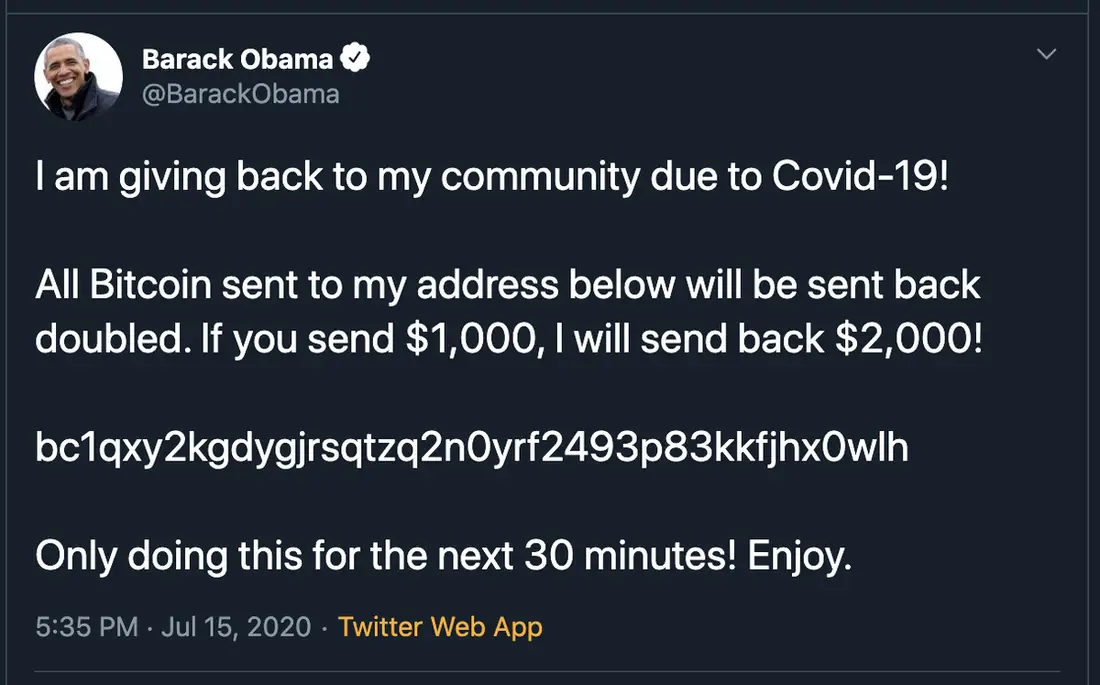
\includegraphics[width=\textwidth]{thanks-obama}
\end{frame}

%TODO OVERVIEW
%TODO2 questions for Alex
%TODO3 image formatting/sizing questions

\section{What Will You Learn Today?}

\begin{frame}{What Will You Learn Today?}
    \Large
    \begin{itemize}
        \item Digital Identity Relationships
        \item Basic and Advanced Authentication Flows
        \item Threats to Authentication
        \item Defense Against the Dark Arts
        \item Emerging Threats
    \end{itemize}
\end{frame}

\section{Digital Identity Mappings}

\begin{frame}{Digital Identity Mappings}
    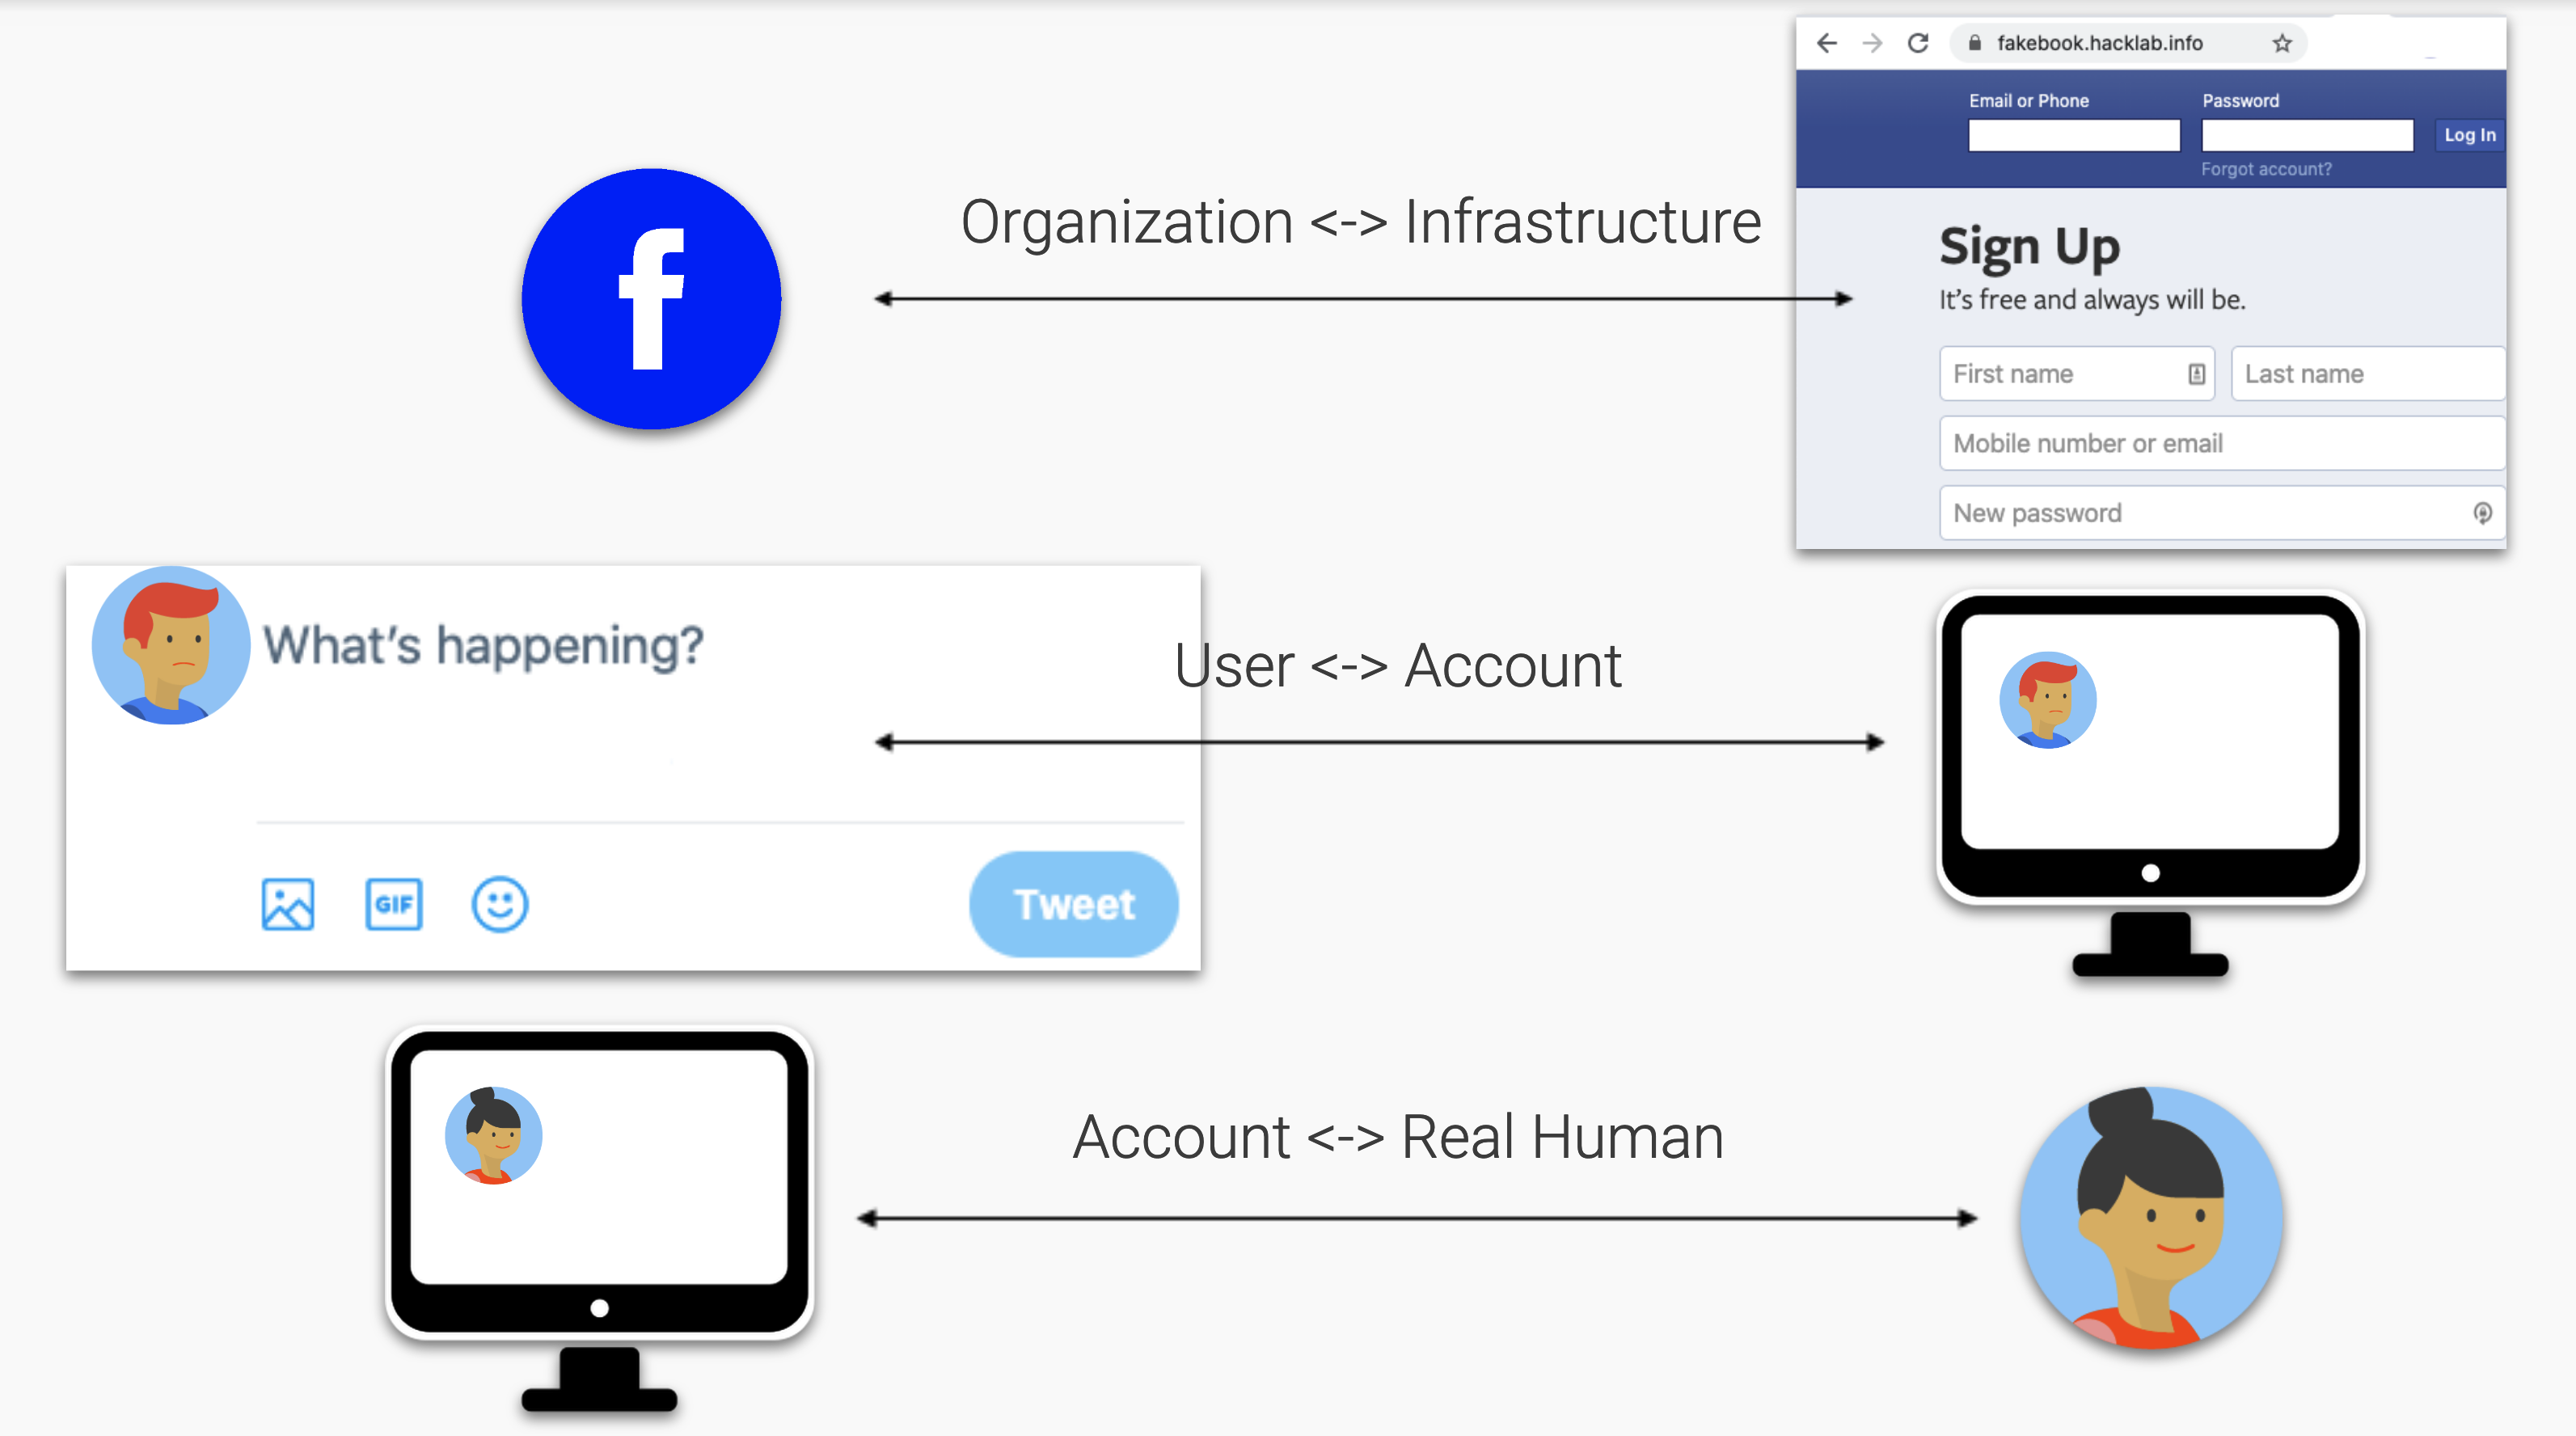
\includegraphics[width=\textwidth]{digital-identity-mappings}
\end{frame}

\begin{frame}{Account <-> Real Human}
    \begin{columns}
        \column{0.5\textwidth}
            \begin{itemize}
                \item Impersonating accounts
                \item Romance scams
                \item Advance fee fraud
                \item Physical good fraud
            \end{itemize}
            \vspace{0.05\textheight}
            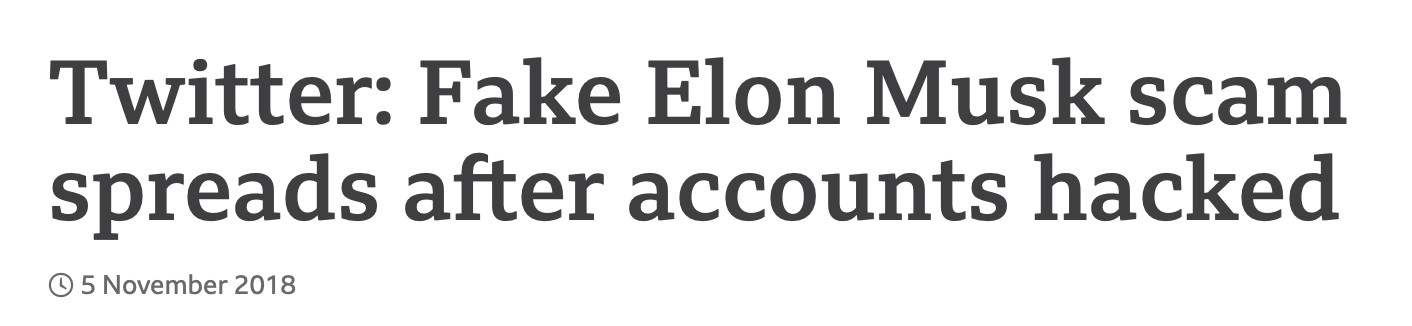
\includegraphics[width=\textwidth]{musk-scam-headline}
            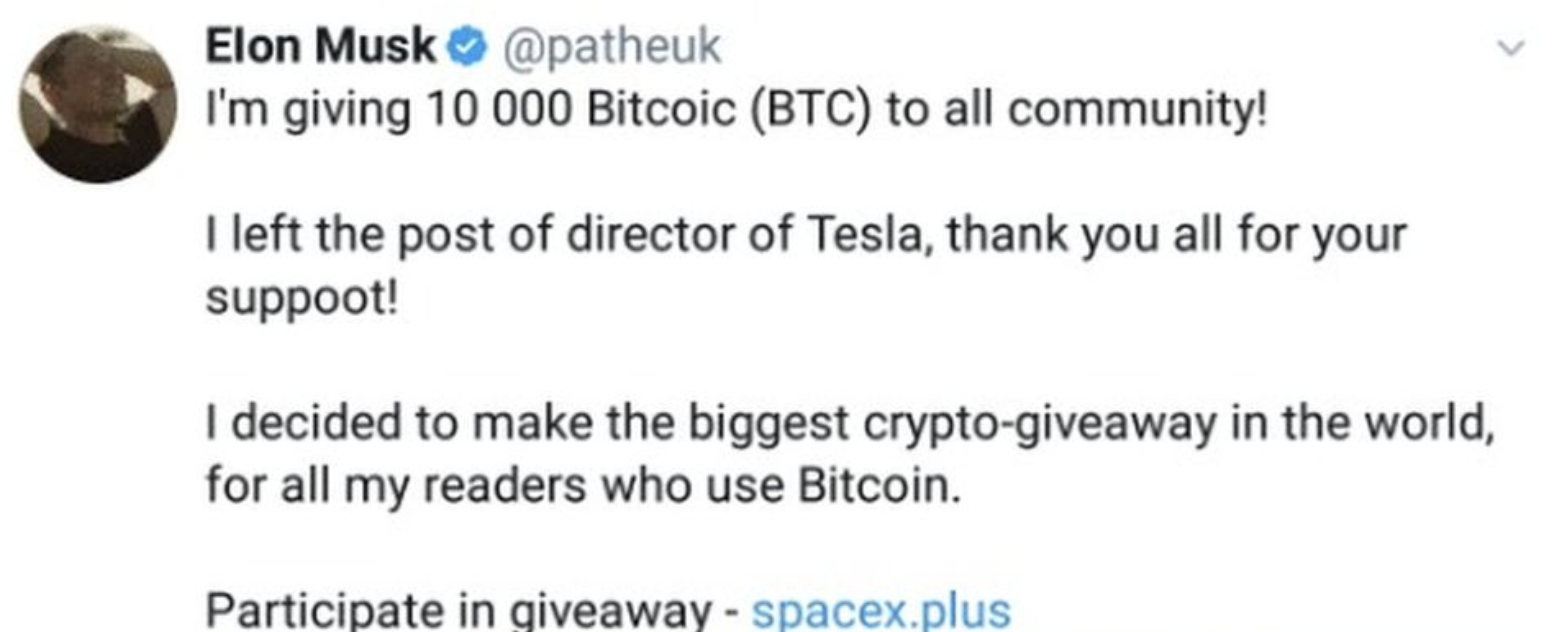
\includegraphics[width=\textwidth]{musk-scam-tweet}
        \column{0.5\textwidth}
            
\includegraphics[width=\textwidth]{fake-stamos-twitter}
    \end{columns}
\end{frame}

\begin{frame}{User <-> Account}
    \begin{columns}
        \column{0.6\textwidth}
            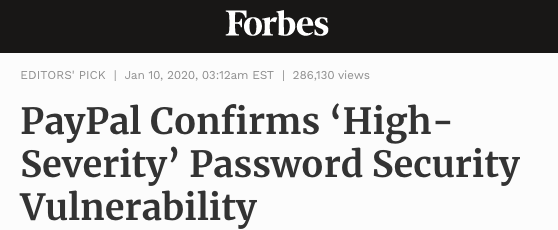
\includegraphics[width=\textwidth]{paypal-breach}
            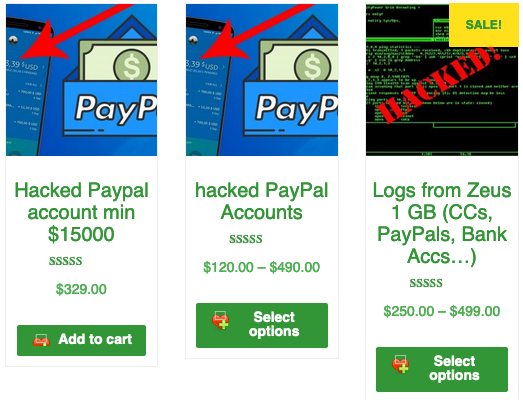
\includegraphics[width=\textwidth]{hacked-paypal-accounts}
        \column{0.4\textwidth}
            \begin{itemize}
                \item Stealing passwords
                \item Cracked breached password databases
                \item Credential stuffing
                \item Malware (Trojans)
            \end{itemize}
    \end{columns}
\end{frame}

\begin{frame}{Organization <-> Infrastructure }
    \begin{columns}
        \column{0.45\textwidth}
            \begin{itemize}
                \item Phishing 
                \item Meddler-In-The Middle (MITM) attacks
                \item Typosquatting
                \item Mismatched domains
                \item Internationalized Domain Name (IDN) Homograph attack
                \item Email security
            \end{itemize}
        \column{0.55\textwidth}
            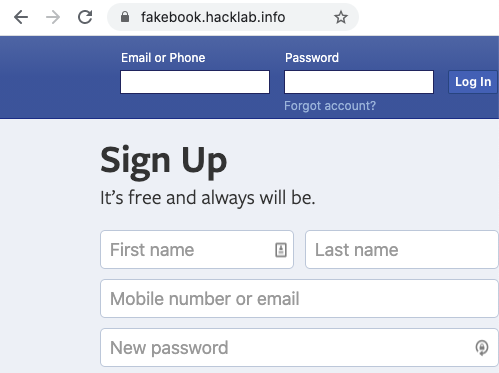
\includegraphics[width=\textwidth]{fakebook-login}
    \end{columns}
\end{frame}

\begin{frame}{Black Markets Allow For Specialization of Effort}
    \begin{columns}
        \column{0.5\textwidth}
            There are:
            \begin{itemize}
                \item Markets for stolen data
                \item Easy-to-use malware, like keyloggers 
                \item Phishing kits
                \item Hackers for hire
                \item Botnets 
            \end{itemize}
            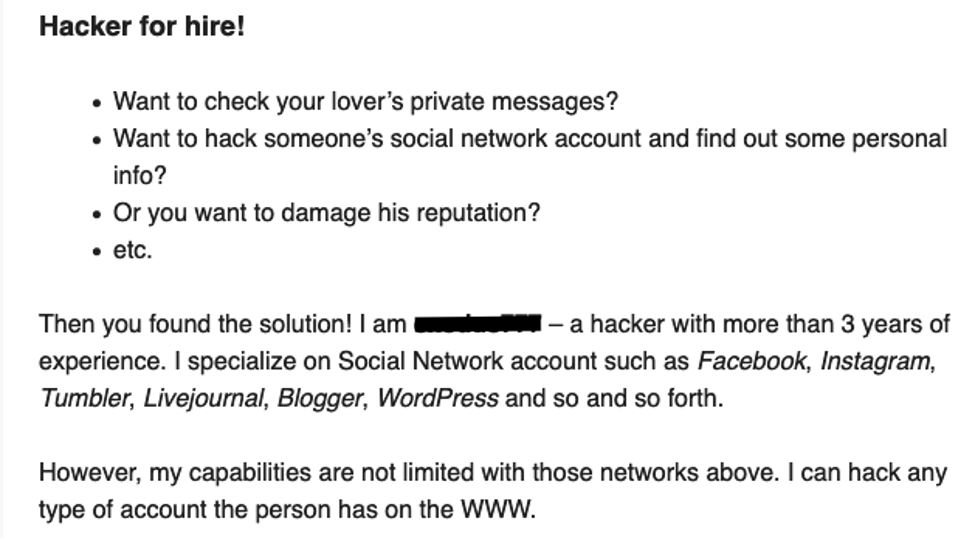
\includegraphics[width=\textwidth]{hacker-for-hire}
        \column{0.5\textwidth}
            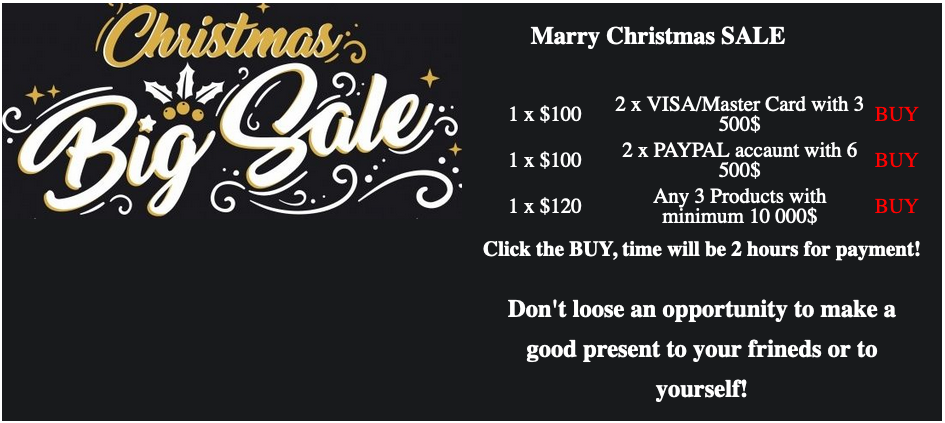
\includegraphics[width=\textwidth]{marry-christmas-sale}
    \end{columns}
\end{frame}

\begin{frame}{Why Should I Care?}
    There are multiple levels of identity online and strong authentication is essential for them all.\\~\\
    Protecting users while maintaining availability requires a complex web of systems covering Prevention, Detection, and Mitigation.
\end{frame}

\section{Authentication}

\begin{frame}{Authn vs Authz}
    \large
    \textbf{Authentication (authn)} - Whether users are who they claim to be\\~\\
    \textbf{Authorization (authz)} - What users are and aren’t allowed to access
\end{frame}

\begin{frame}{How Does Authentication Work?}
    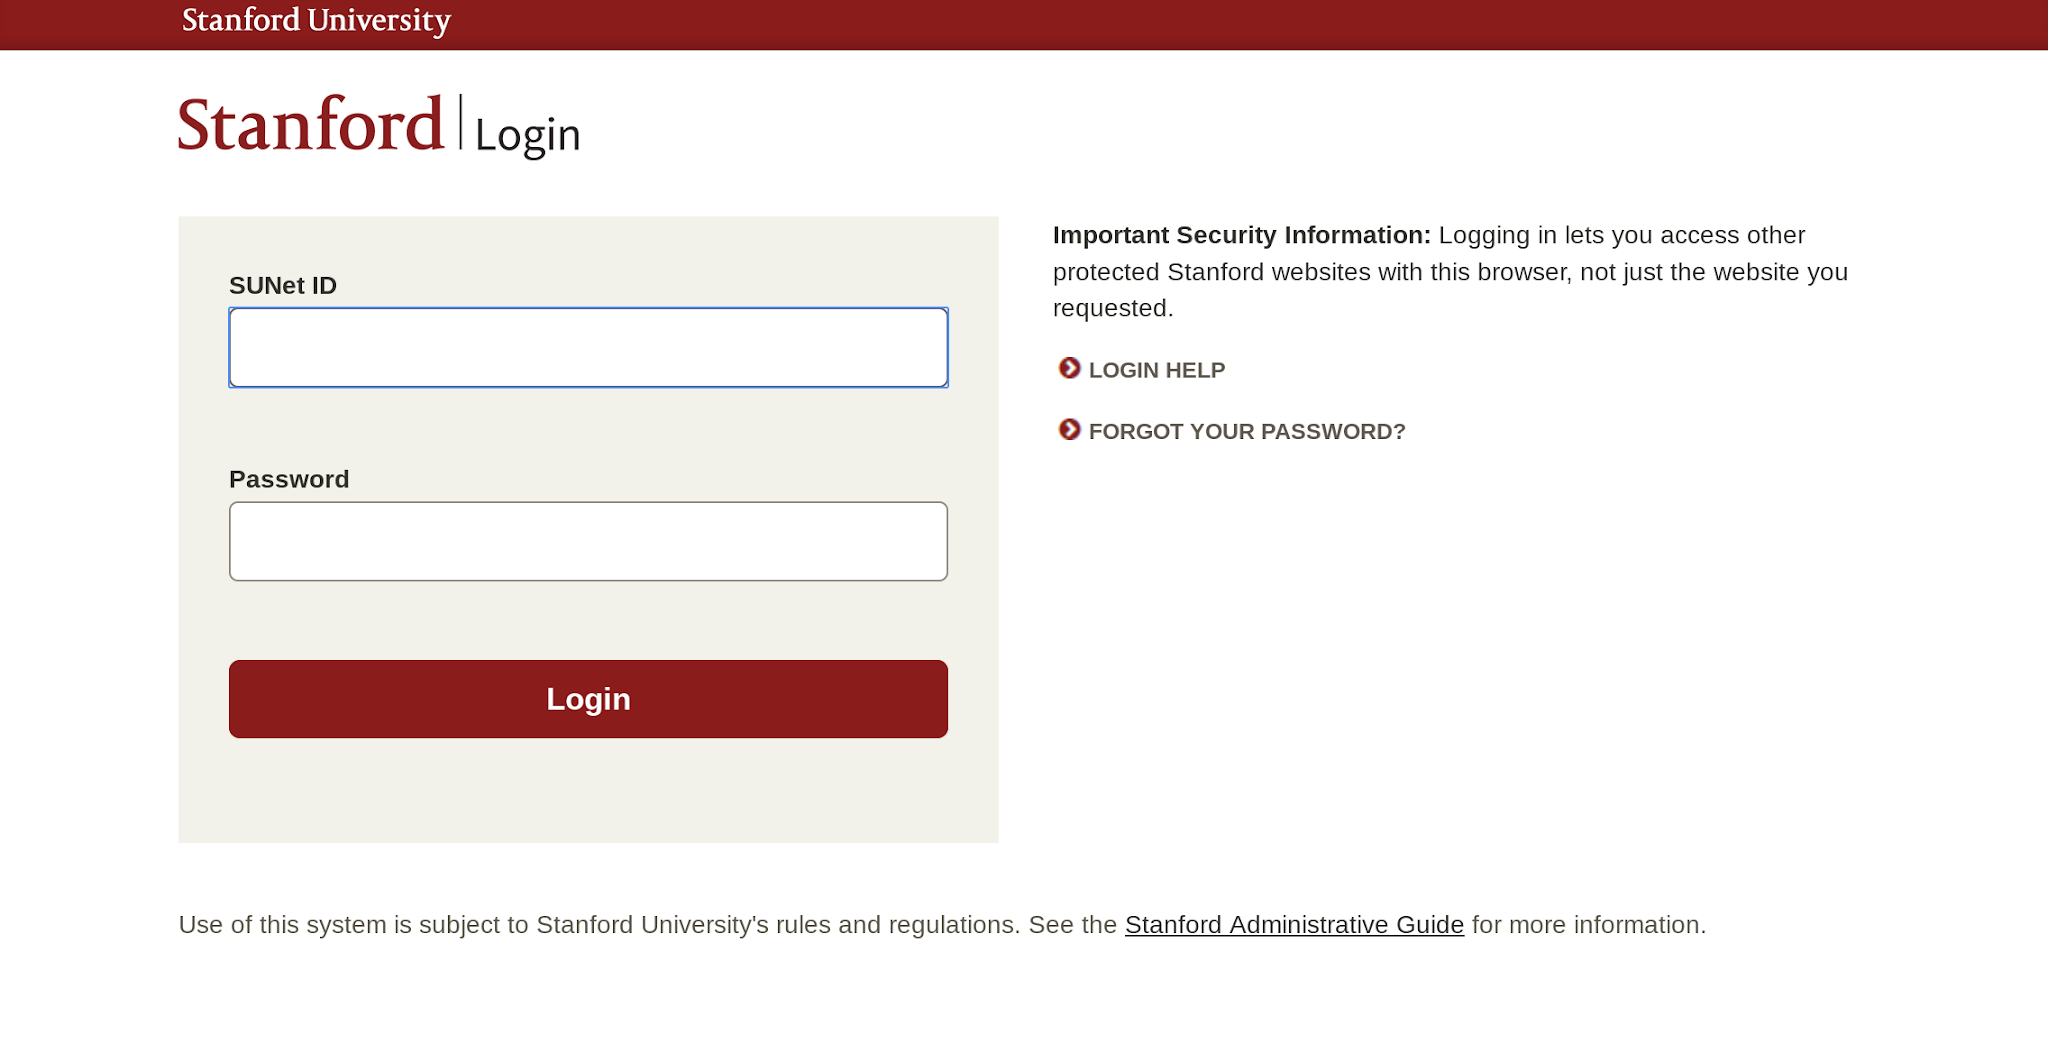
\includegraphics[width=\textwidth]{stanford-login}
\end{frame}

\begin{frame}{How Does Authentication Work?}
    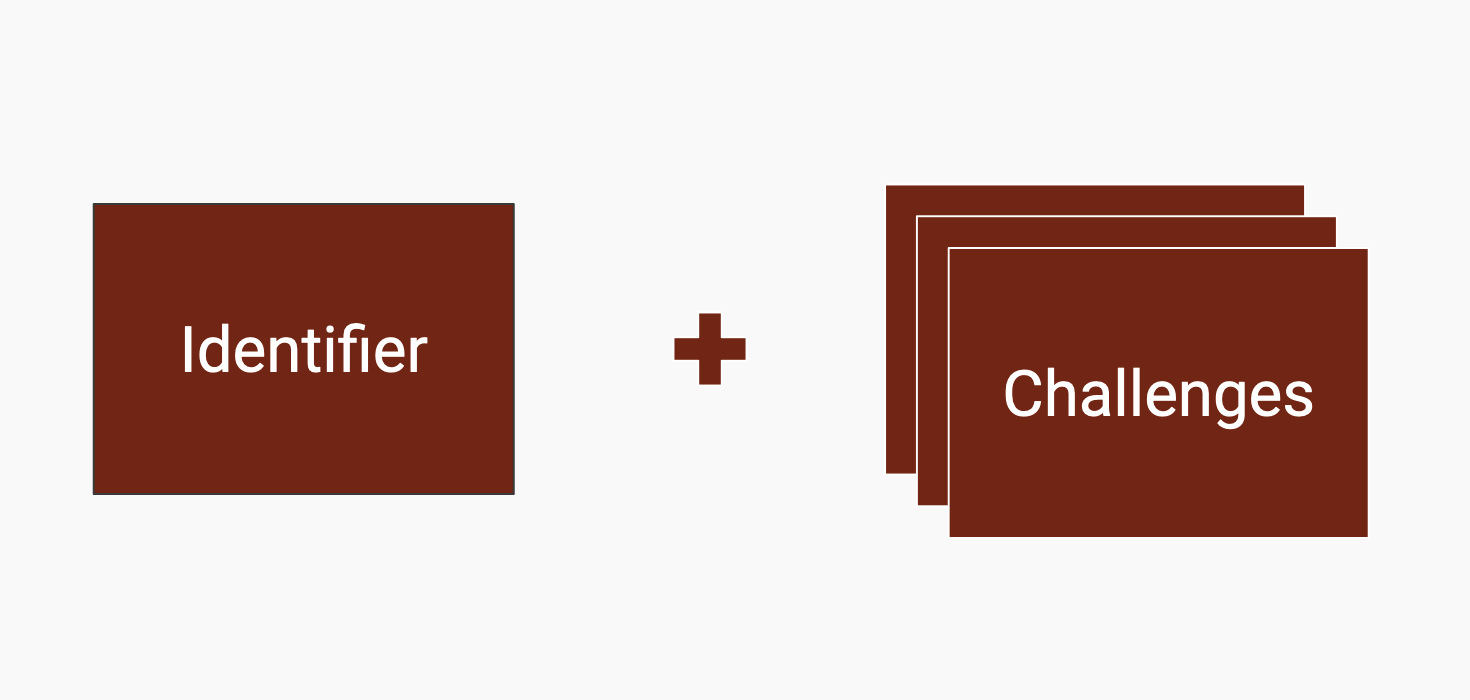
\includegraphics[width=\textwidth]{auth}
\end{frame}

\begin{frame}{}%TODO3 alignment
    \thispagestyle{empty}
    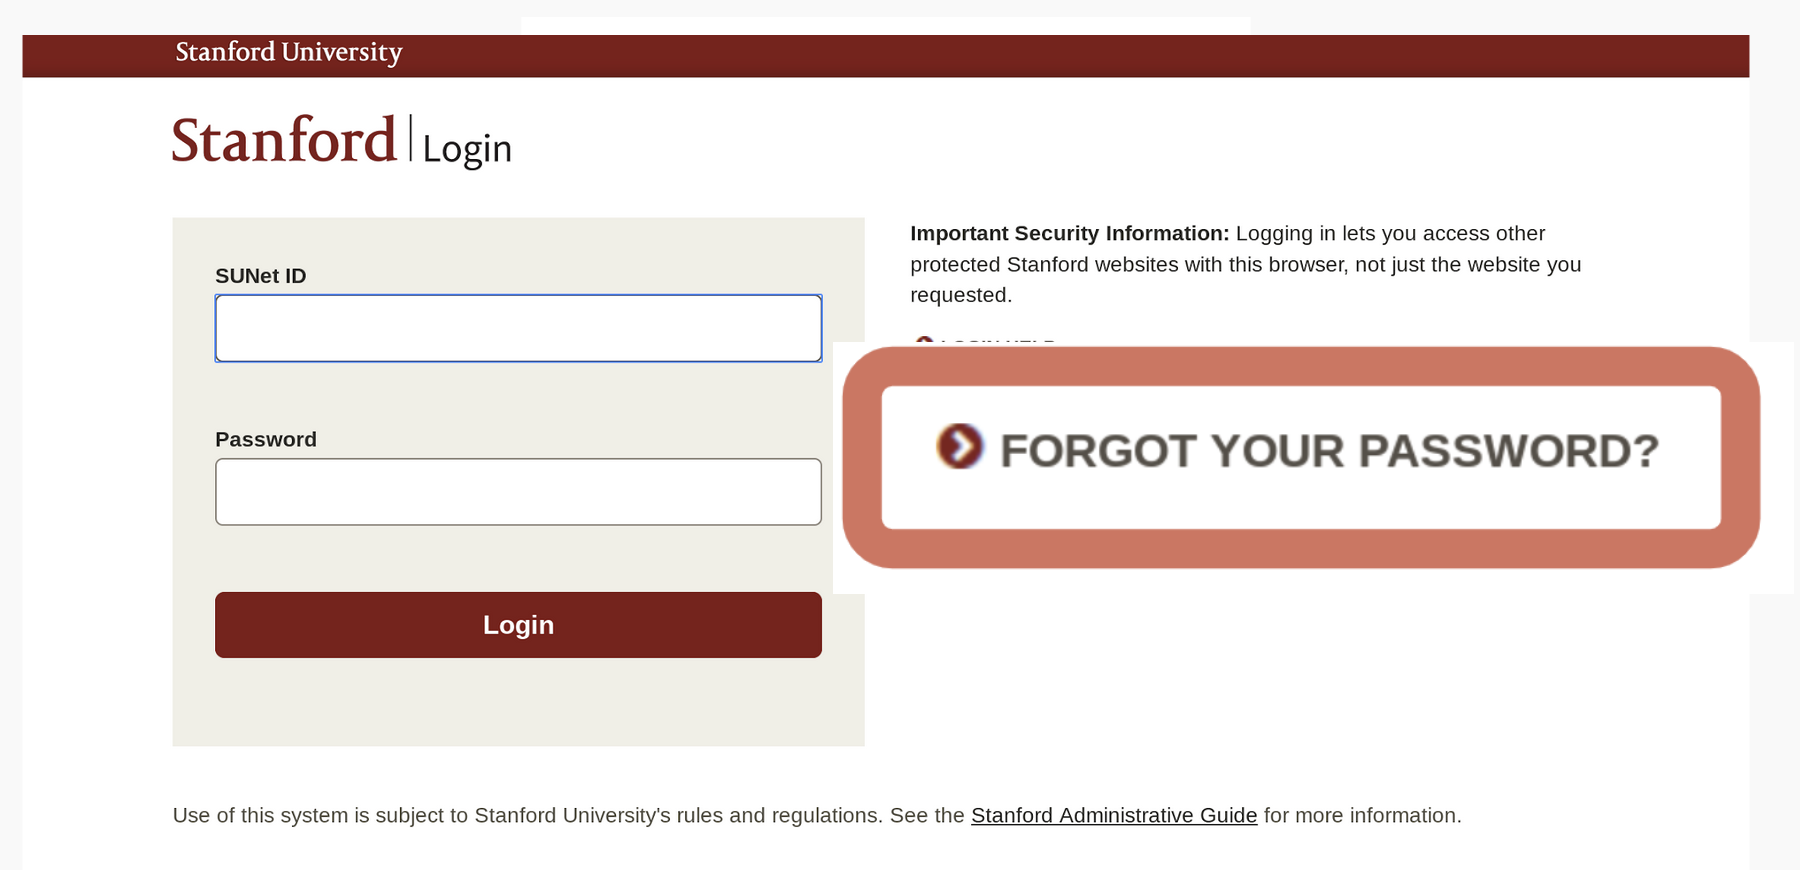
\includegraphics[width=\paperwidth]{stanford-forgot-password}
\end{frame}

\begin{frame}{}%TODO3 alignment
    \thispagestyle{empty}
    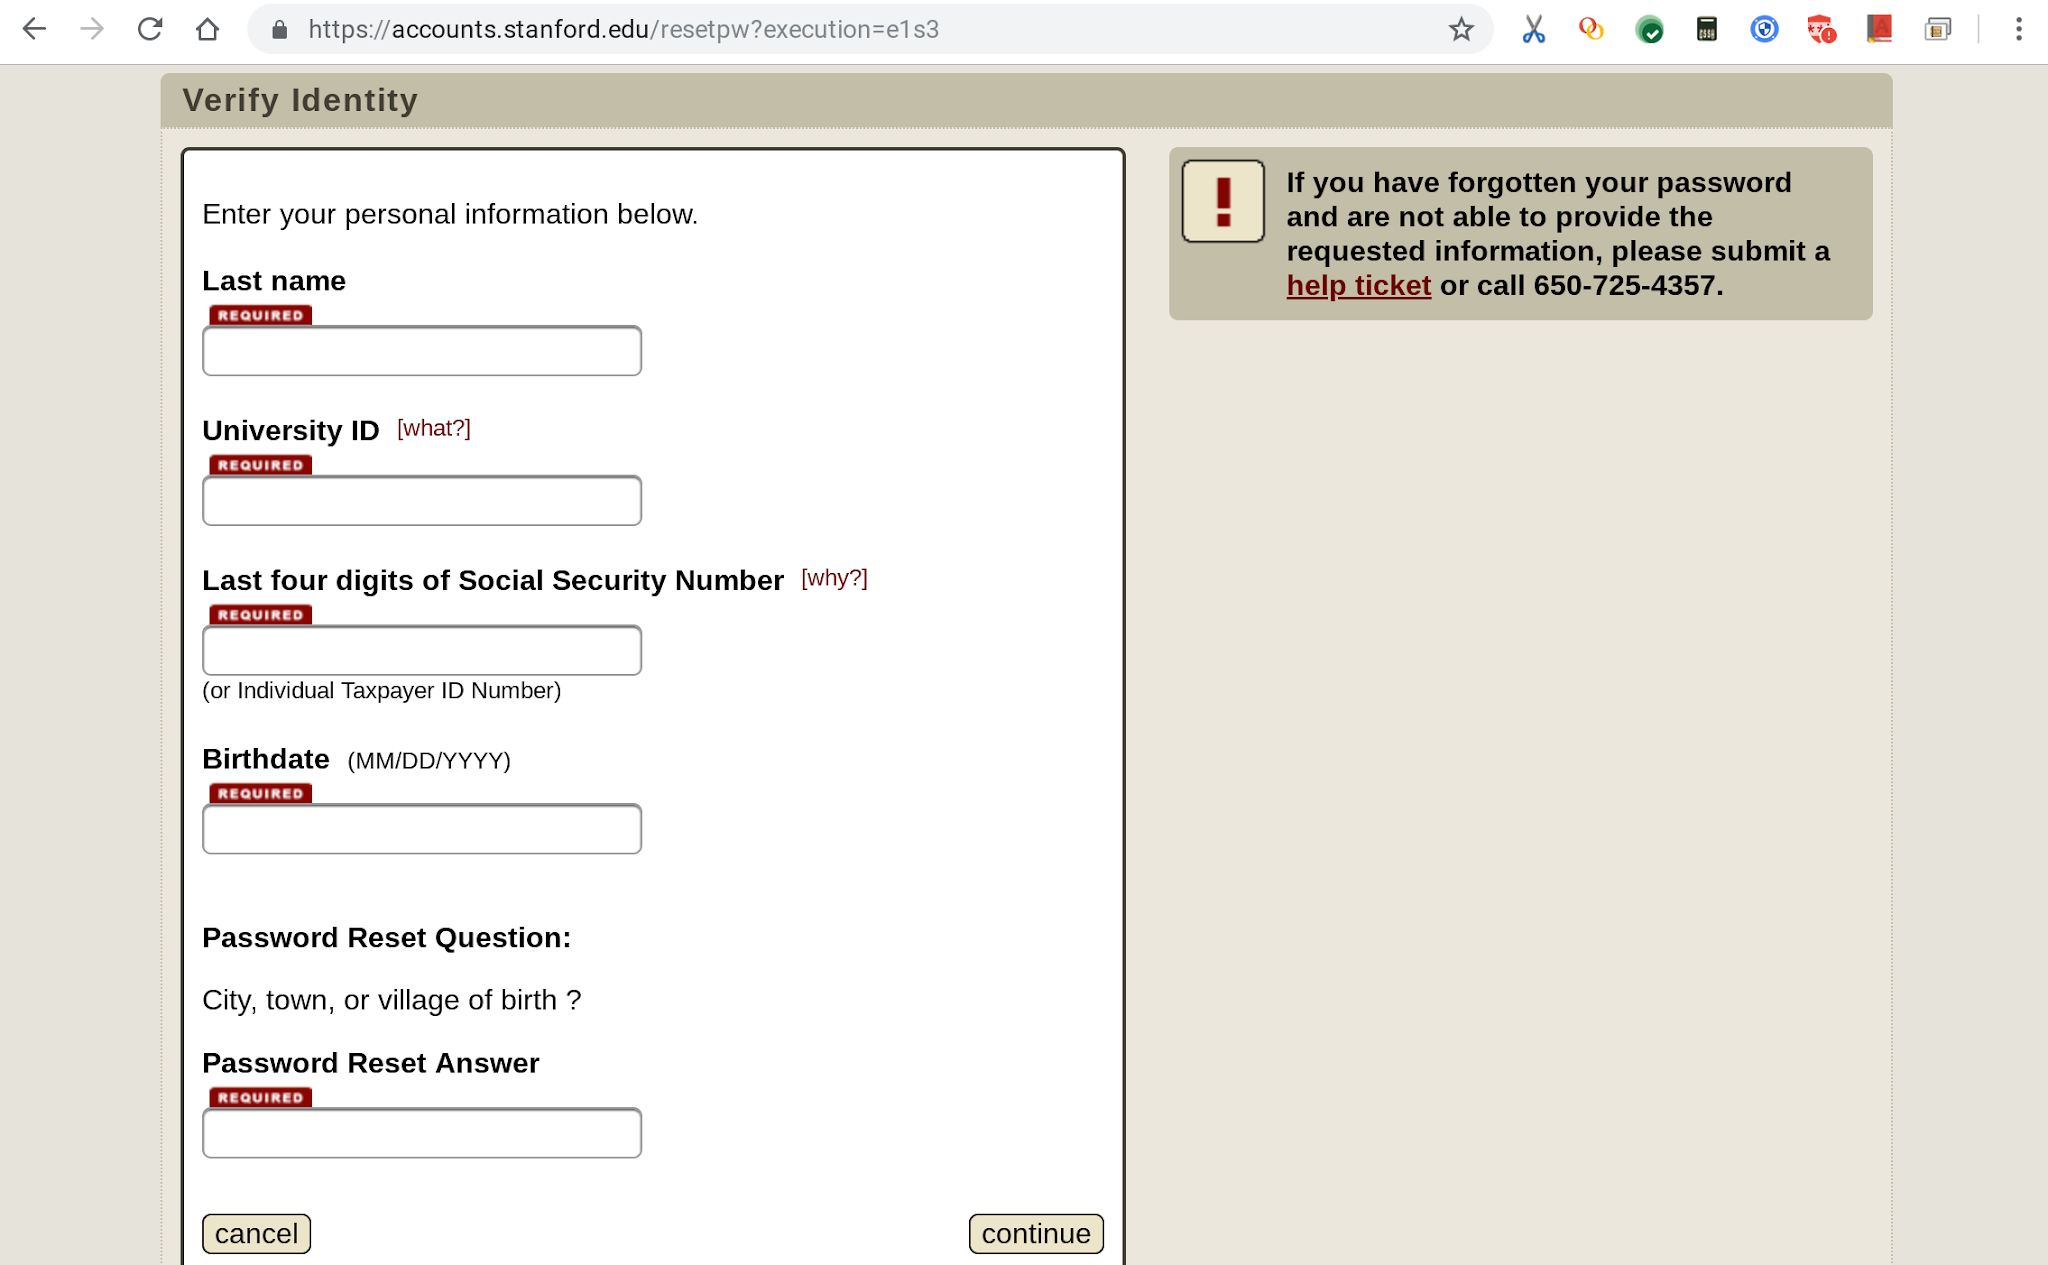
\includegraphics[width=\paperwidth]{stanford-id-verification}
\end{frame}

\begin{frame}{Multi-factor}
    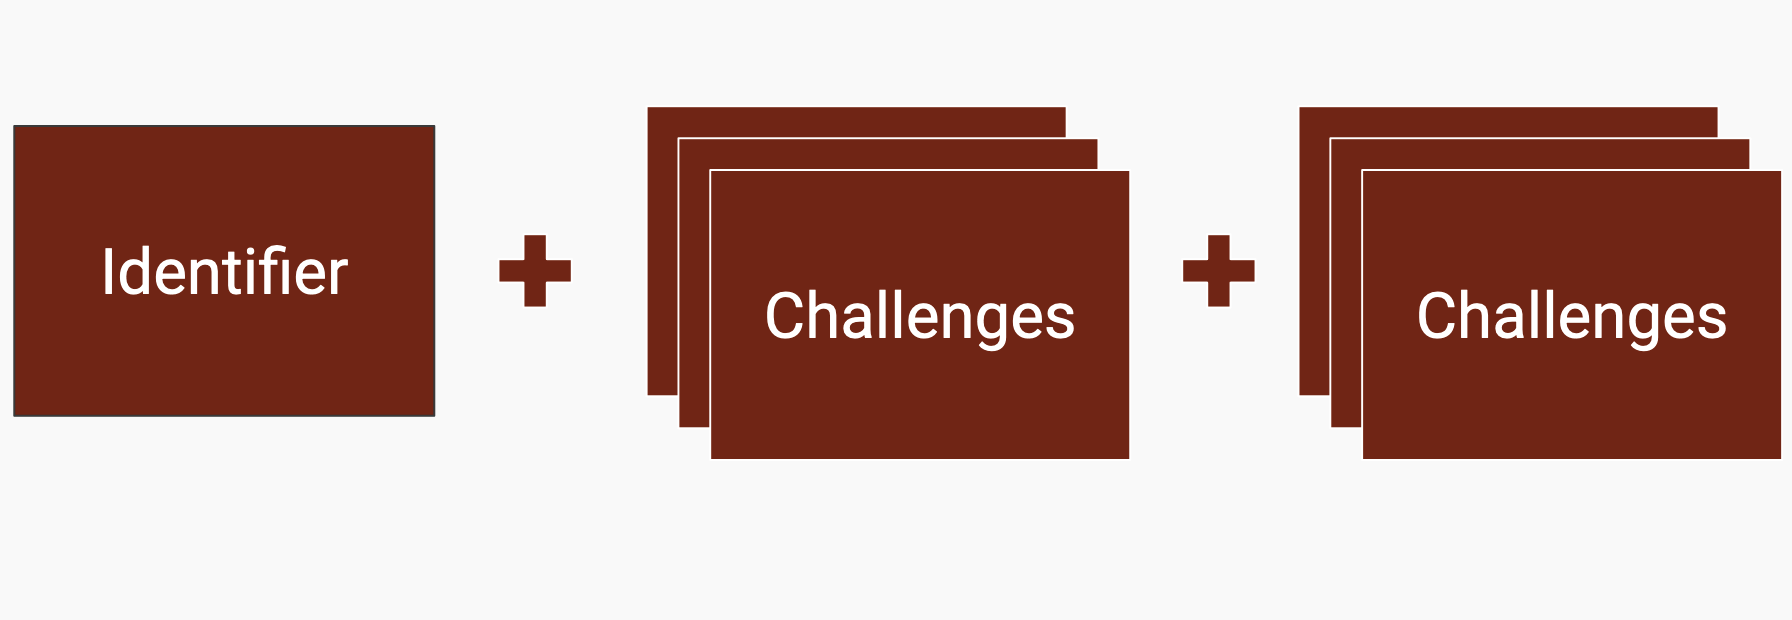
\includegraphics[width=\textwidth]{multifactor-auth}
\end{frame}

\begin{frame}{}%TODO3 alignment
    \centering
    \thispagestyle{empty}
    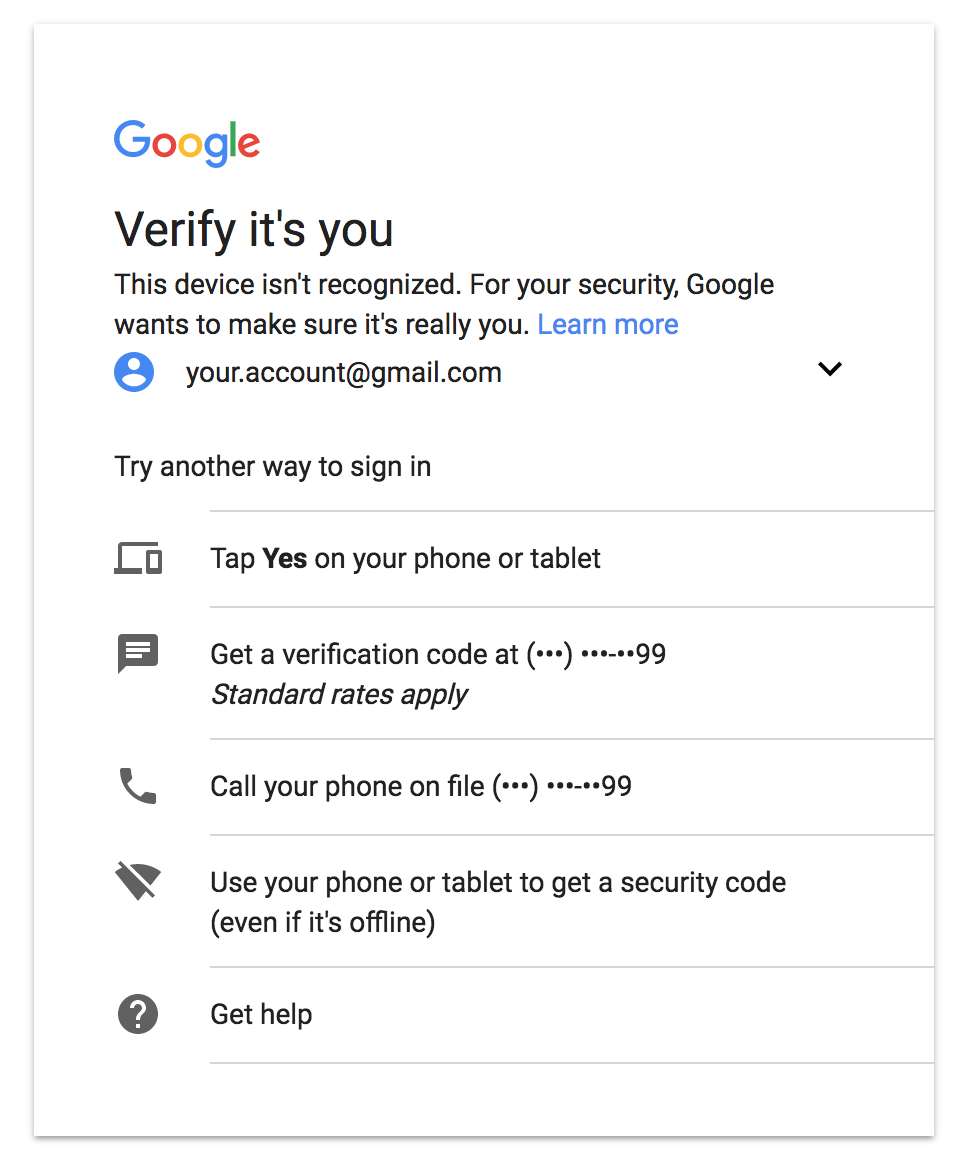
\includegraphics[height=\textheight]{google-2fa}
\end{frame}

\begin{frame}{Adoption of Security Measures}
    \begin{columns}
        \column{0.7\textwidth}
            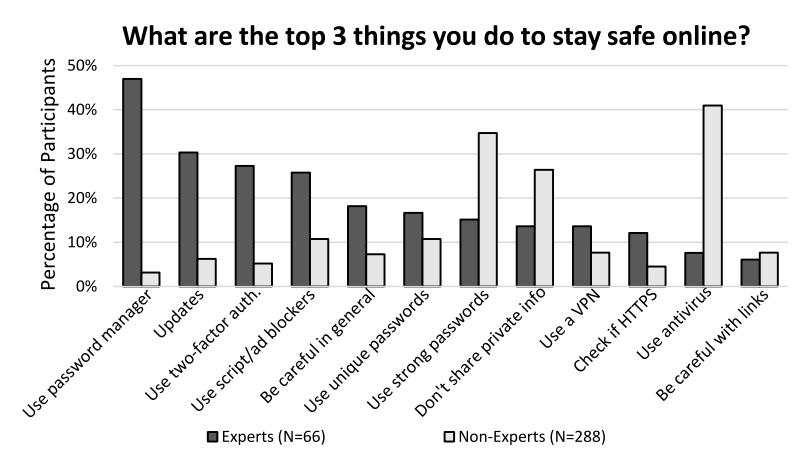
\includegraphics[width=\textwidth]{stay-safe-online}
            \tiny
            Source:\\
            Replication: No One Can Hack My Mind (Busse  et al.)\\
            \url{https://www.usenix.org/system/files/soups2019-busse.pdf}
        \column{0.3\textwidth}
            <10\% 2FA of active Google accounts\\~\\
            ~22.5\% of Americans use a password manager app (YouGov Survey 2020)
    \end{columns}
\end{frame}

\section{Threats}

\begin{frame}{Threats}
    \Large
    \begin{itemize}
        \item Credential breach
        \item Malware
        \item Phishing
        \item Active MITM
    \end{itemize}
\end{frame}

\begin{frame}{Quota Inversion}
    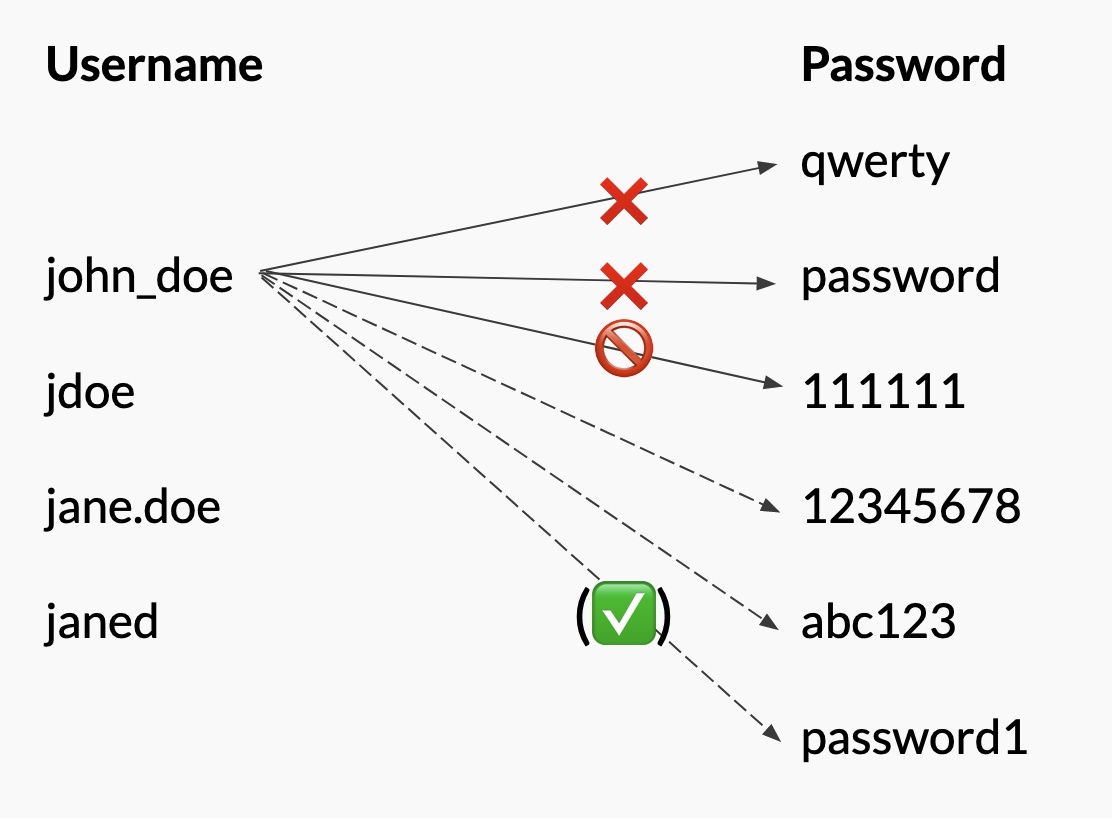
\includegraphics[width=\textwidth]{quota-inversion-1}
\end{frame}

\begin{frame}{Quota Inversion}
    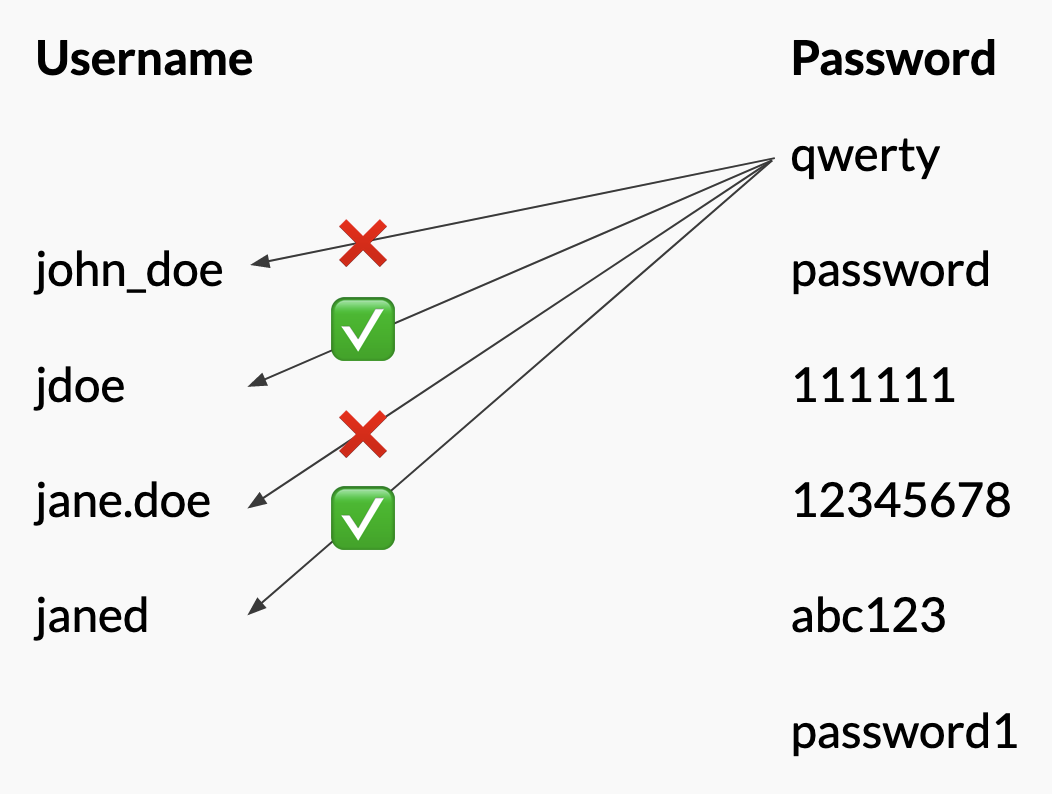
\includegraphics[width=\textwidth]{quota-inversion-2}
\end{frame}

\begin{frame}{}%TODO3 clear format?; sizing?
    \centering
    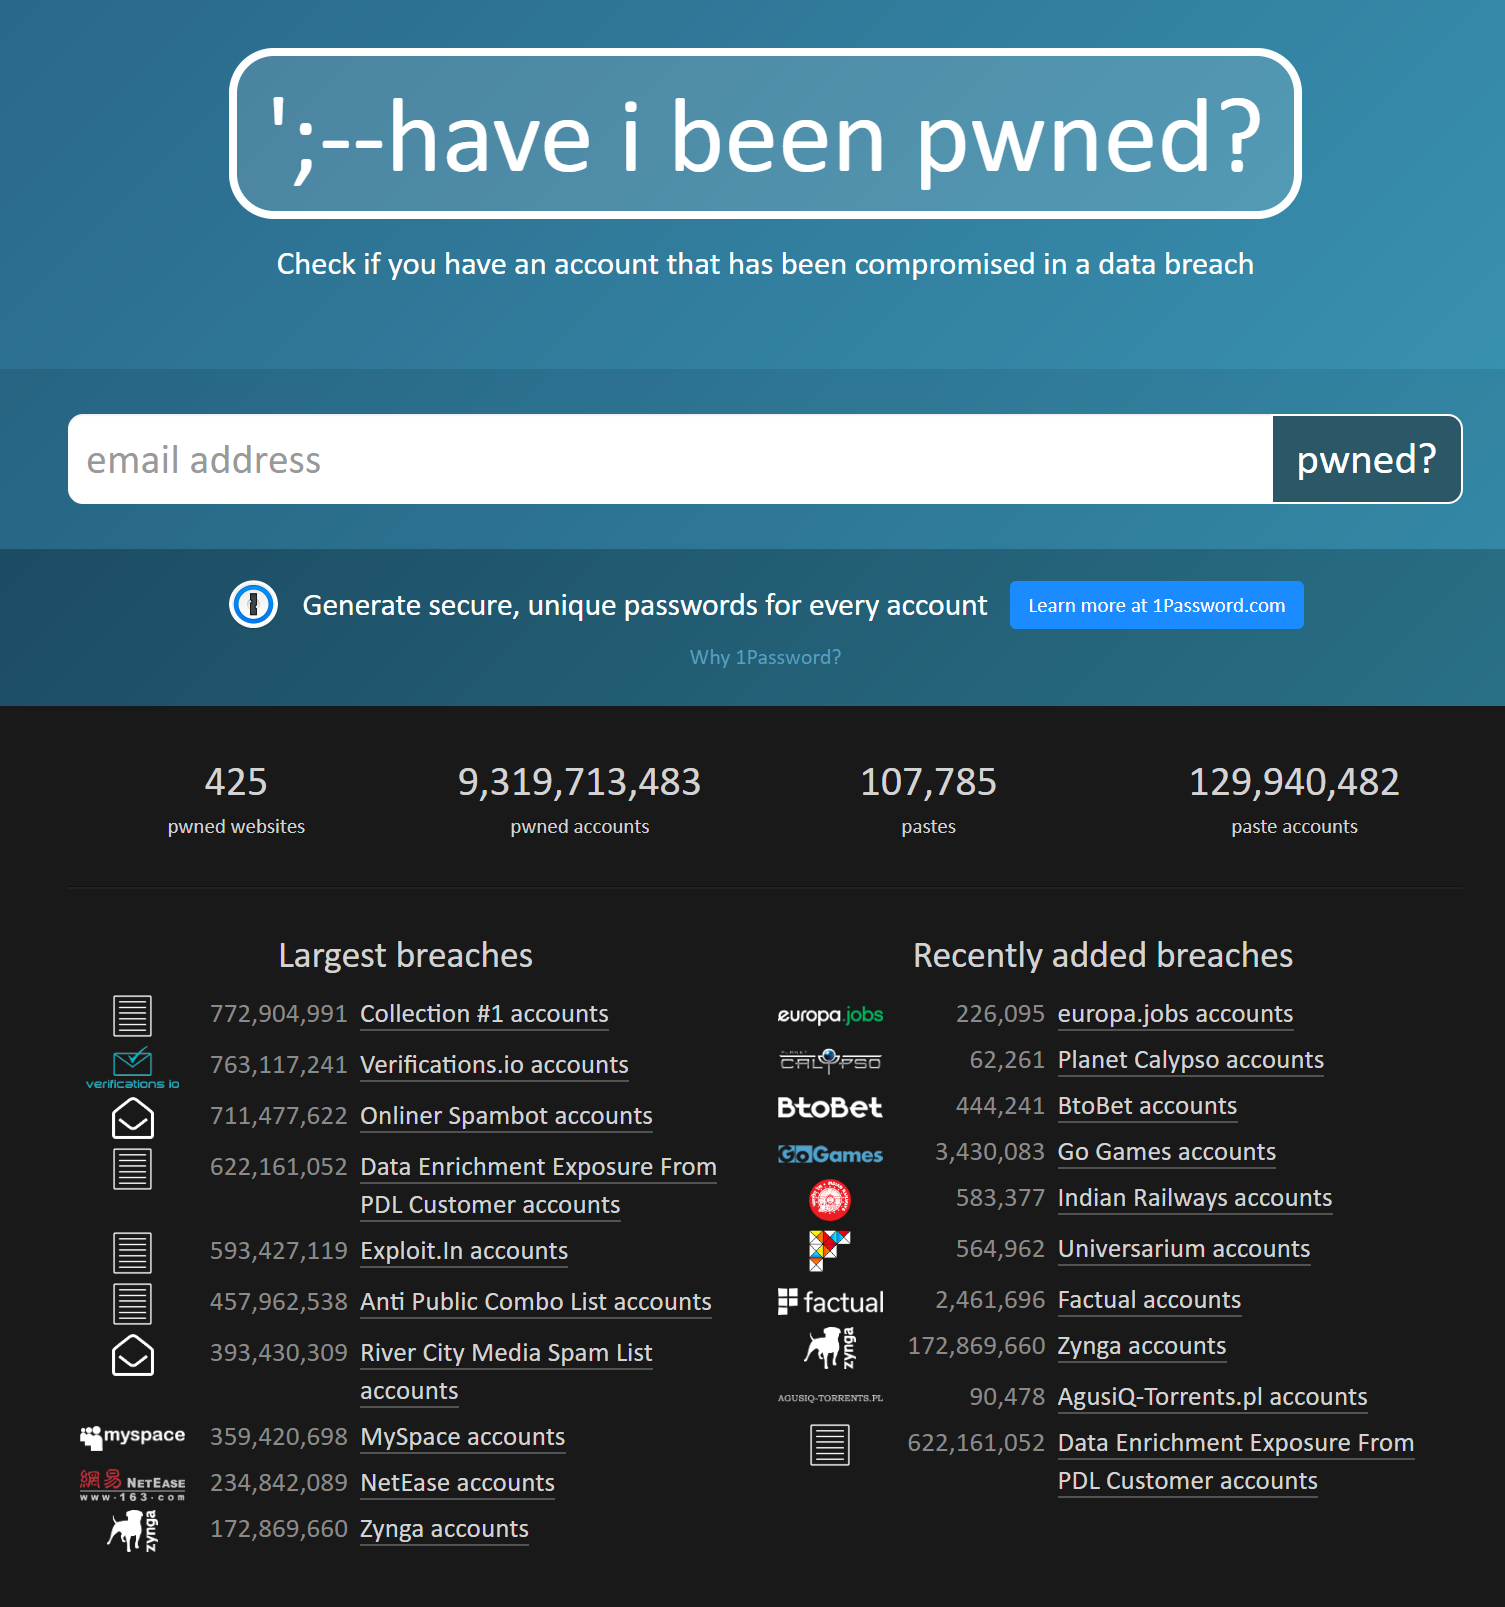
\includegraphics[height=\paperheight]{have-i-been-pwned}
\end{frame}

\begin{frame}{}
    \thispagestyle{empty}
    \AddToShipoutPictureBG*{\adjincludegraphics[trim=0 {0.36\height} 0 0, clip, width=\paperwidth]{predator13}}
\end{frame}

\begin{frame}{}
    \thispagestyle{empty}
    \begin{columns}
        \column{0.45\textwidth}
            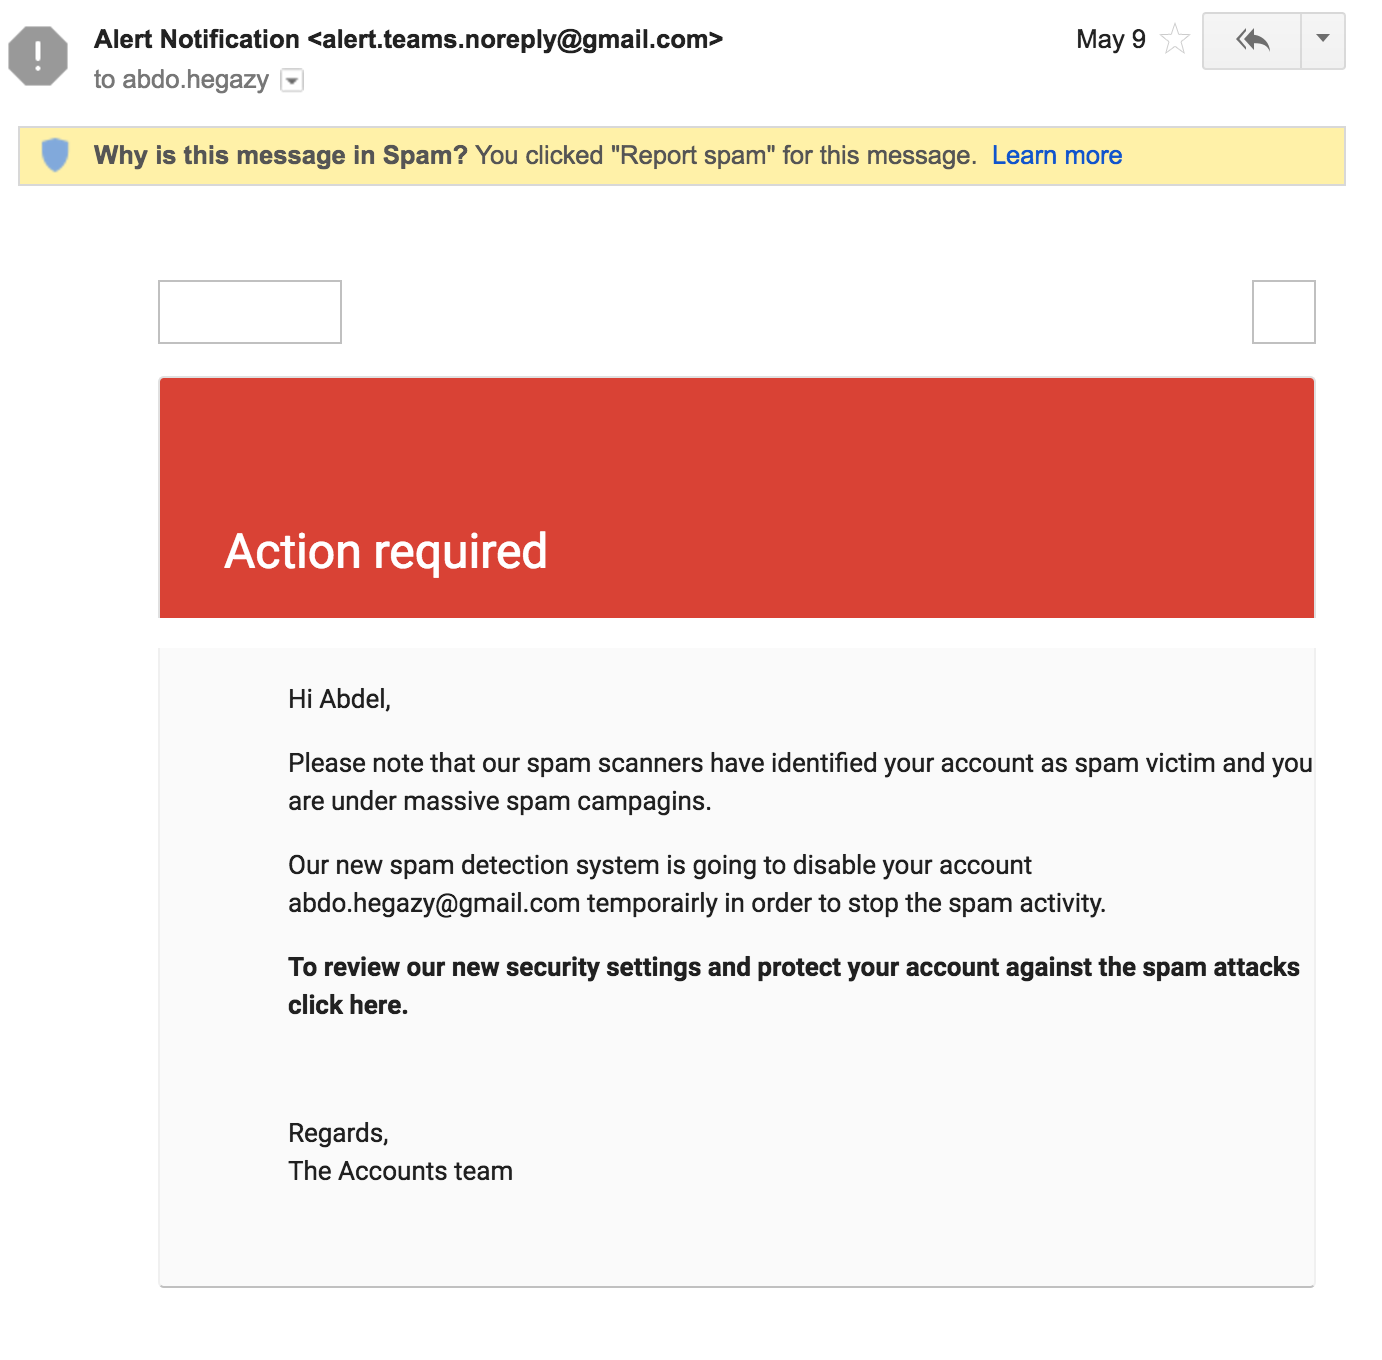
\includegraphics[width=\textwidth]{susmail1}
            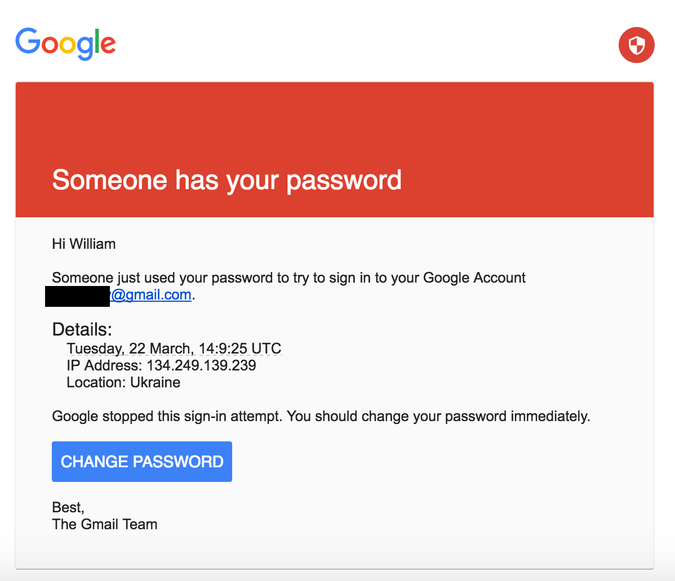
\includegraphics[width=\textwidth]{susmail3}
        \column{0.45\textwidth}
            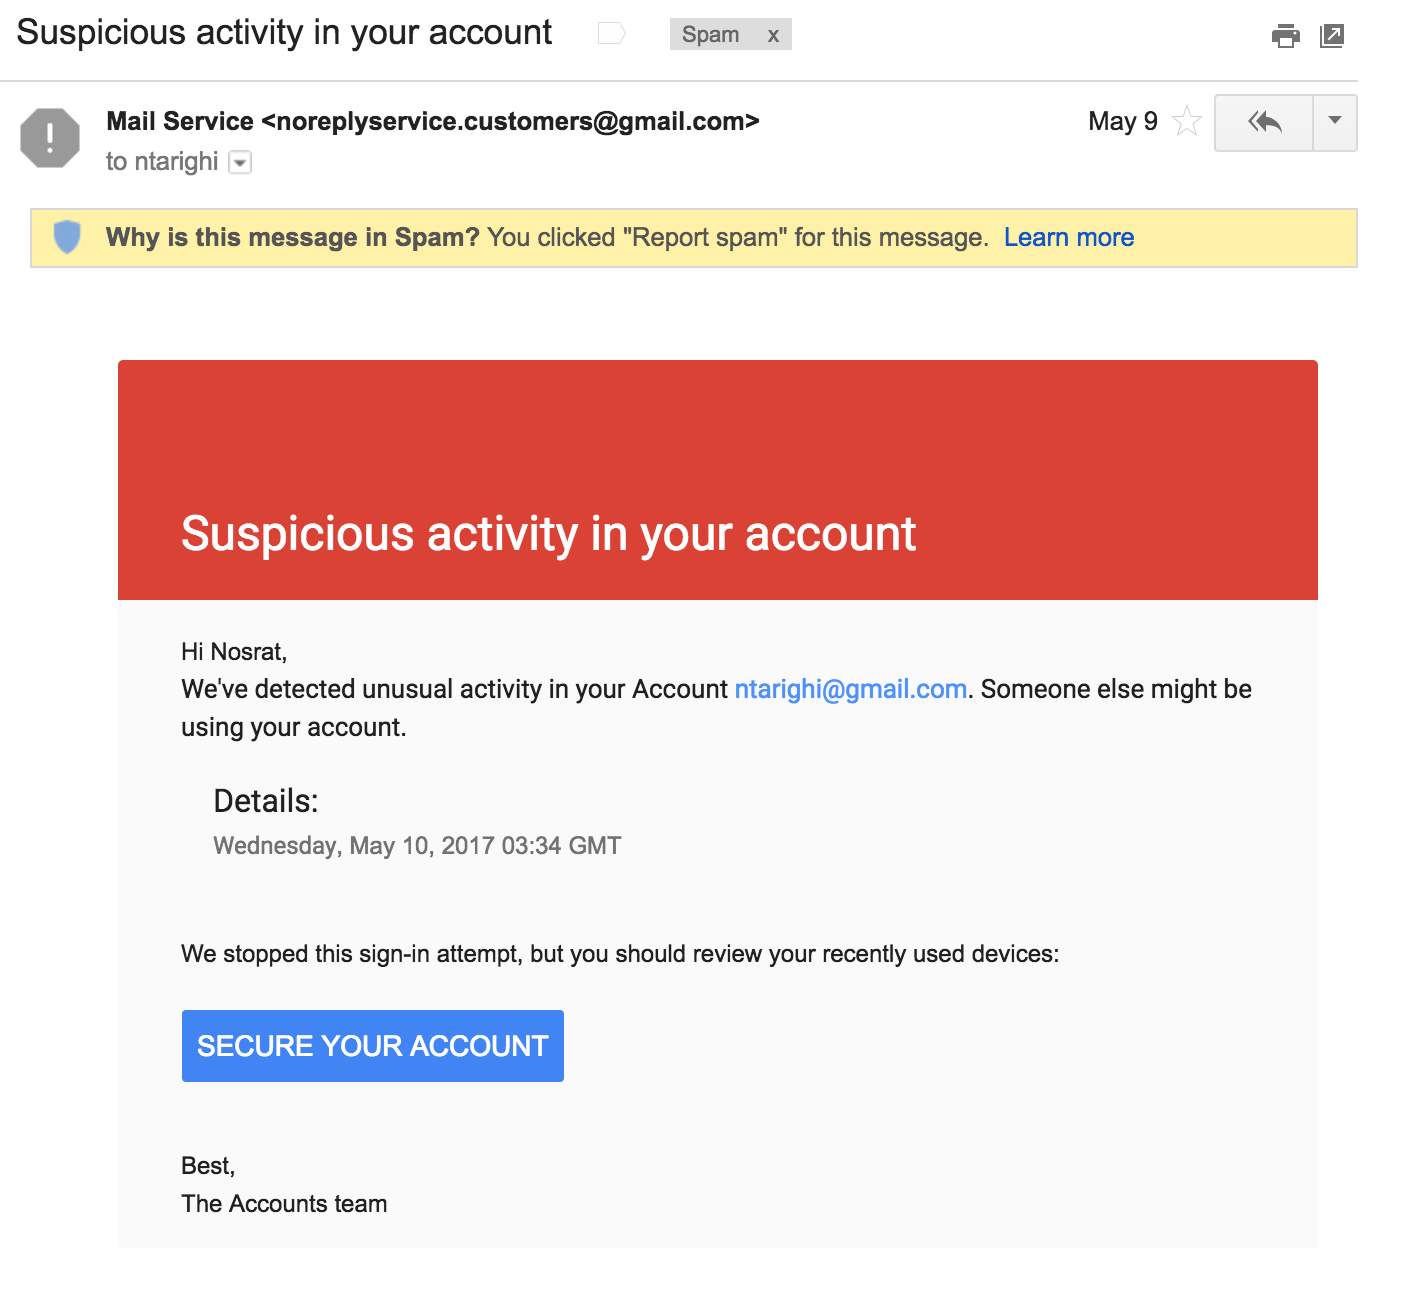
\includegraphics[width=\textwidth]{susmail2}
            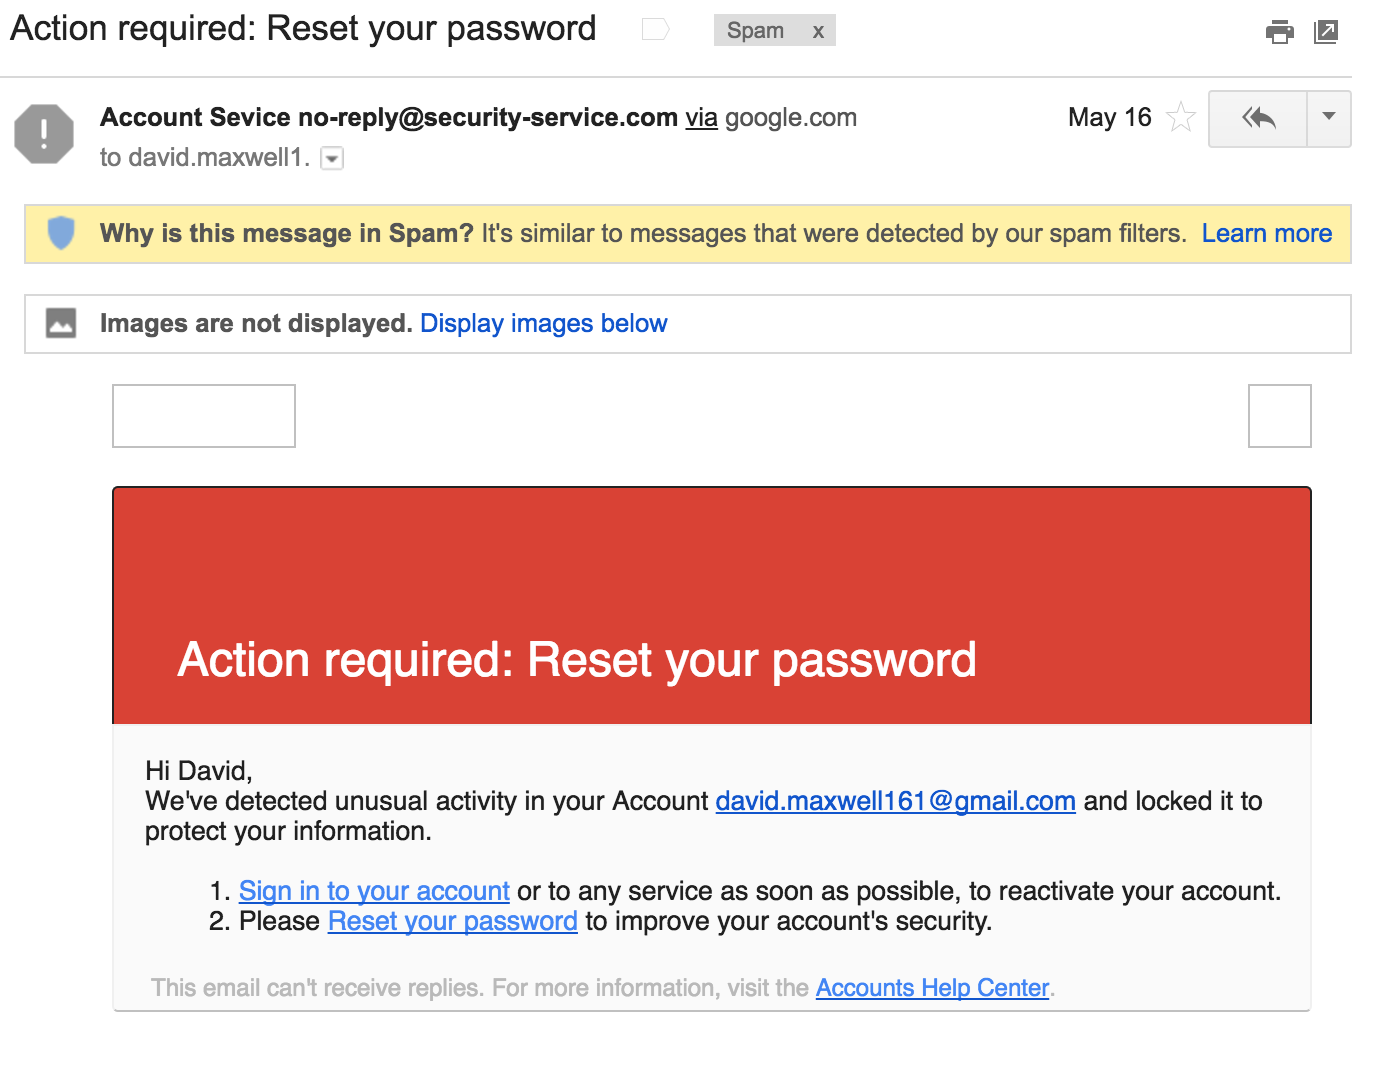
\includegraphics[width=\textwidth]{susmail4}
    \end{columns}
\end{frame}

\begin{frame}{}%TODO3
    \thispagestyle{empty}
    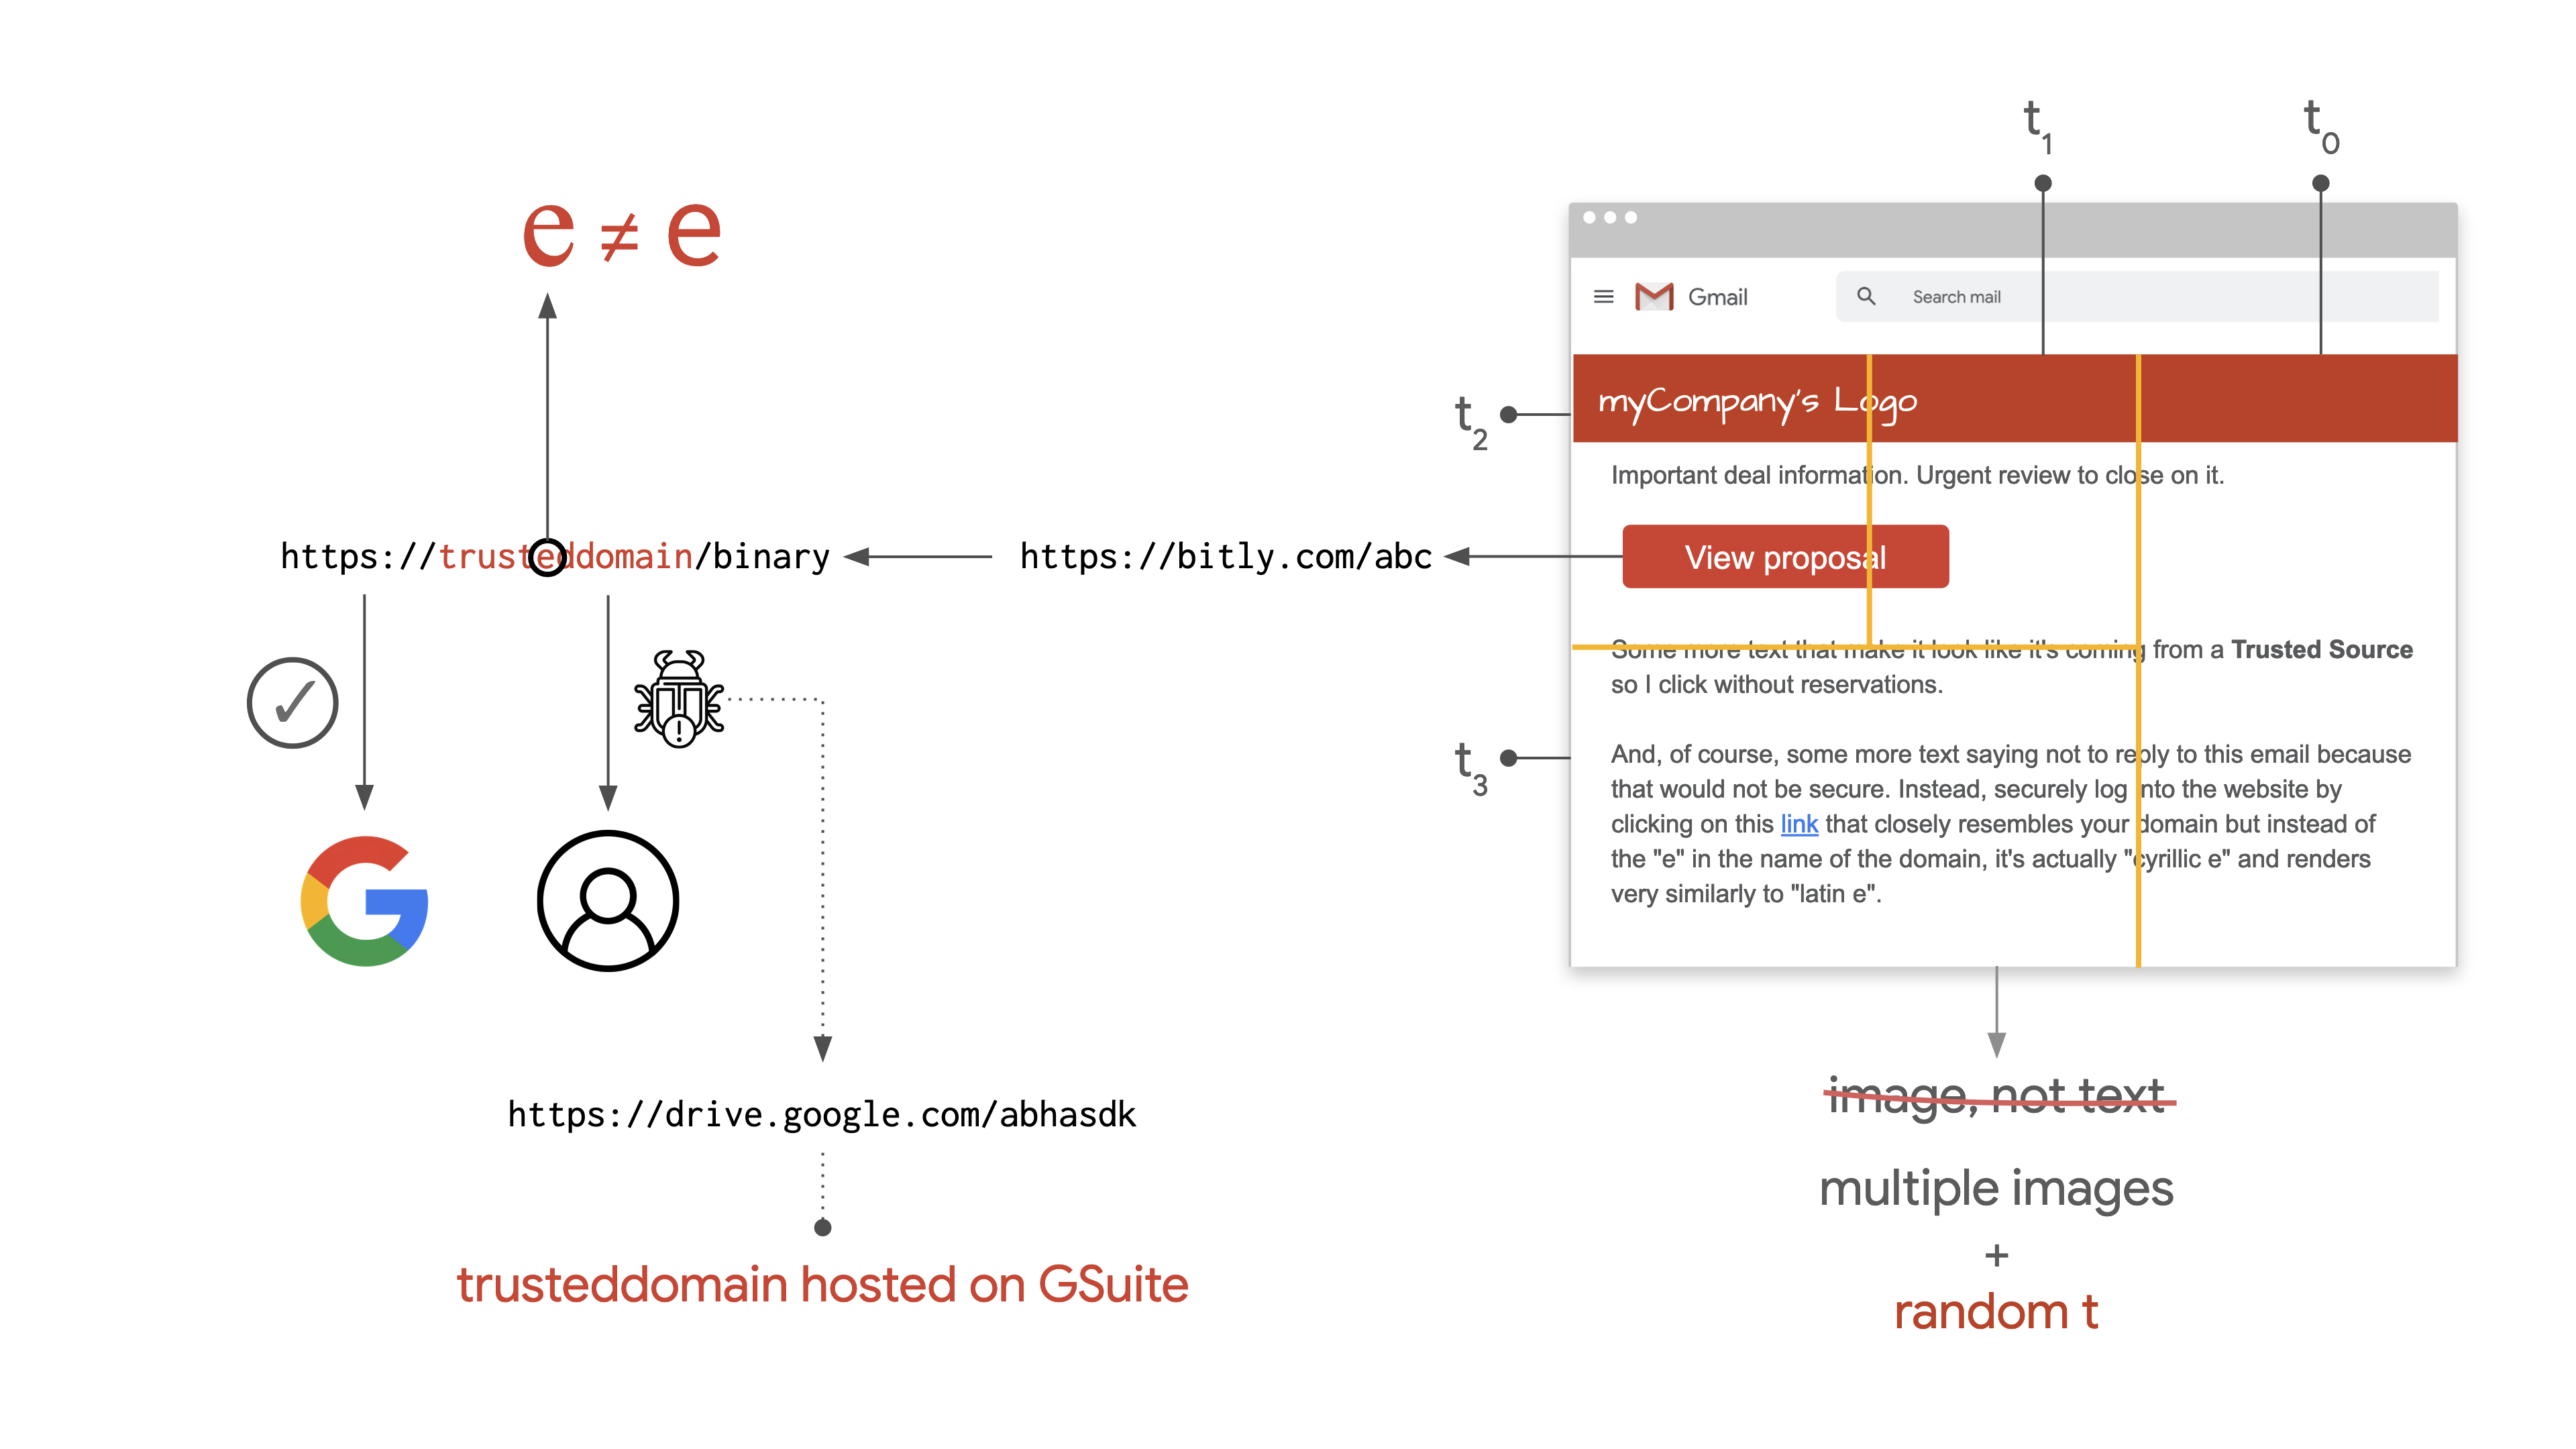
\includegraphics[width=\paperwidth]{anatomy-of-phishing-mail}
\end{frame}

\begin{frame}{}%TODO3
    \thispagestyle{empty}
    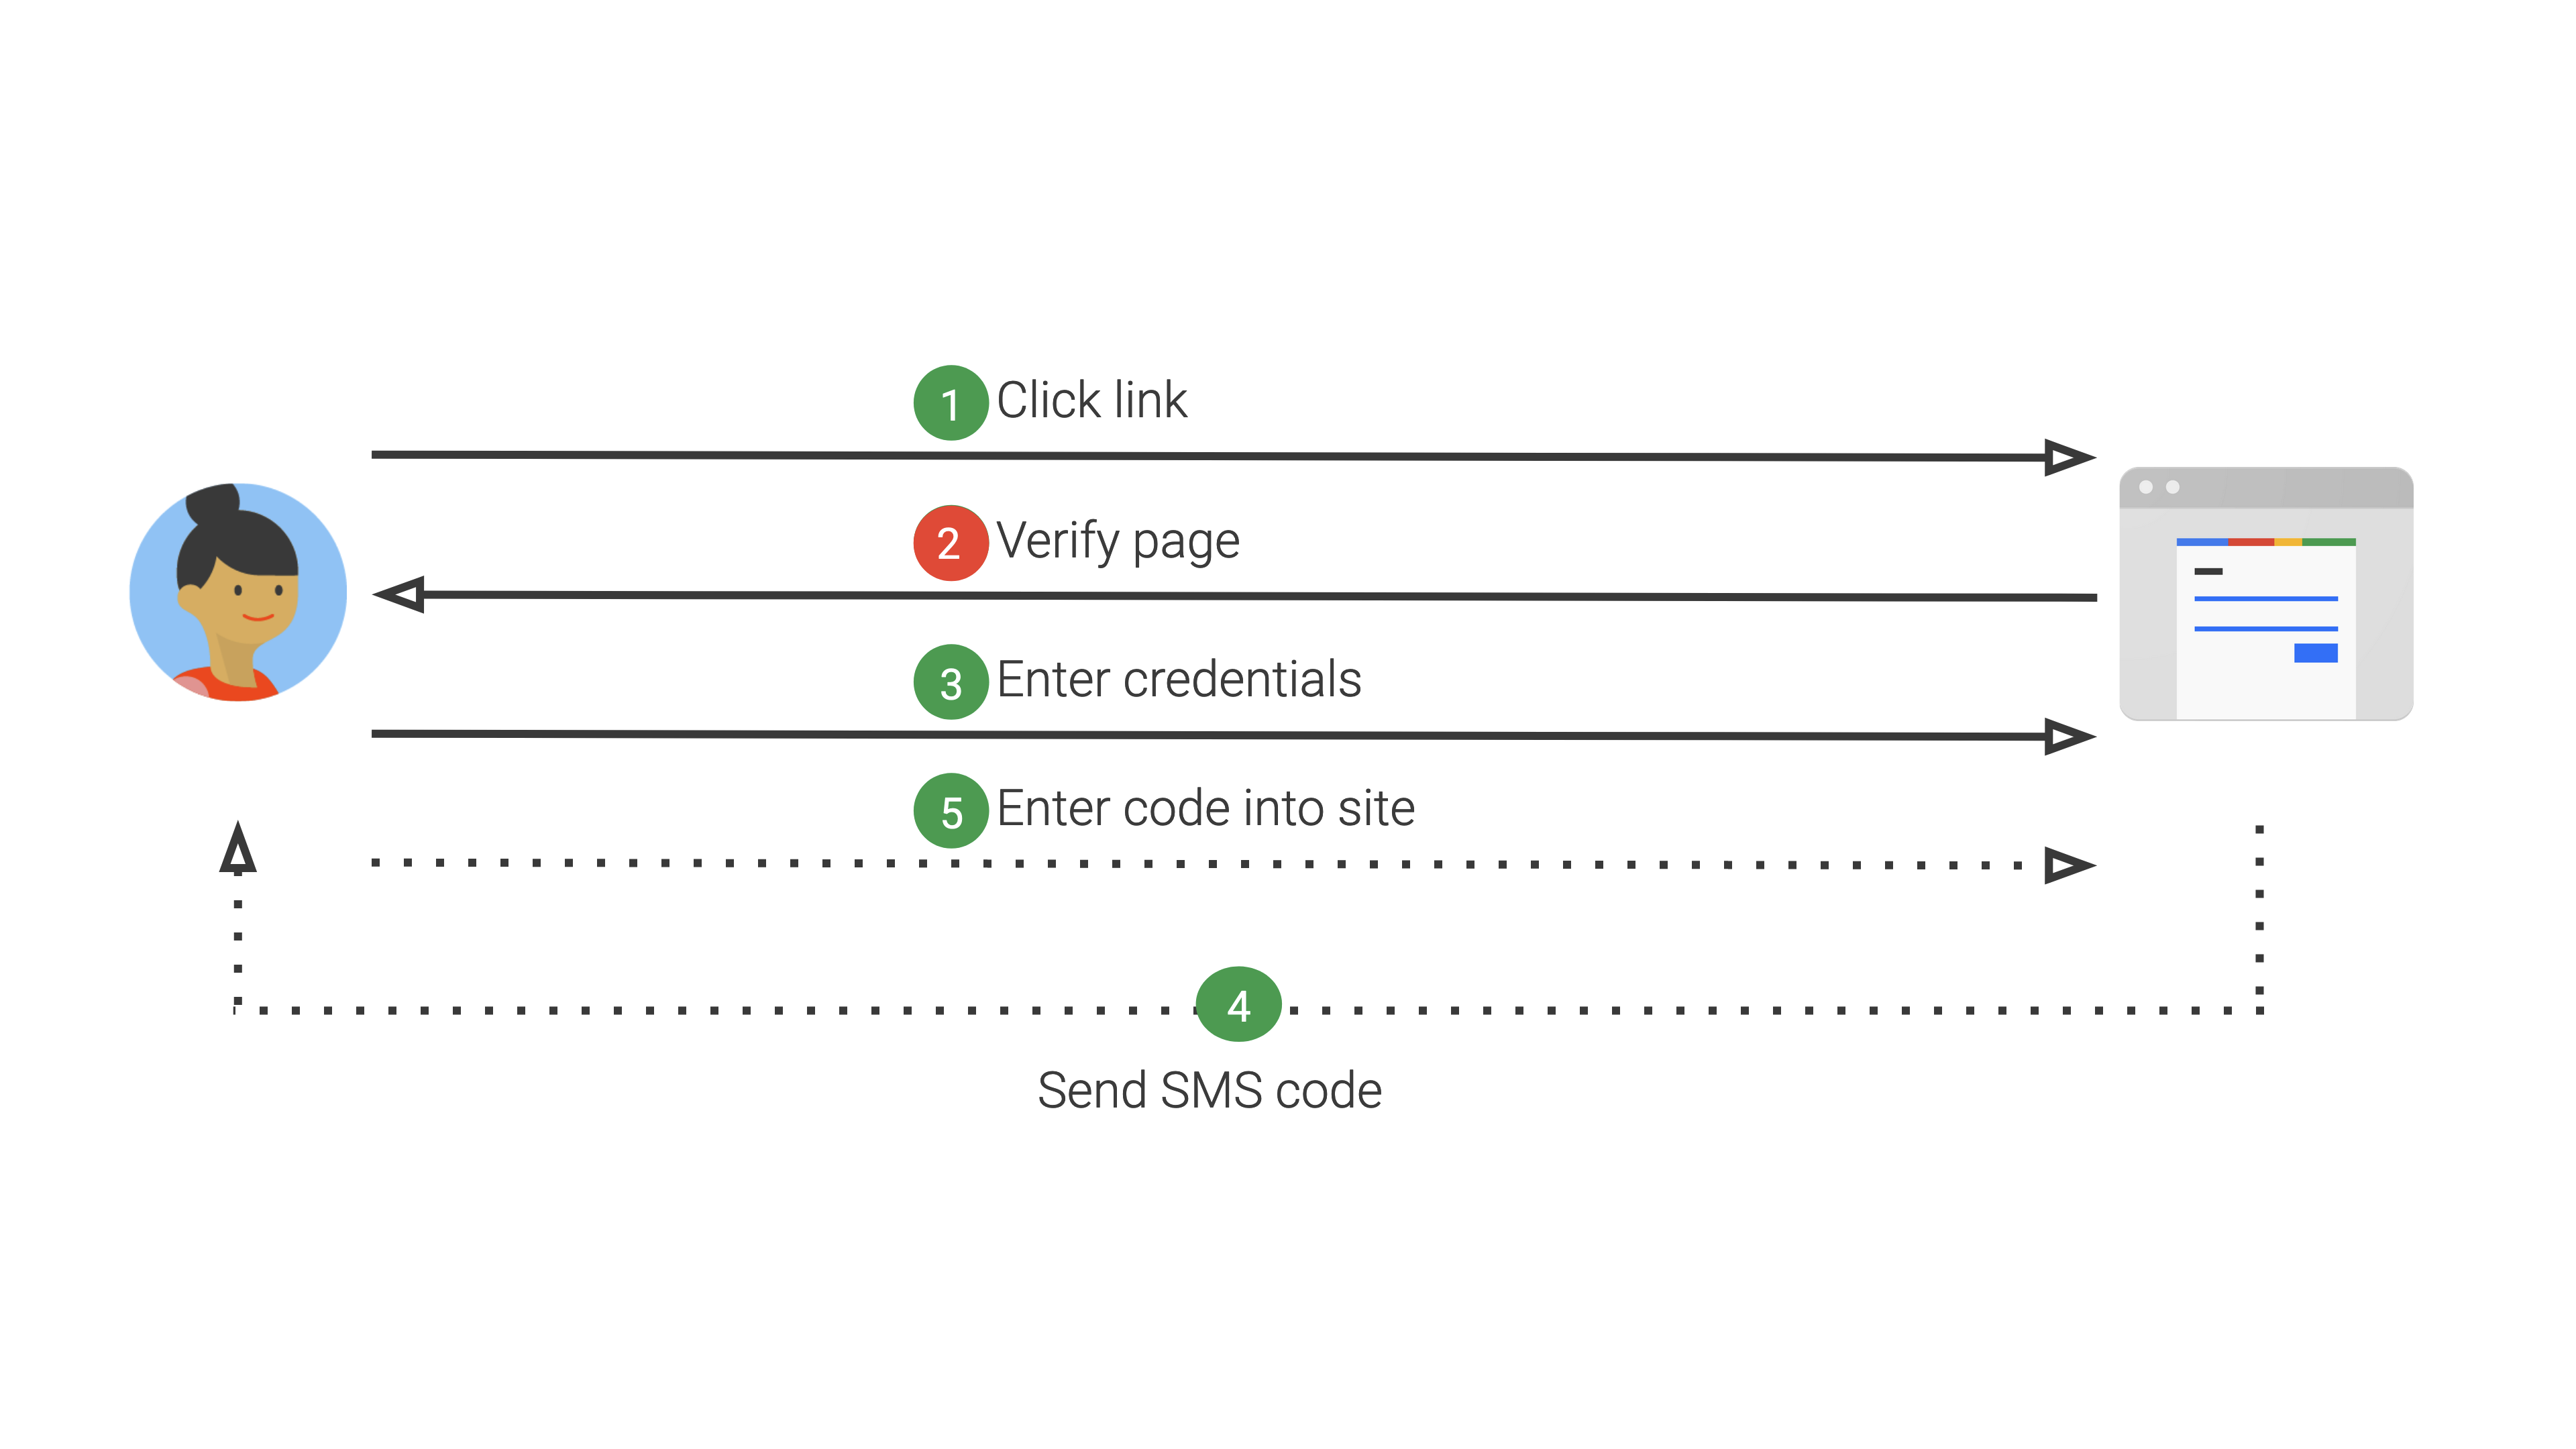
\includegraphics[width=\paperwidth]{login-diagram}
\end{frame}

\begin{frame}{}%TODO
    \thispagestyle{empty}
    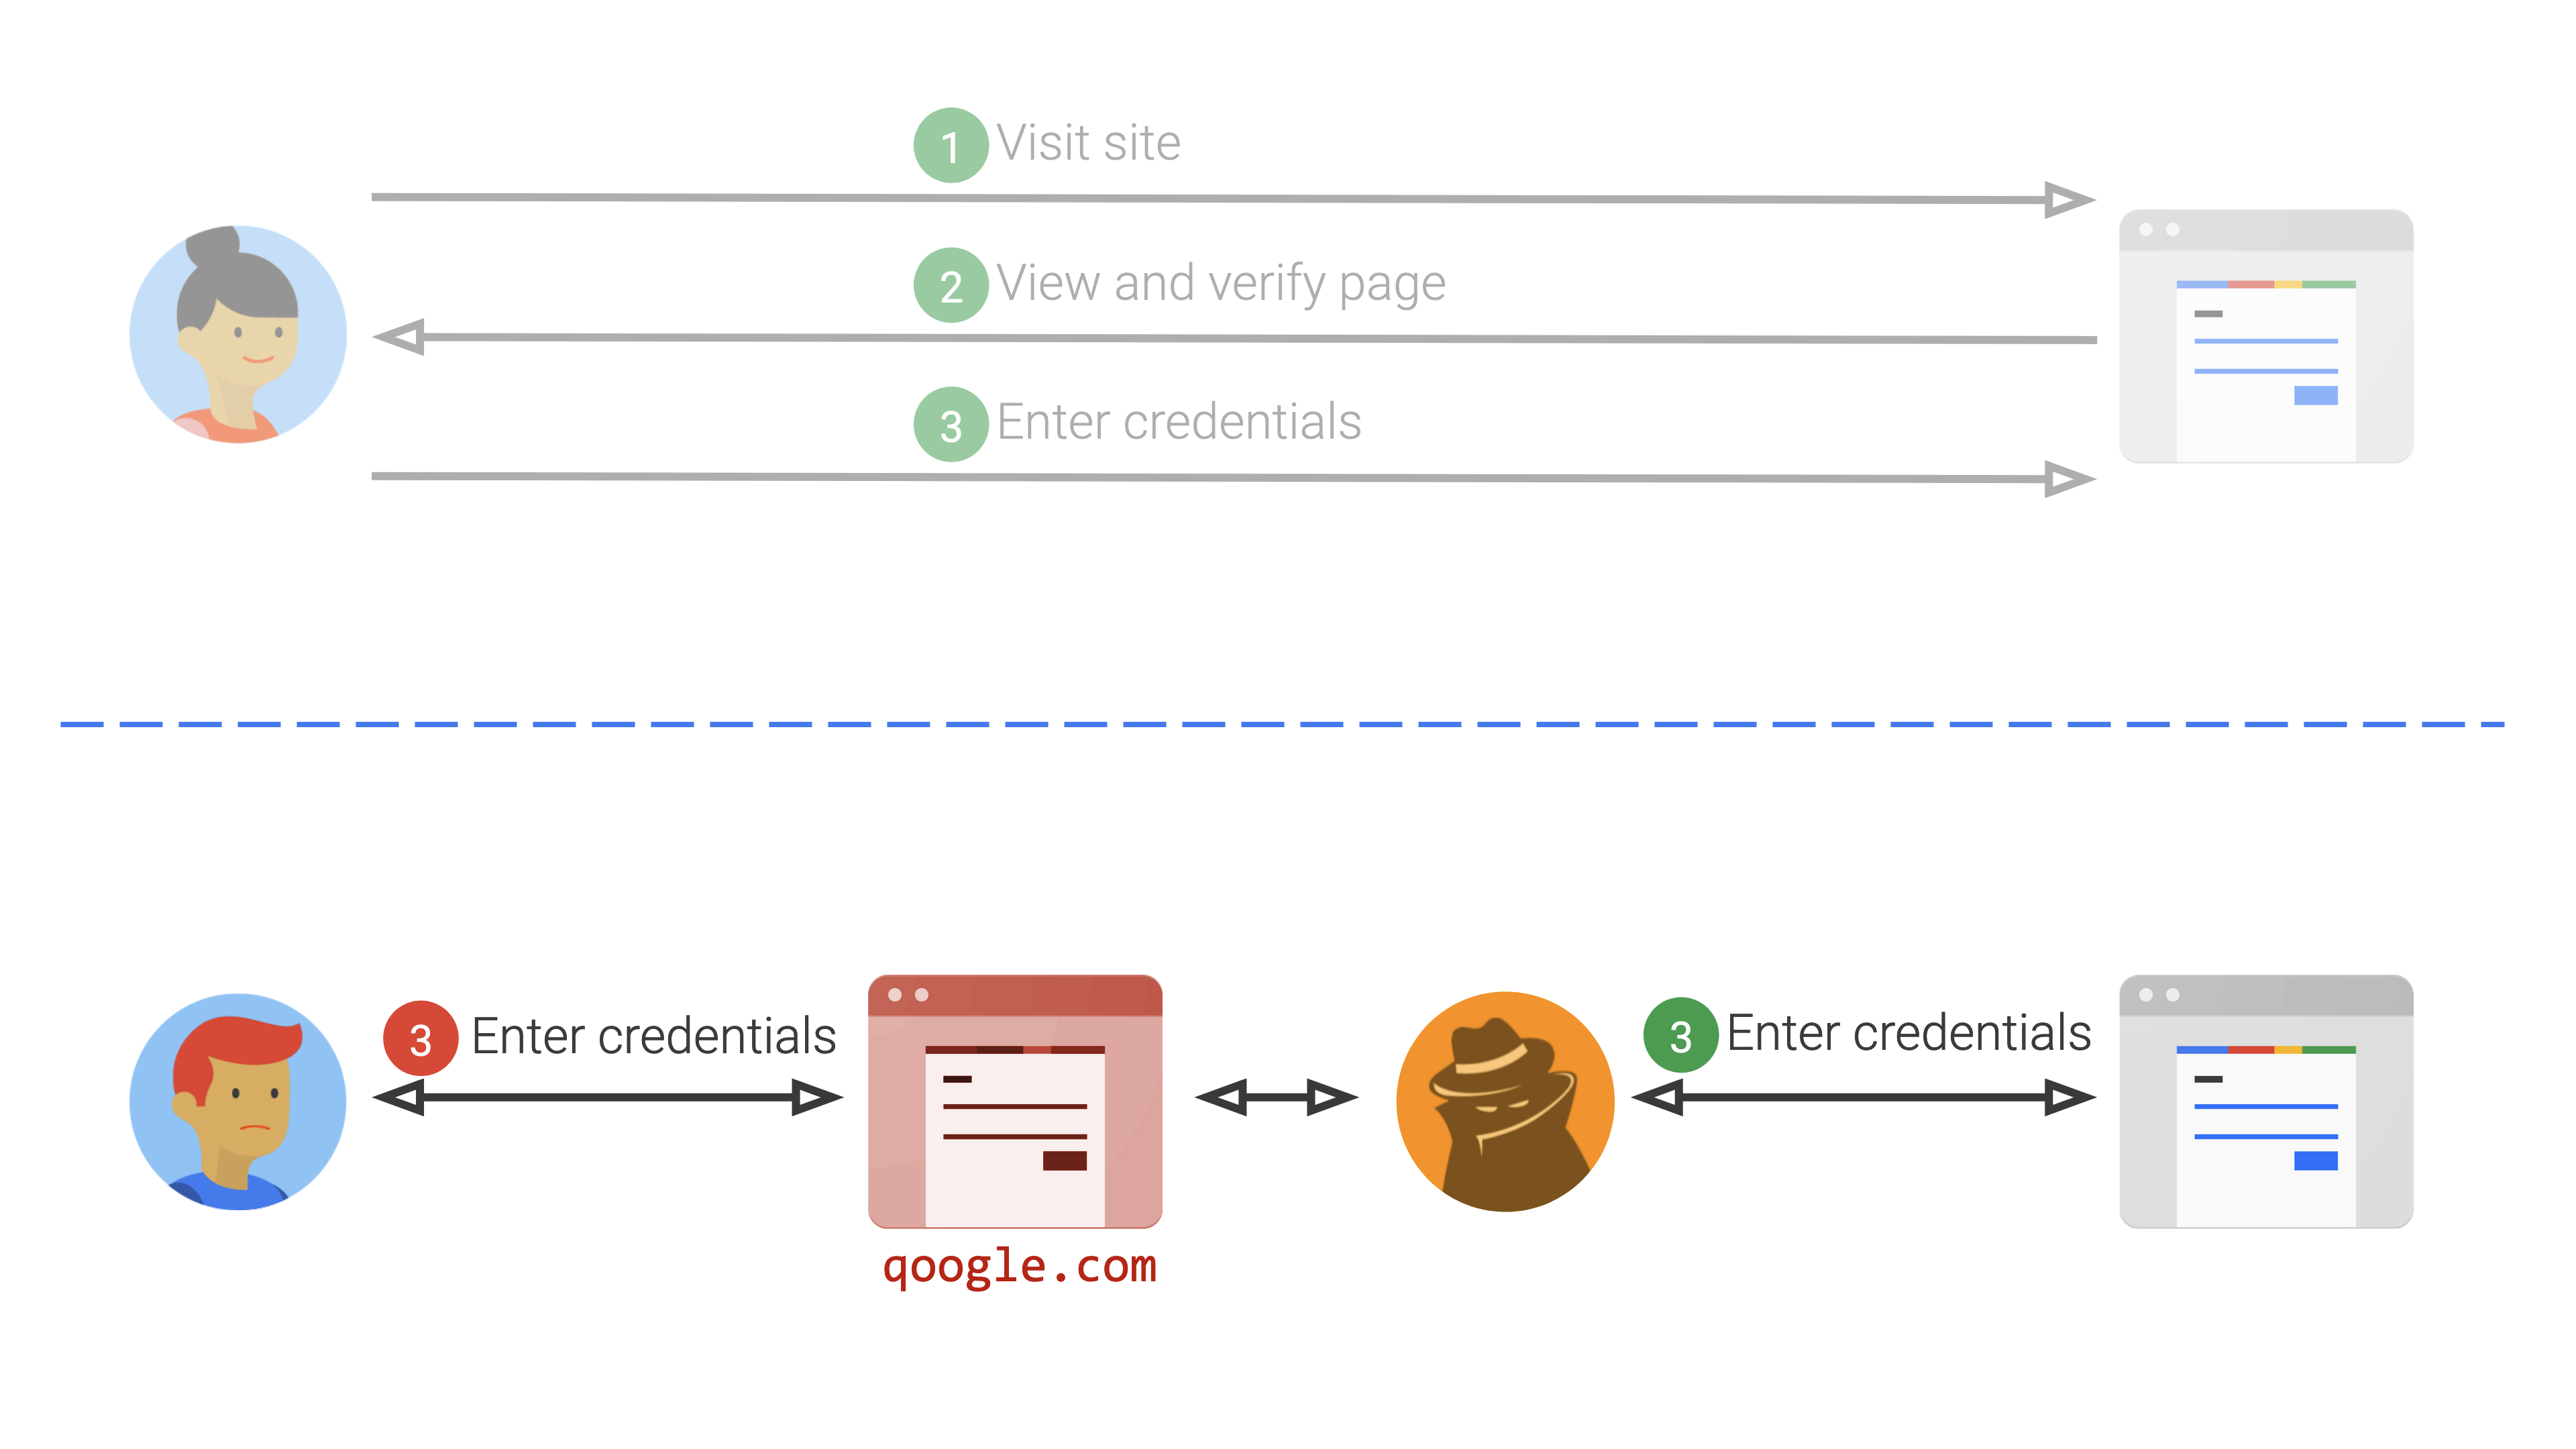
\includegraphics[width=\paperwidth]{login-diagram-phishing}
\end{frame}

\begin{frame}{}%TODO3
    \thispagestyle{empty}
    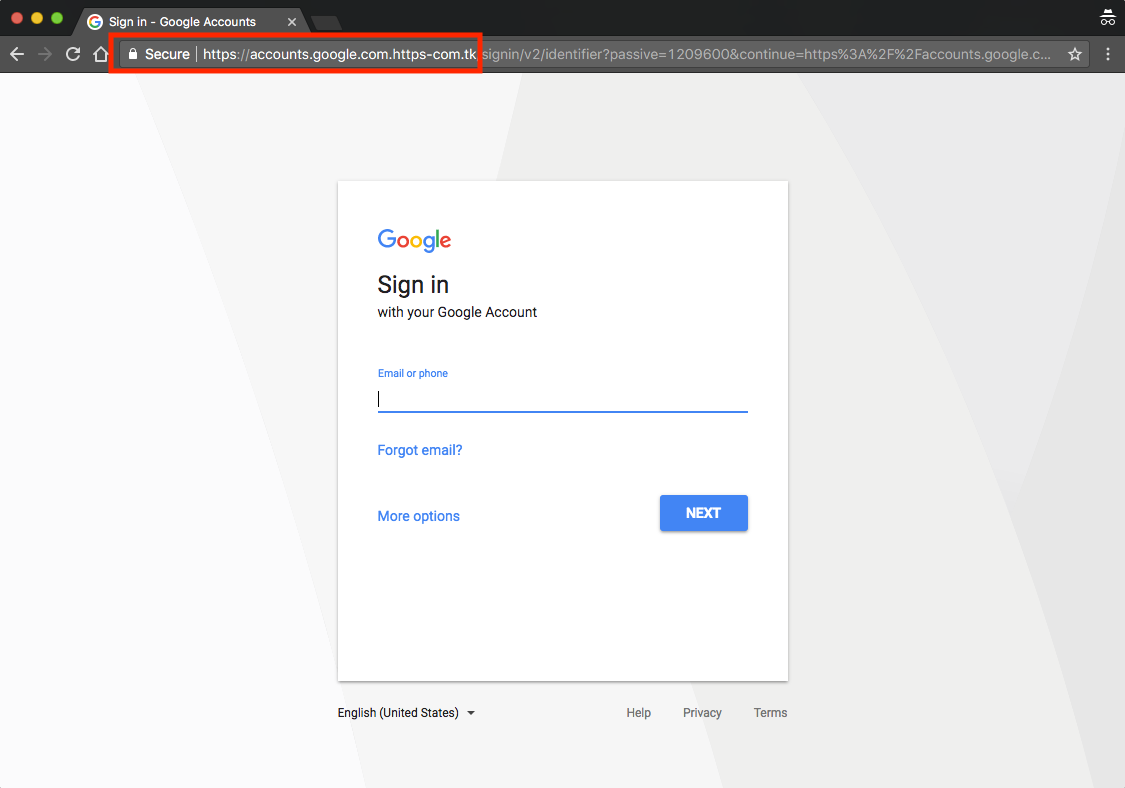
\includegraphics[width=\paperwidth]{bad-link-browser}
\end{frame}

\begin{frame}{}%TODO3 fix
    \thispagestyle{empty}
    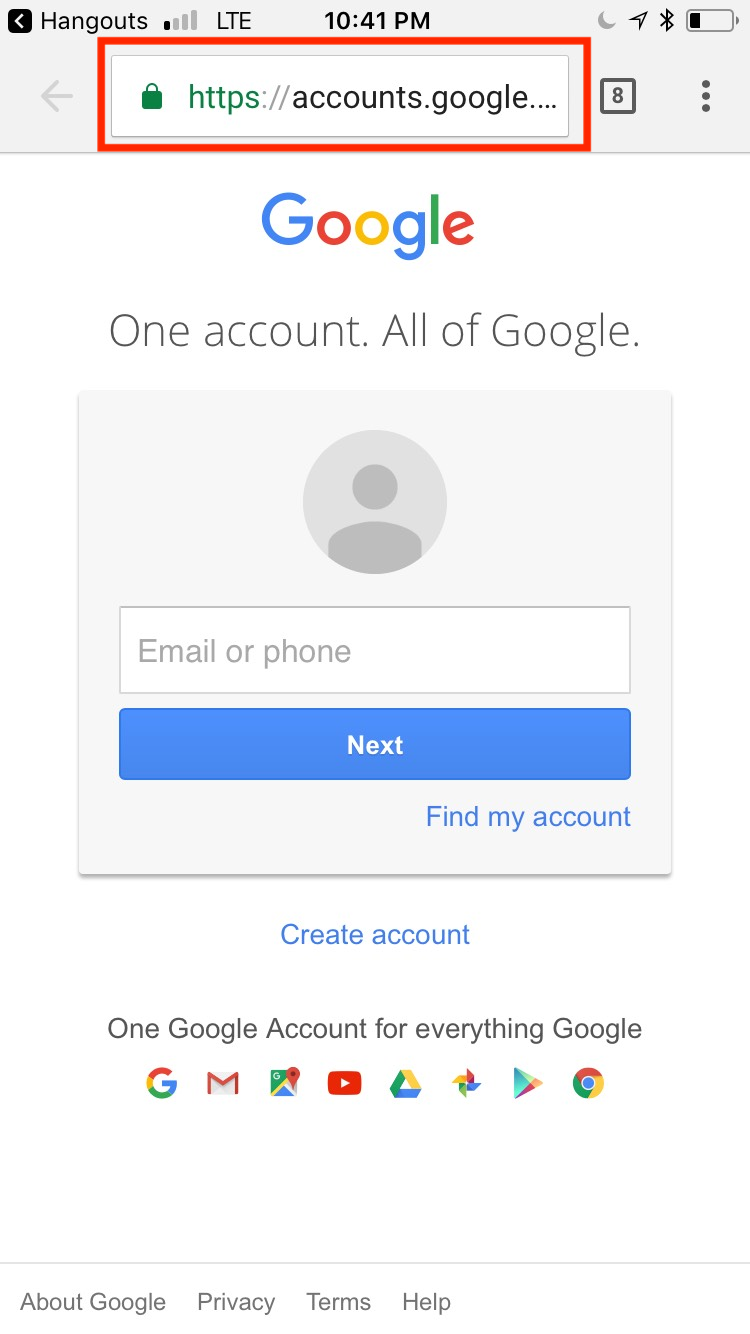
\includegraphics[height=\paperheight]{bad-link-mobile}
\end{frame}

\begin{frame}{}%TODO3 fix - AtPageUpperLeft not doing what eso-pic says it does
    \thispagestyle{empty}
    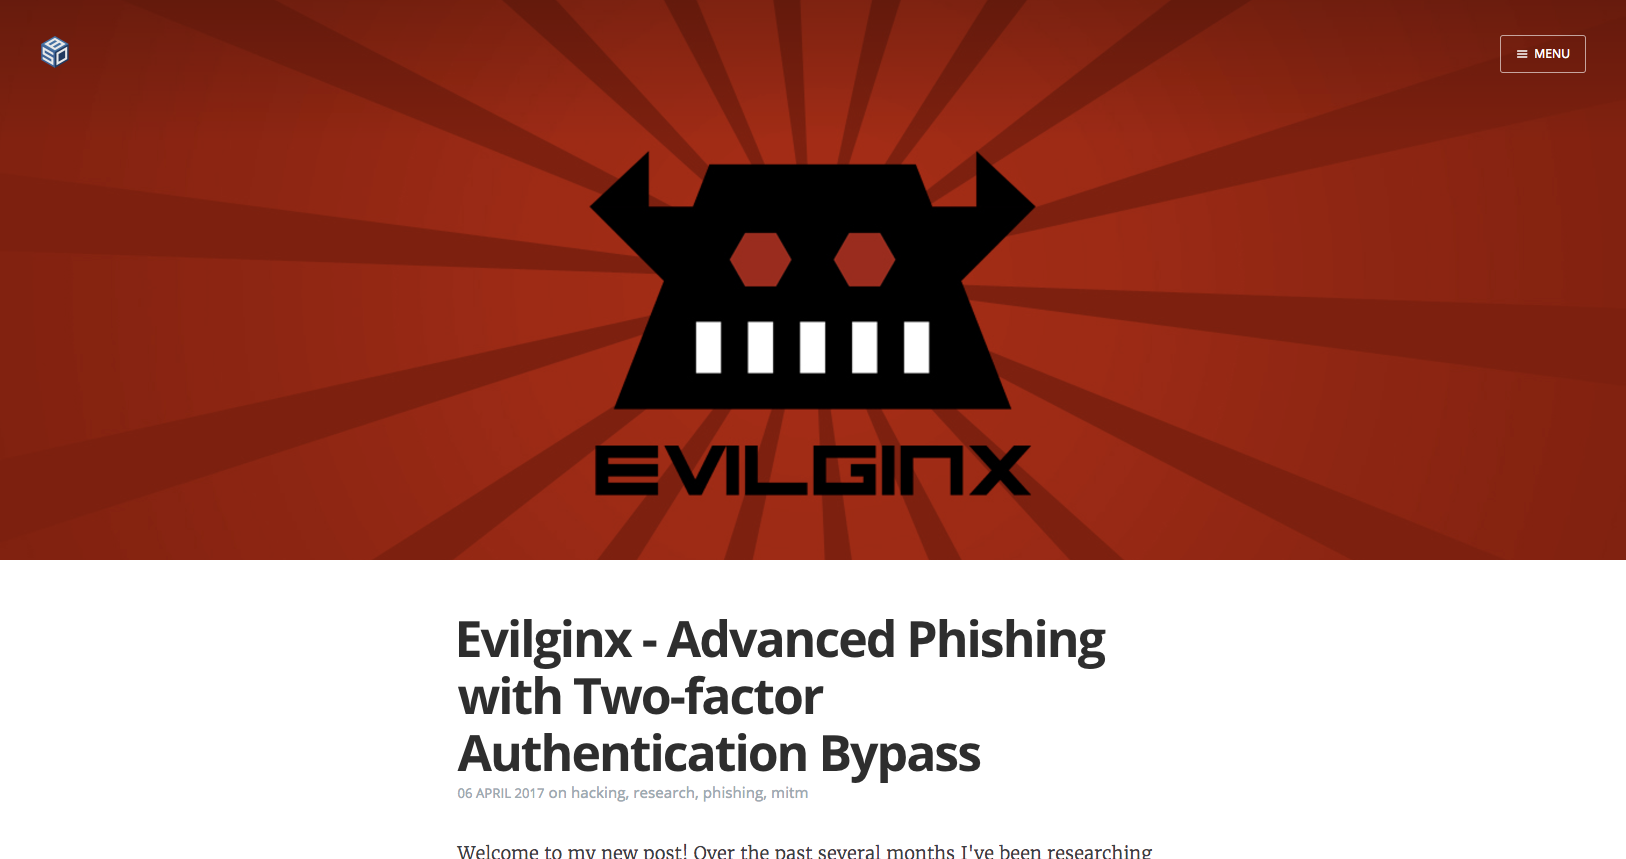
\includegraphics[width=\paperwidth]{evilginx}
\end{frame}

\section{Mitigation}

\begin{frame}{Mitigation}
    \Large
    \begin{itemize}
        \item Risk-based authentication challenges
        \item Implicit signals
        \item Strong authentication
        \item Federation
    \end{itemize}
\end{frame}

\begin{frame}{Sign-in Risk Detection}
    \begin{columns}
        \column{0.55\textwidth}
            \small
            \begin{itemize}
                \item Unusual location, device, time, network 
                \item Phishing history
                \item Similarity to known account hijacking patterns (number of login attempts, sensitivity of info accessed, etc.)
                \item \textit{The higher the estimated probability that the login attempt is fraudulent, the more multi-factor authentication steps should be required of the user.}
            \end{itemize}
            \centering
            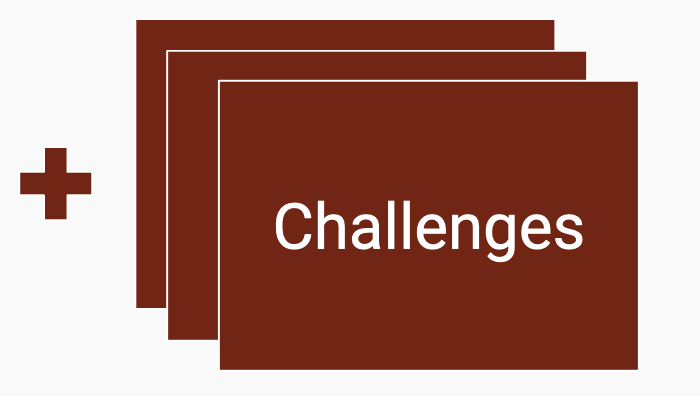
\includegraphics[width=0.6\textwidth]{challenges}
        \column{0.45\textwidth}
            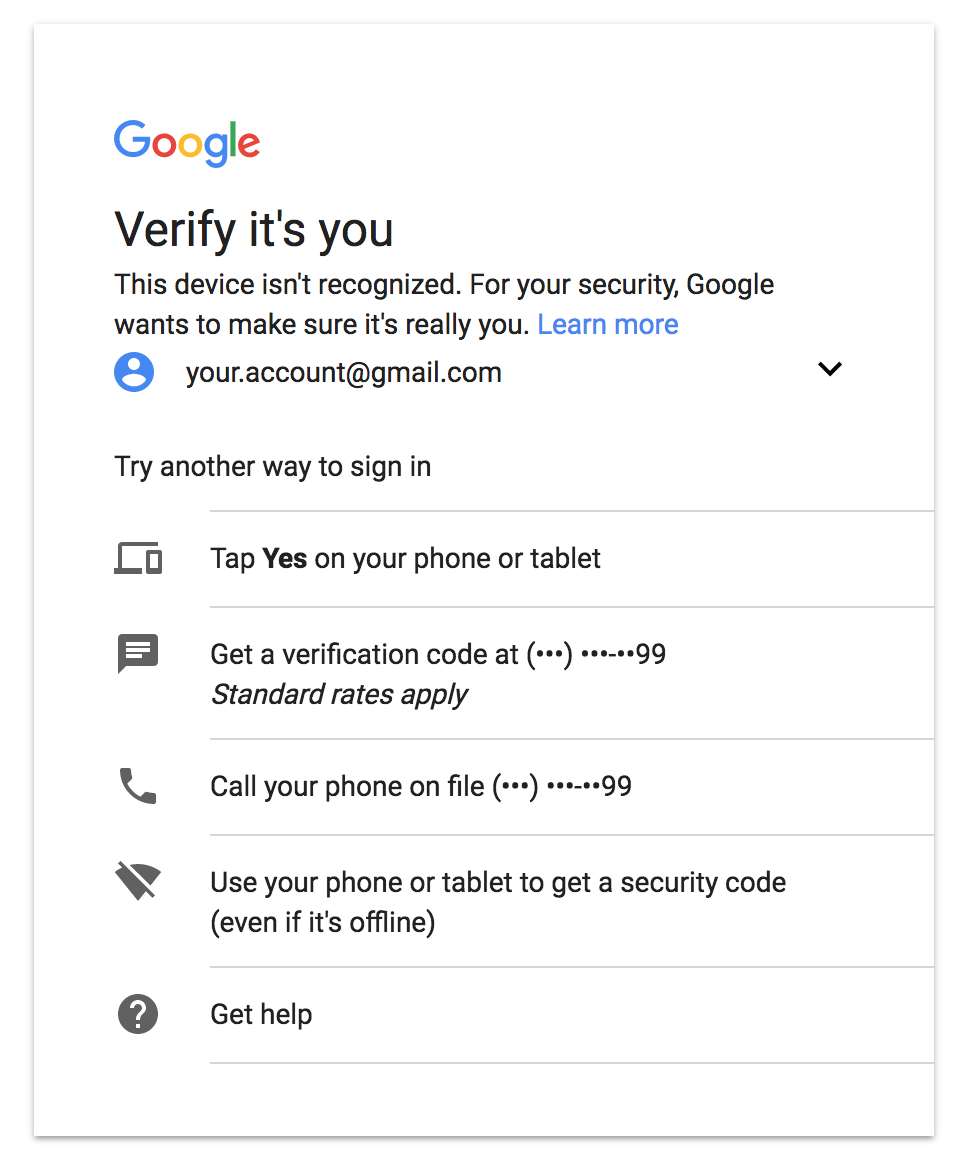
\includegraphics[width=\textwidth]{google-2fa}
    \end{columns}
\end{frame}

\begin{frame}{Detecting Hijacker In-session}
    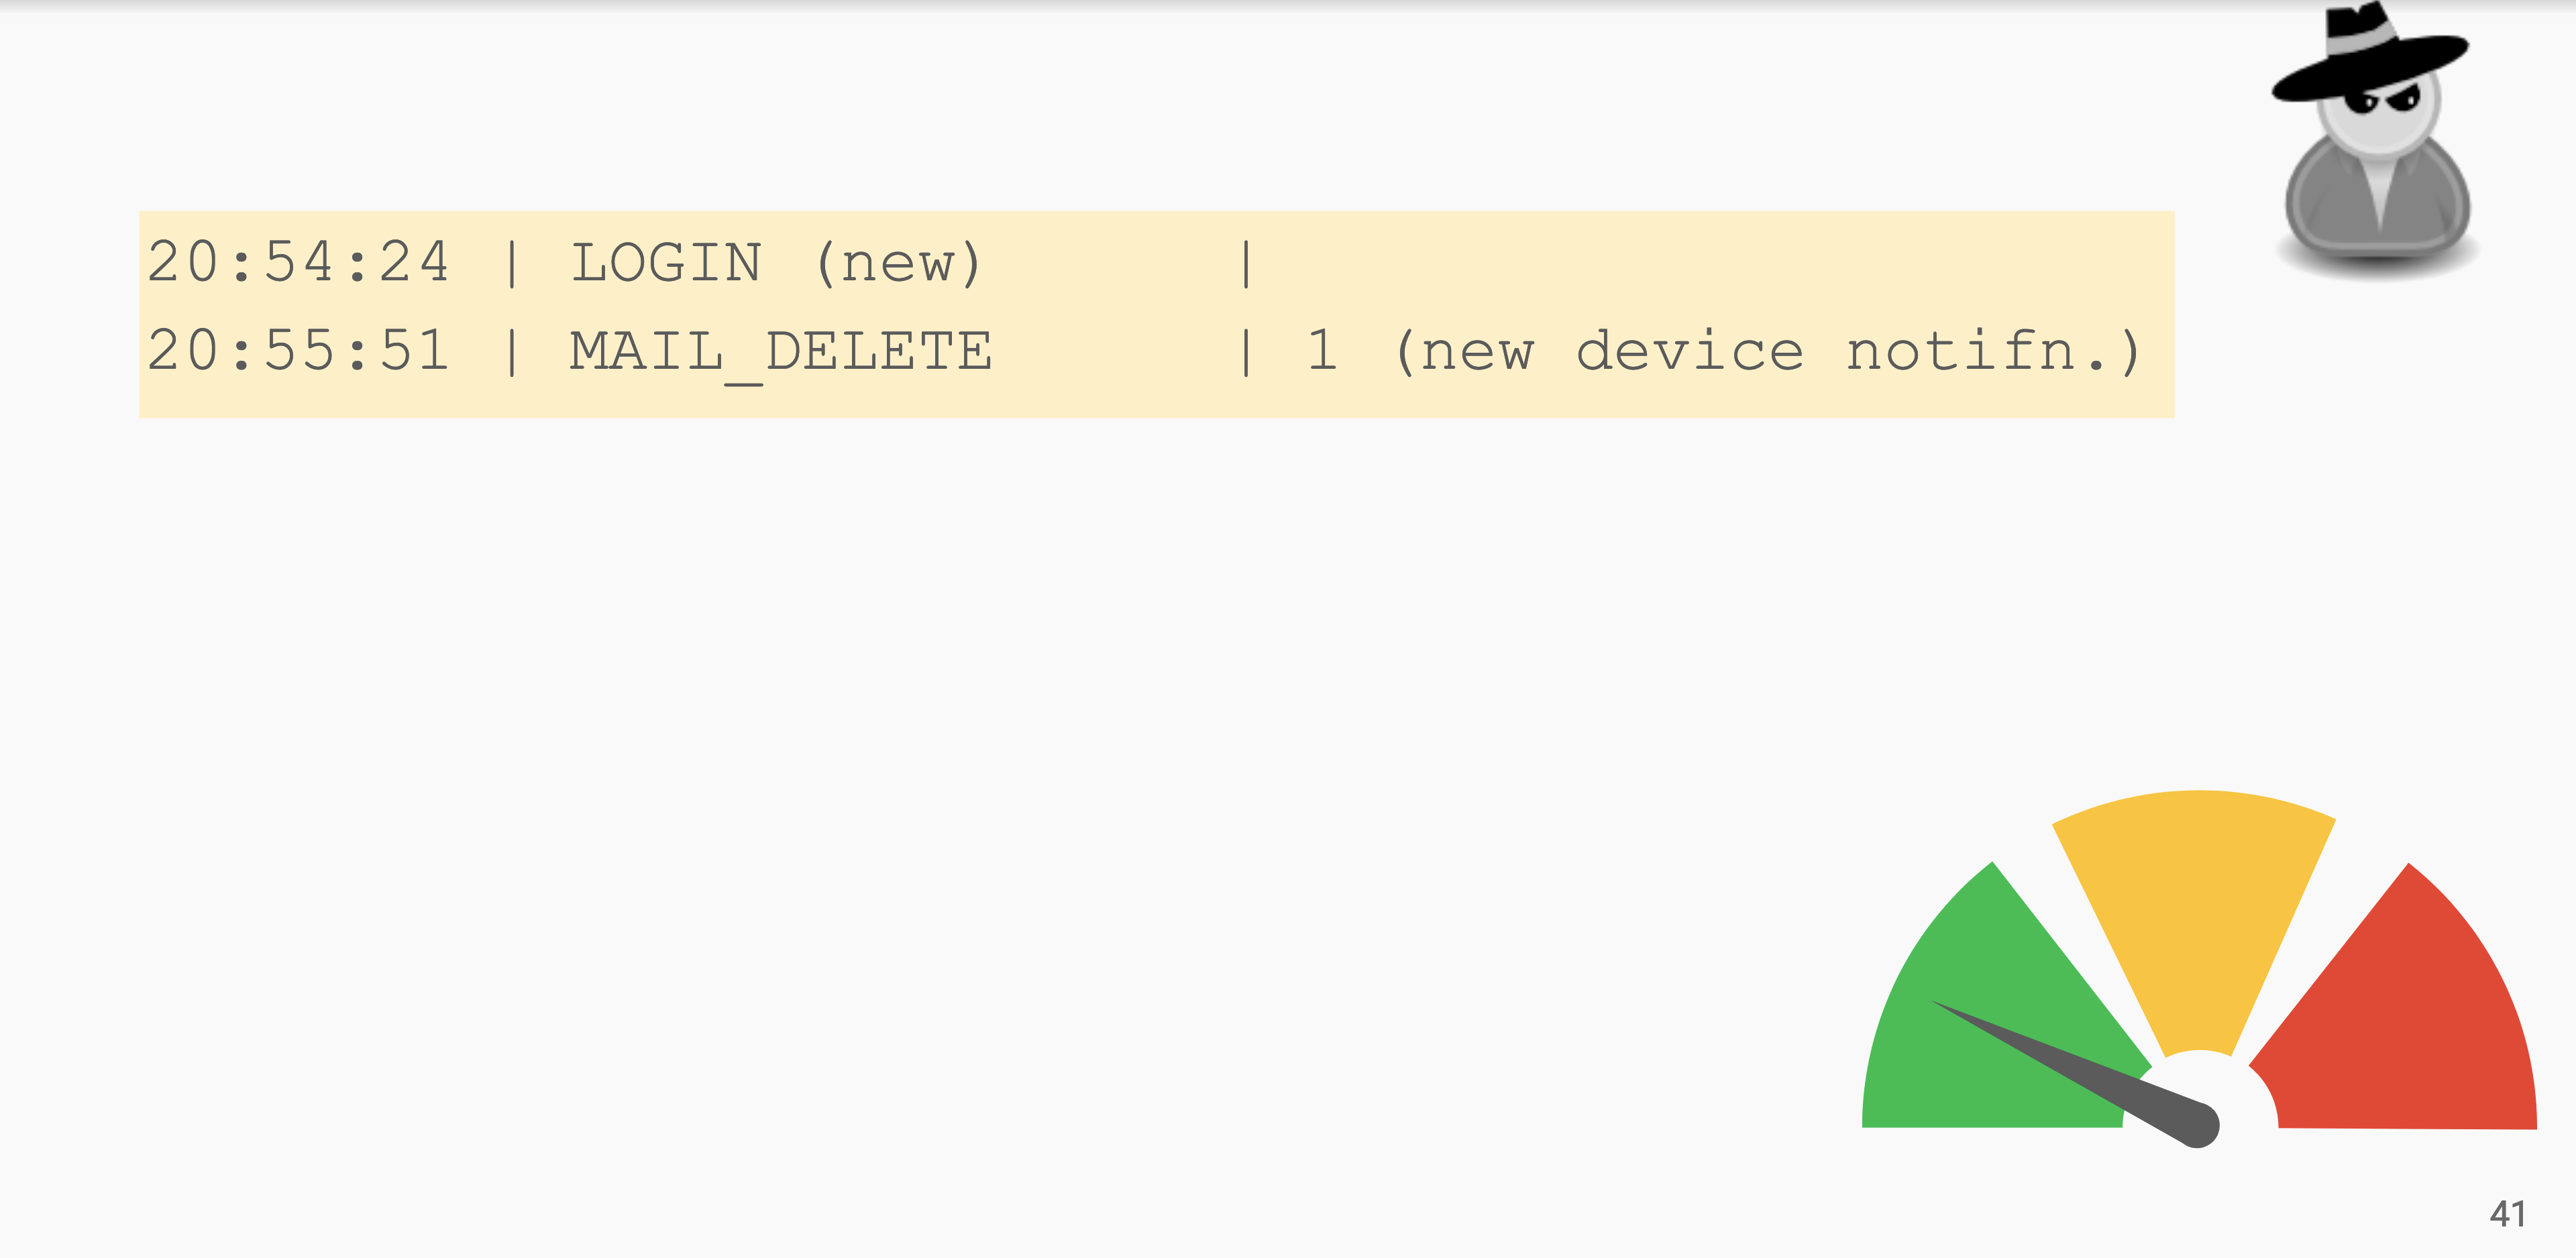
\includegraphics[width=\textwidth]{detecting-hijackers-1}
\end{frame}

\begin{frame}{Detecting Hijacker In-session}
    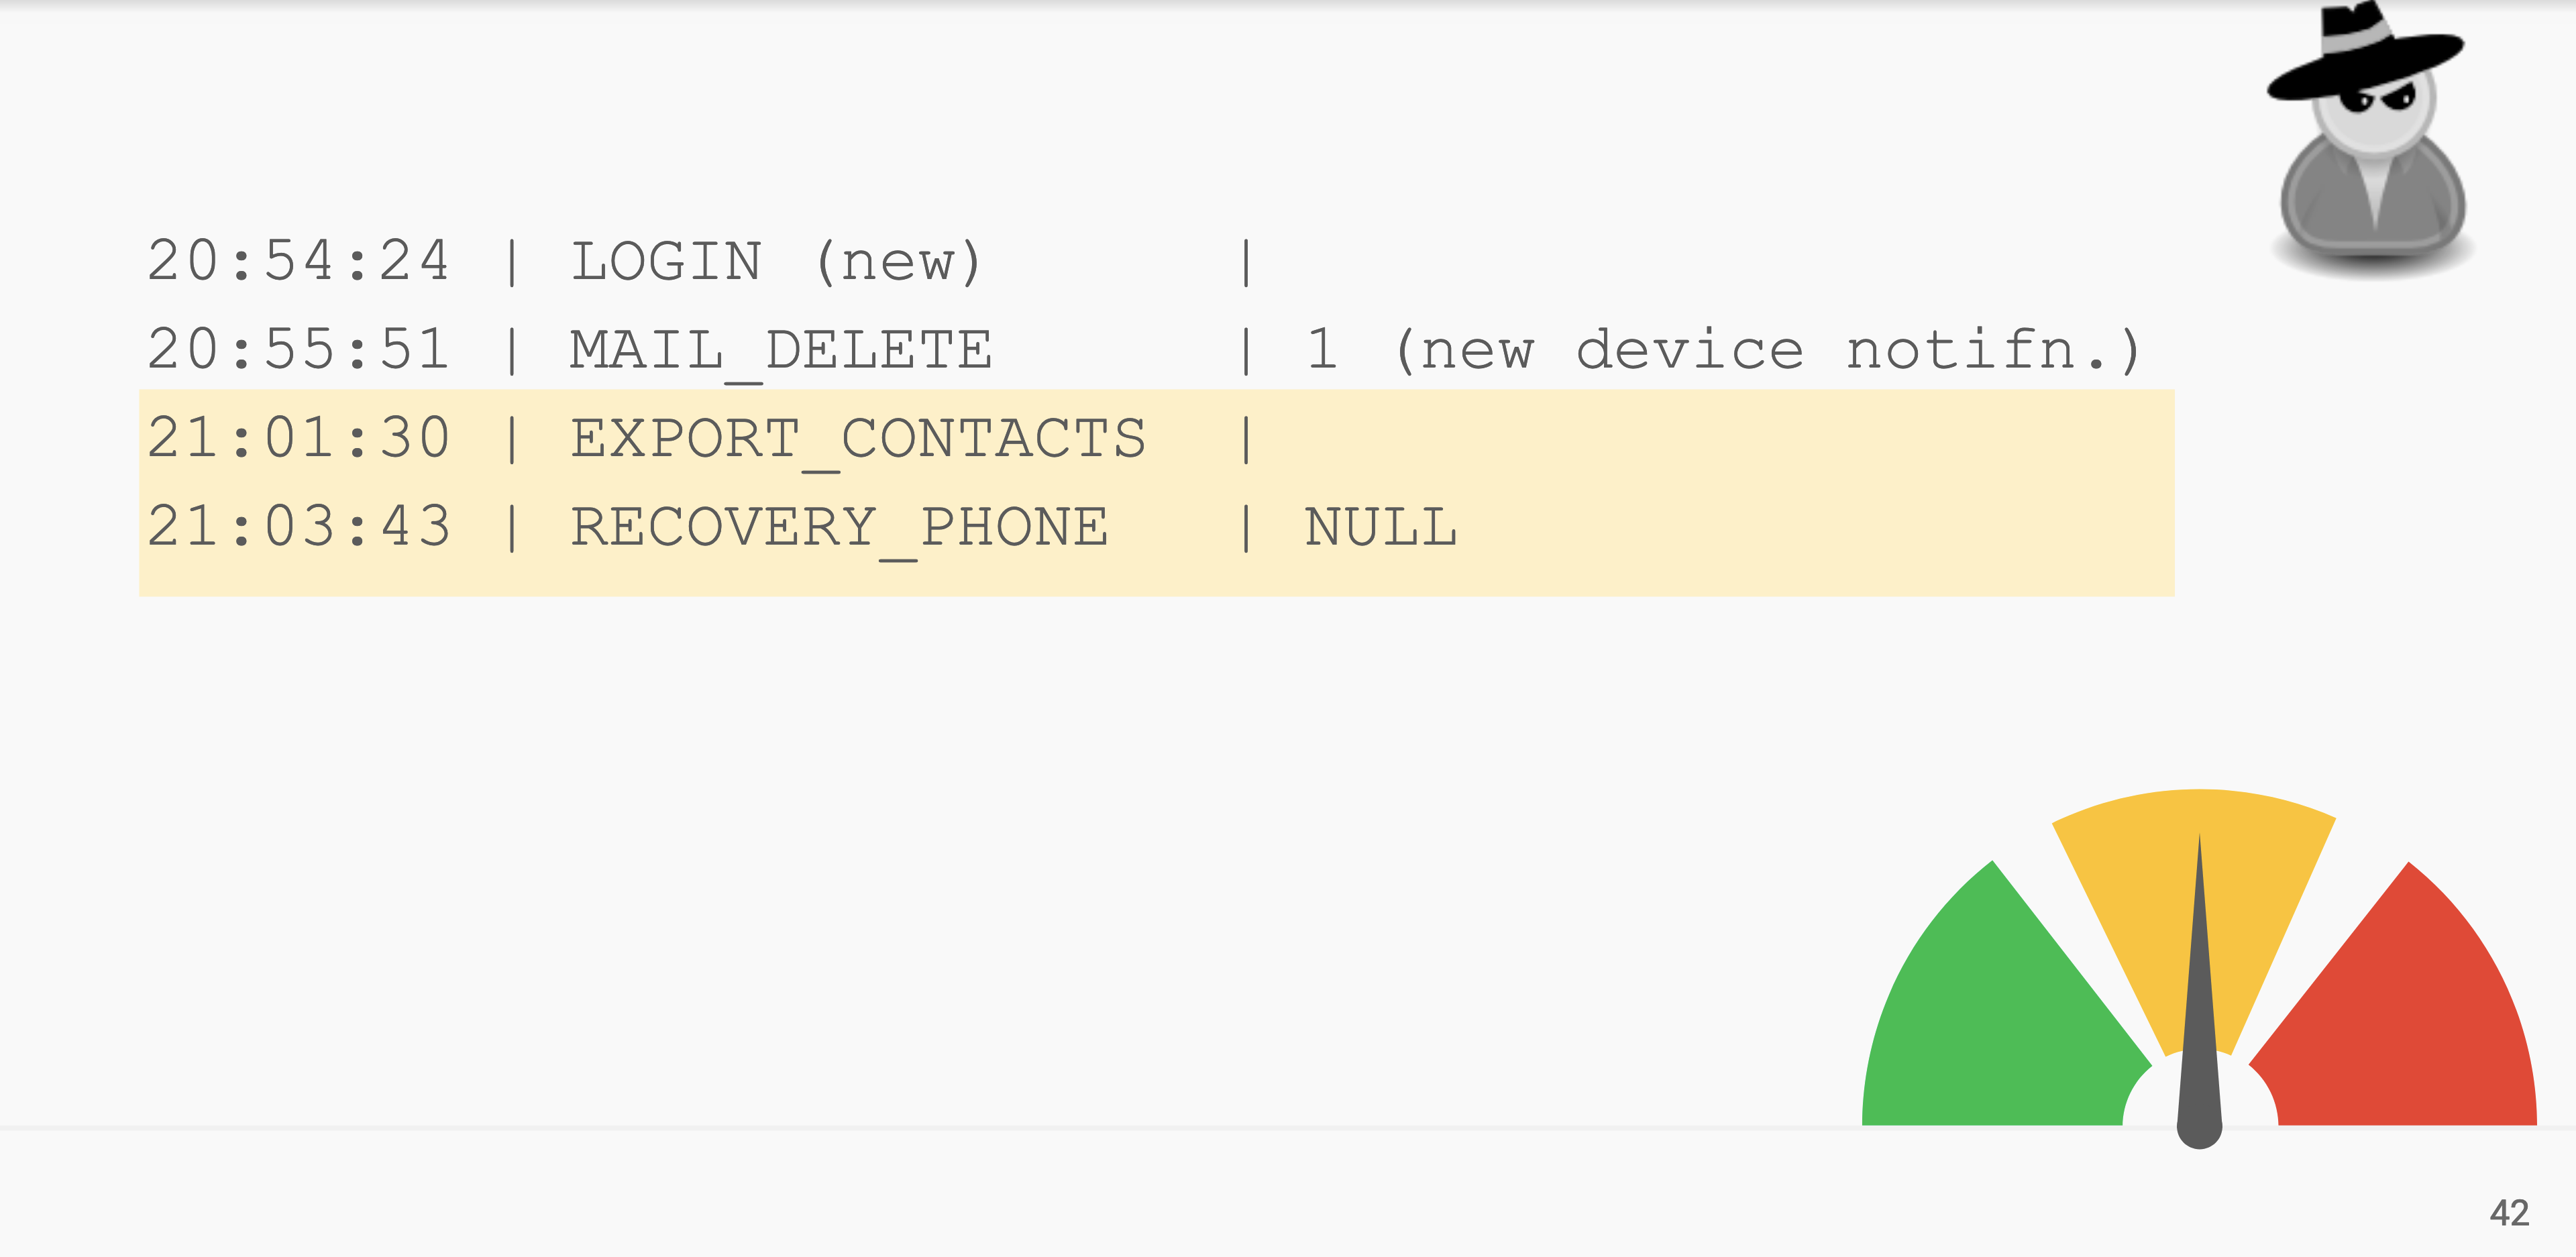
\includegraphics[width=\textwidth]{detecting-hijackers-2}
\end{frame}

\begin{frame}{Detecting Hijacker In-session}
    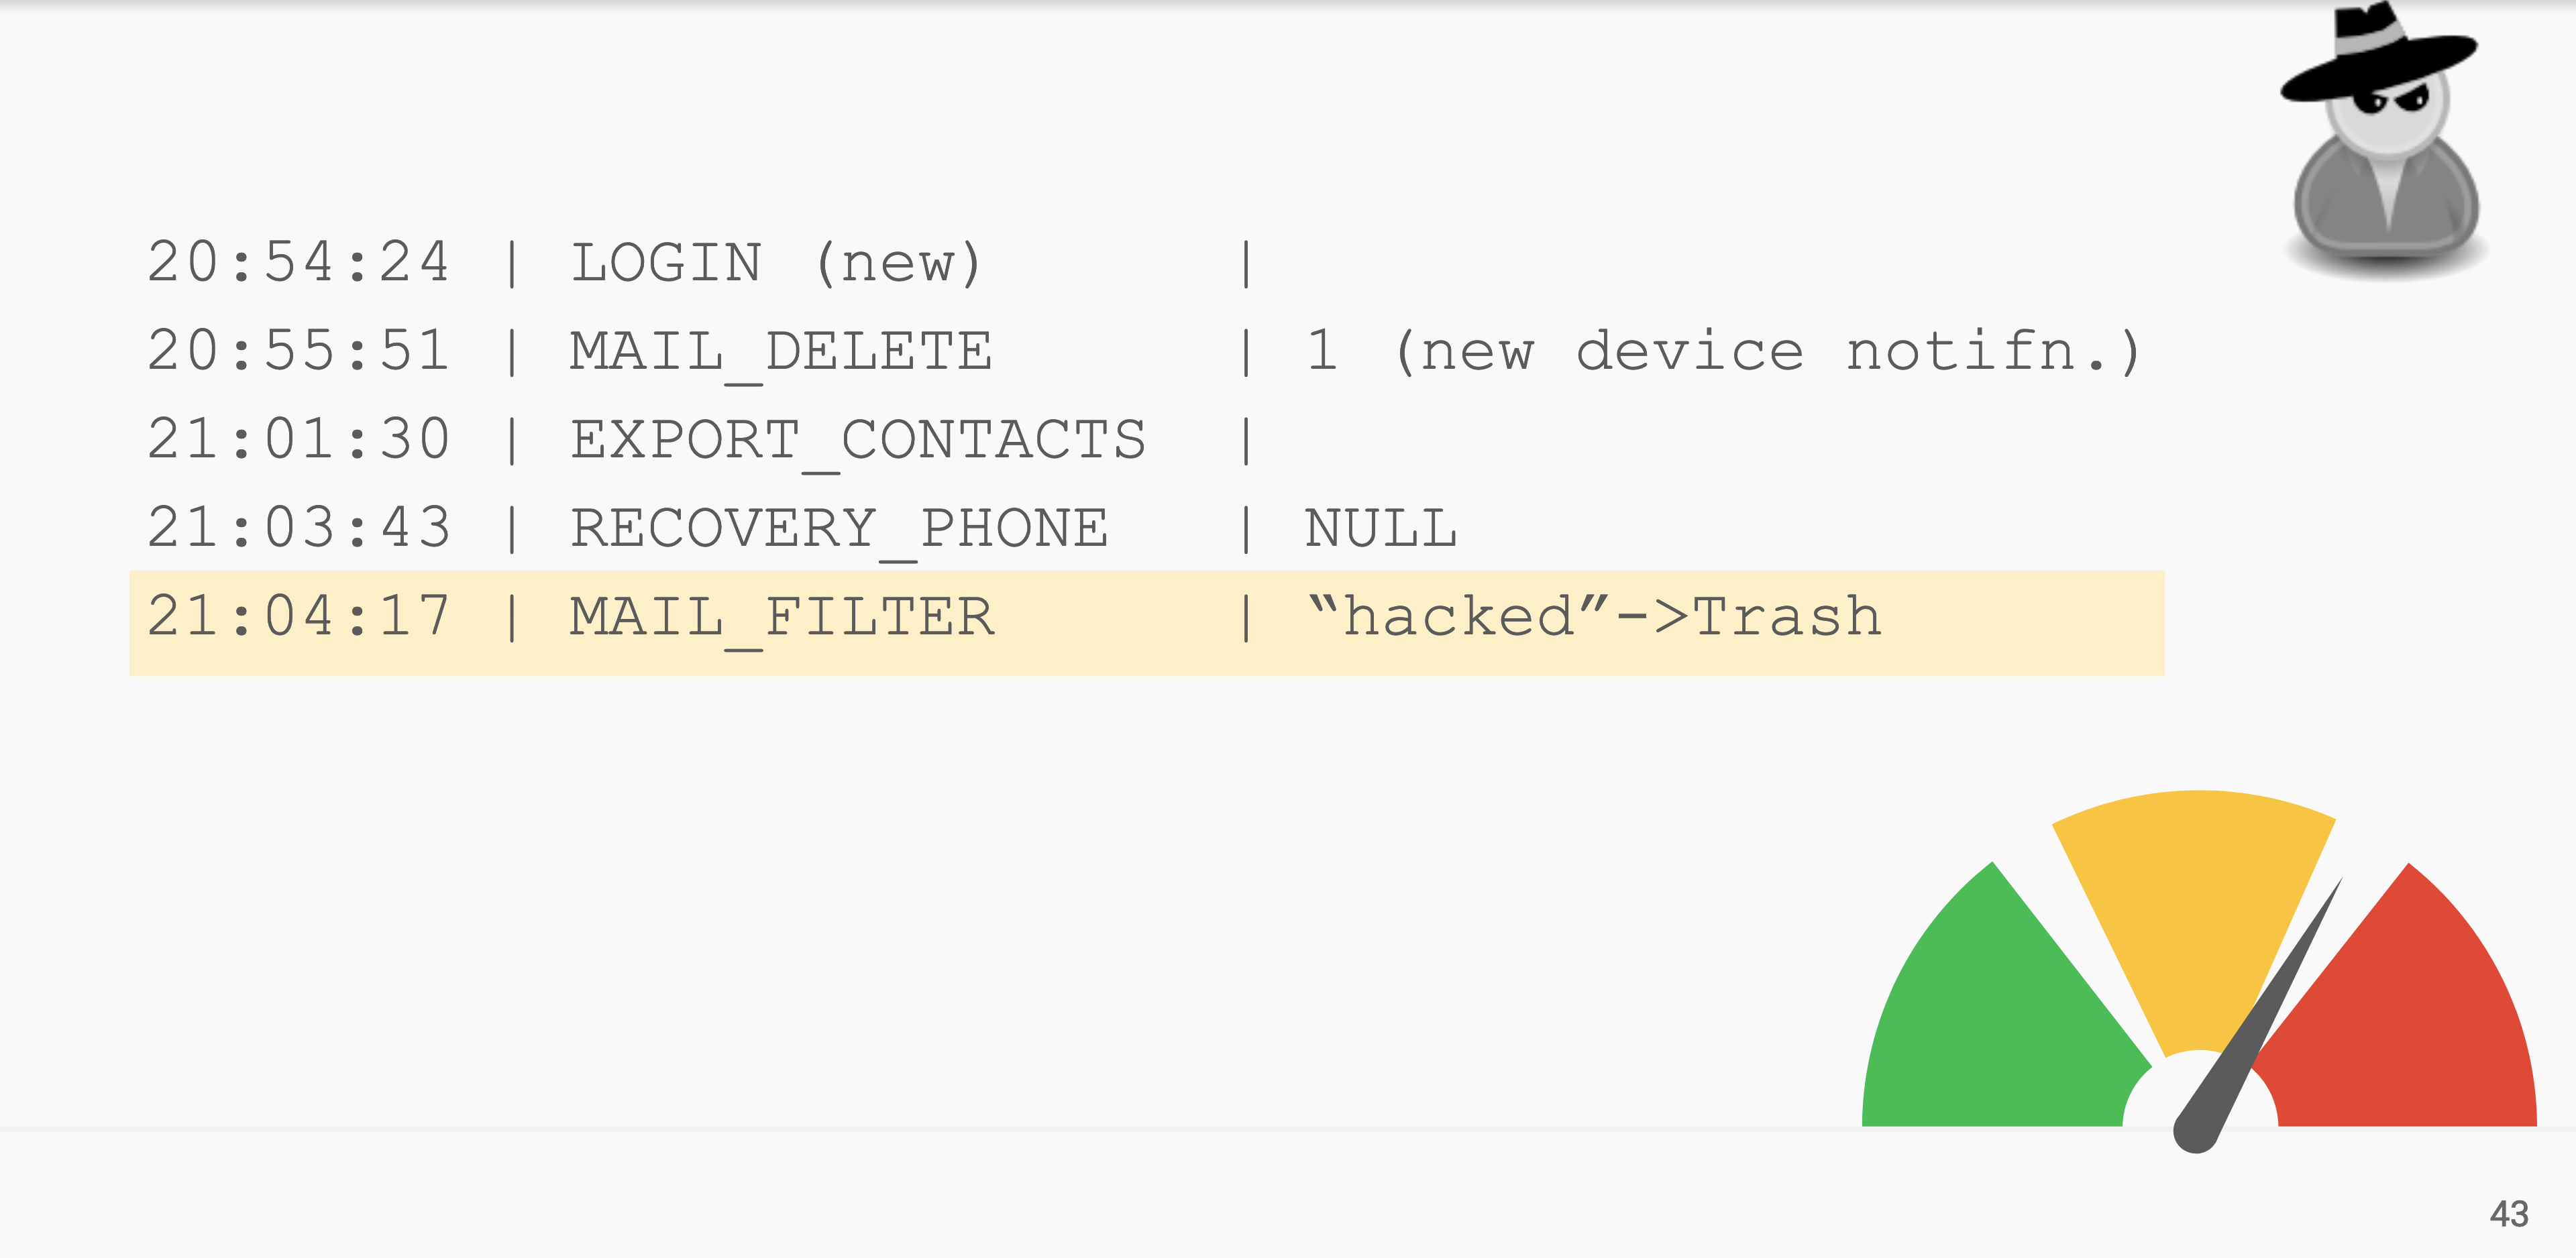
\includegraphics[width=\textwidth]{detecting-hijackers-3}
\end{frame}

\begin{frame}{Detecting Hijacker In-session}
    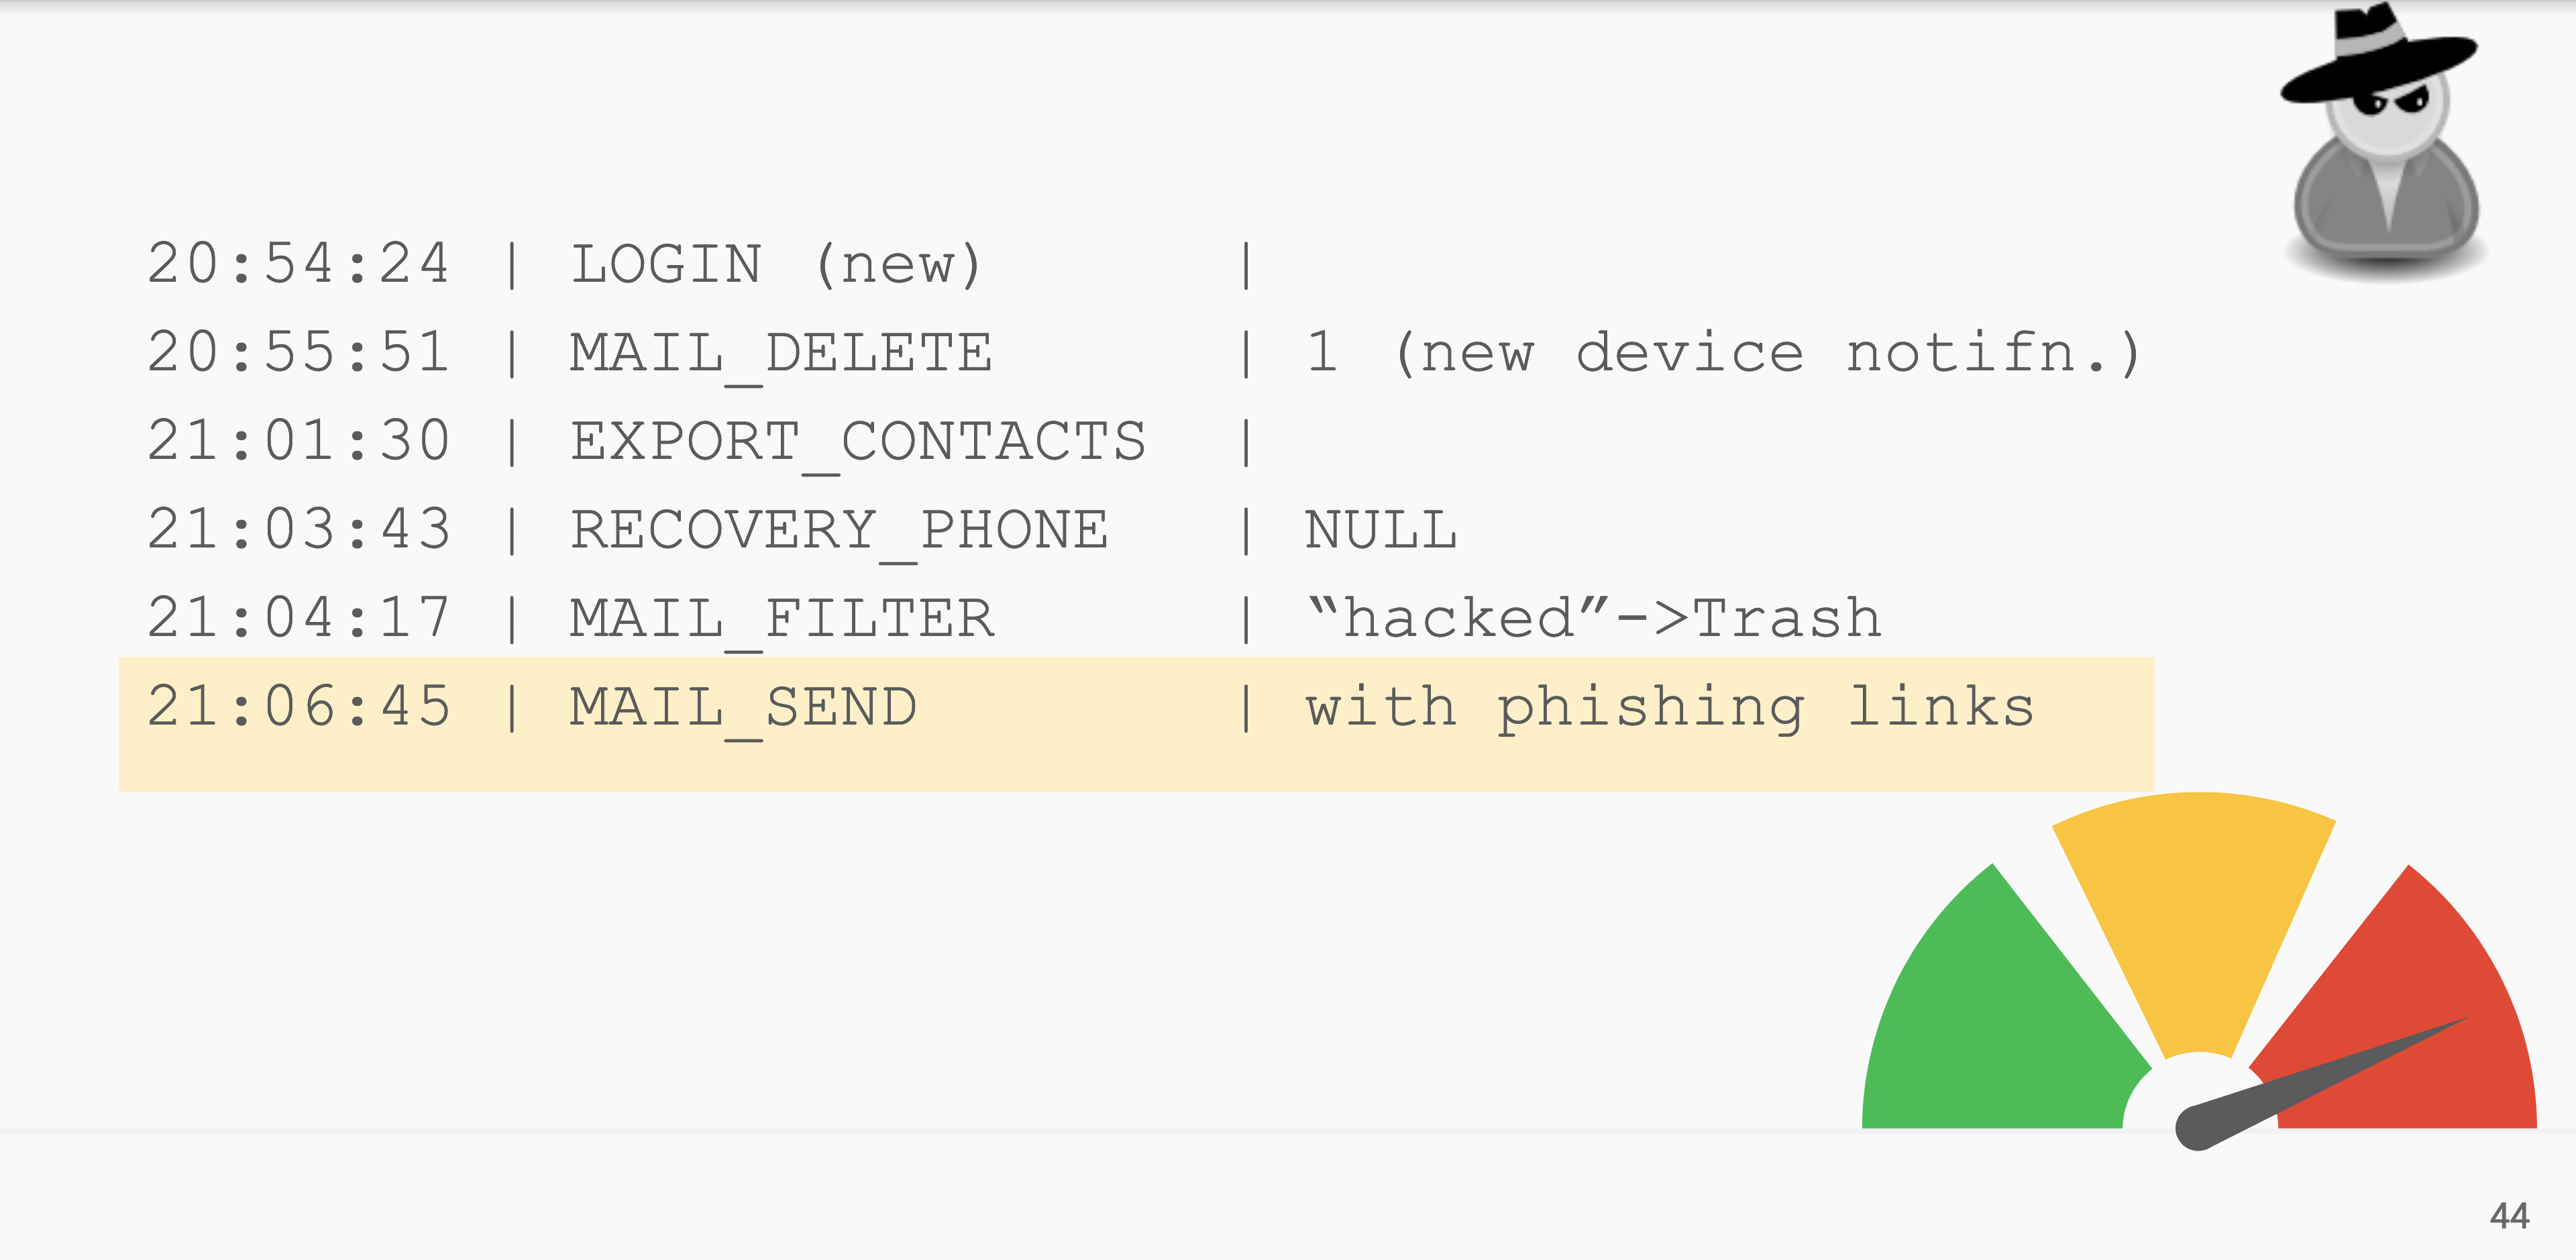
\includegraphics[width=\textwidth]{detecting-hijackers-4}
\end{frame}

\begin{frame}{Authentication Beyond Passwords}
    \centering
    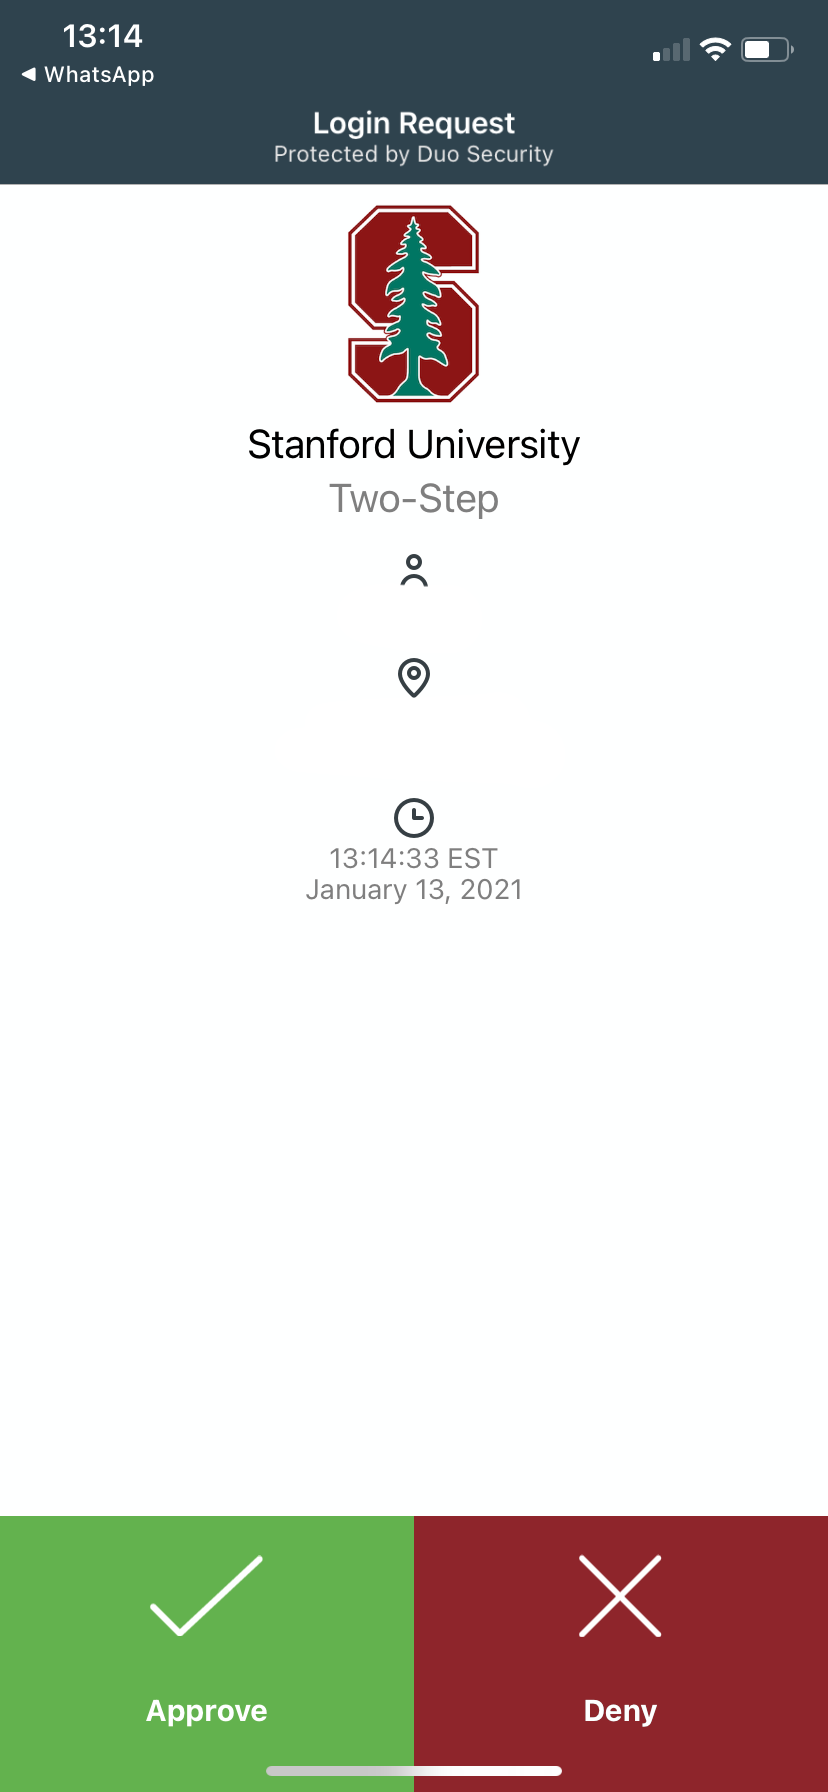
\includegraphics[height=0.86\textheight]{stanford-2fa}
\end{frame}

\begin{frame}{}
    \thispagestyle{empty}
    \AddToShipoutPictureBG*{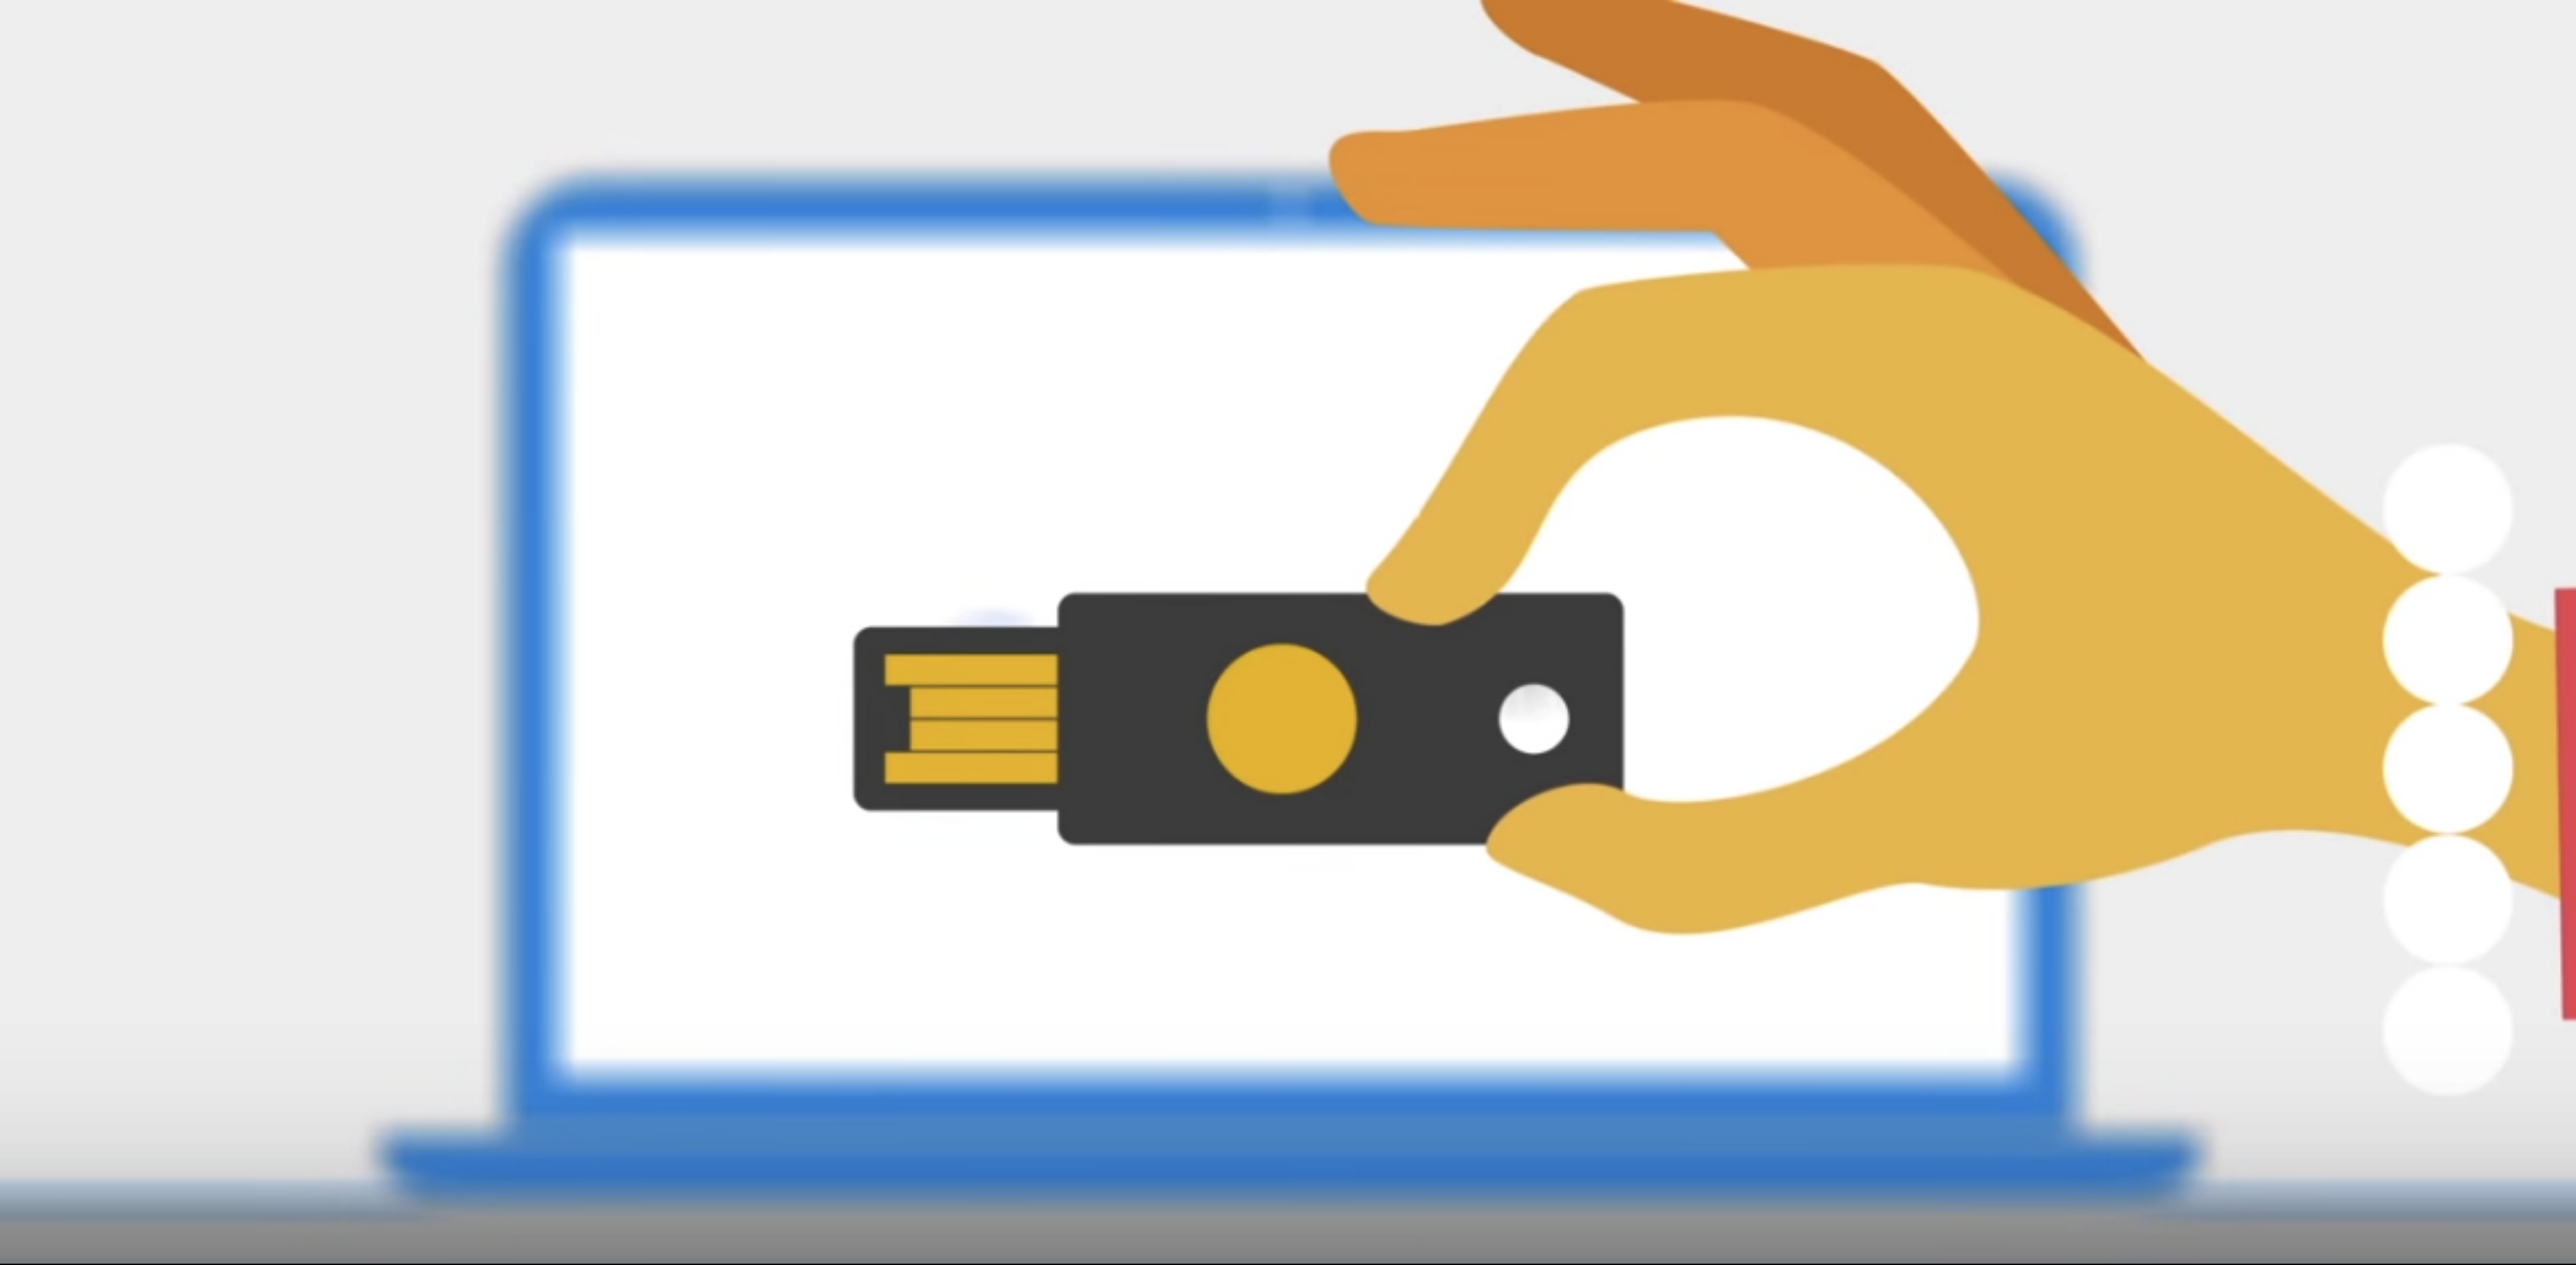
\includegraphics[trim=300 0 0 0, clip, height=\paperheight]{auth-key}}
\end{frame}

\begin{frame}{}
    %TODO2 how to implement w/ or w/o animation
\end{frame}

\begin{frame}{Identity Federation}
    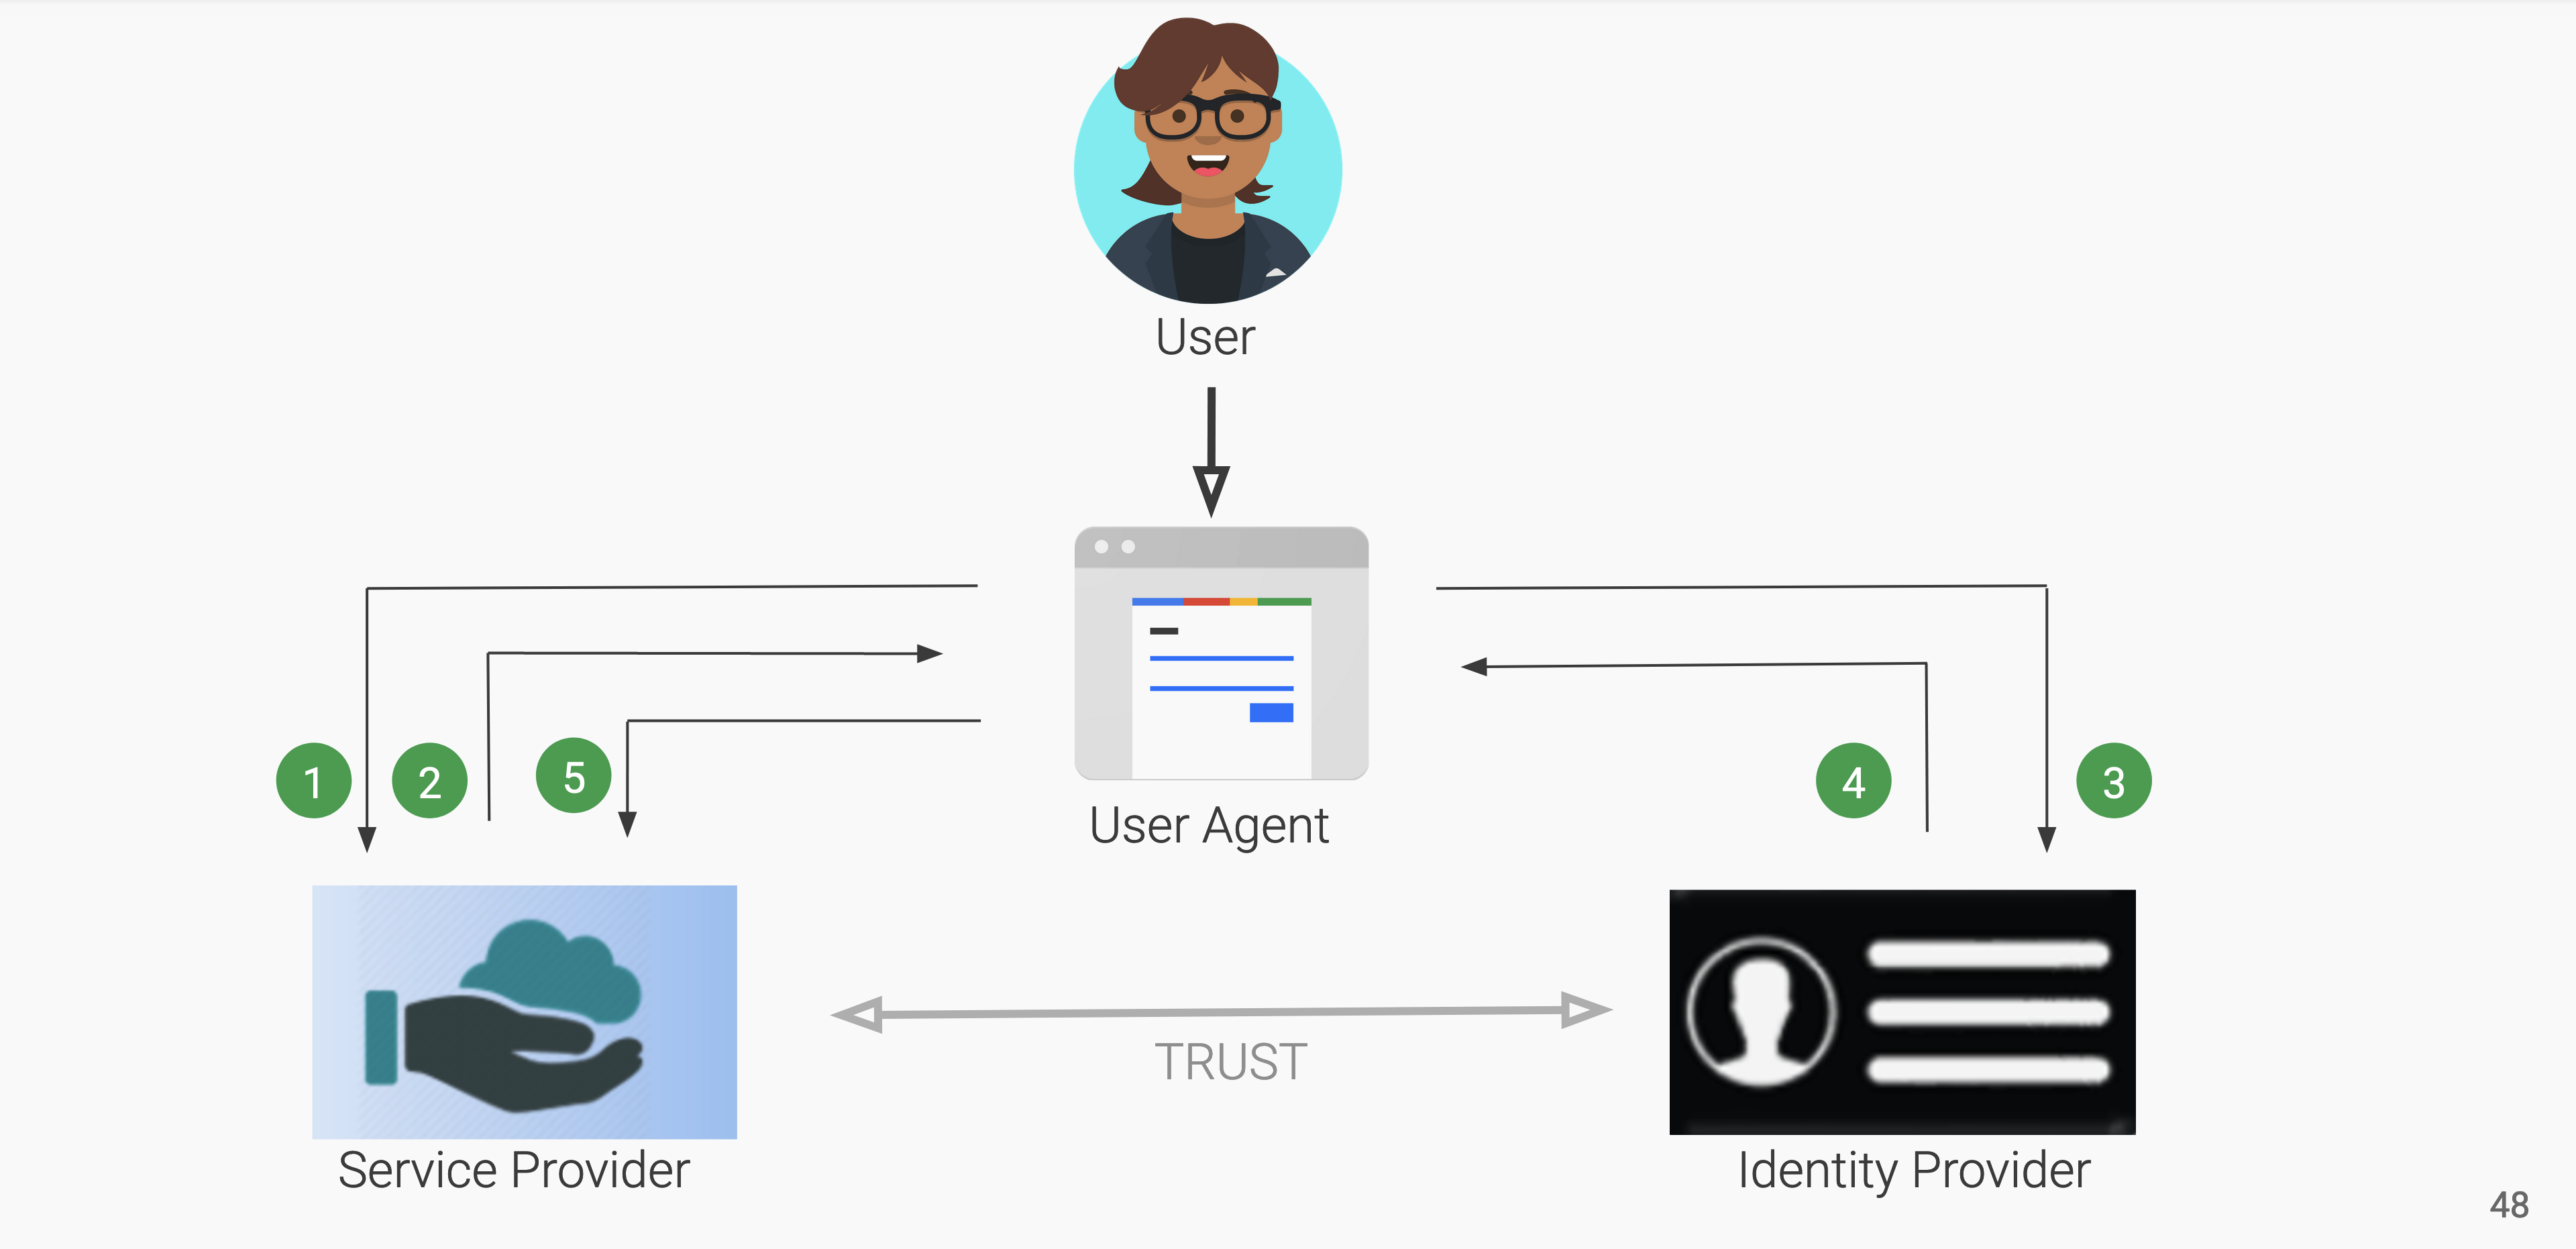
\includegraphics[width=\textwidth]{identity-federation}
\end{frame}

\begin{frame}{Identity Federation}
    %TODO2 fix arrows?
\end{frame}

\section{Exotic Attacks}

\begin{frame}{Exotic Attacks}
    \Large
    \begin{itemize}
        \item OAuth Phishing
        \item Token Theft
    \end{itemize}
\end{frame}

\begin{frame}{OAuth}
    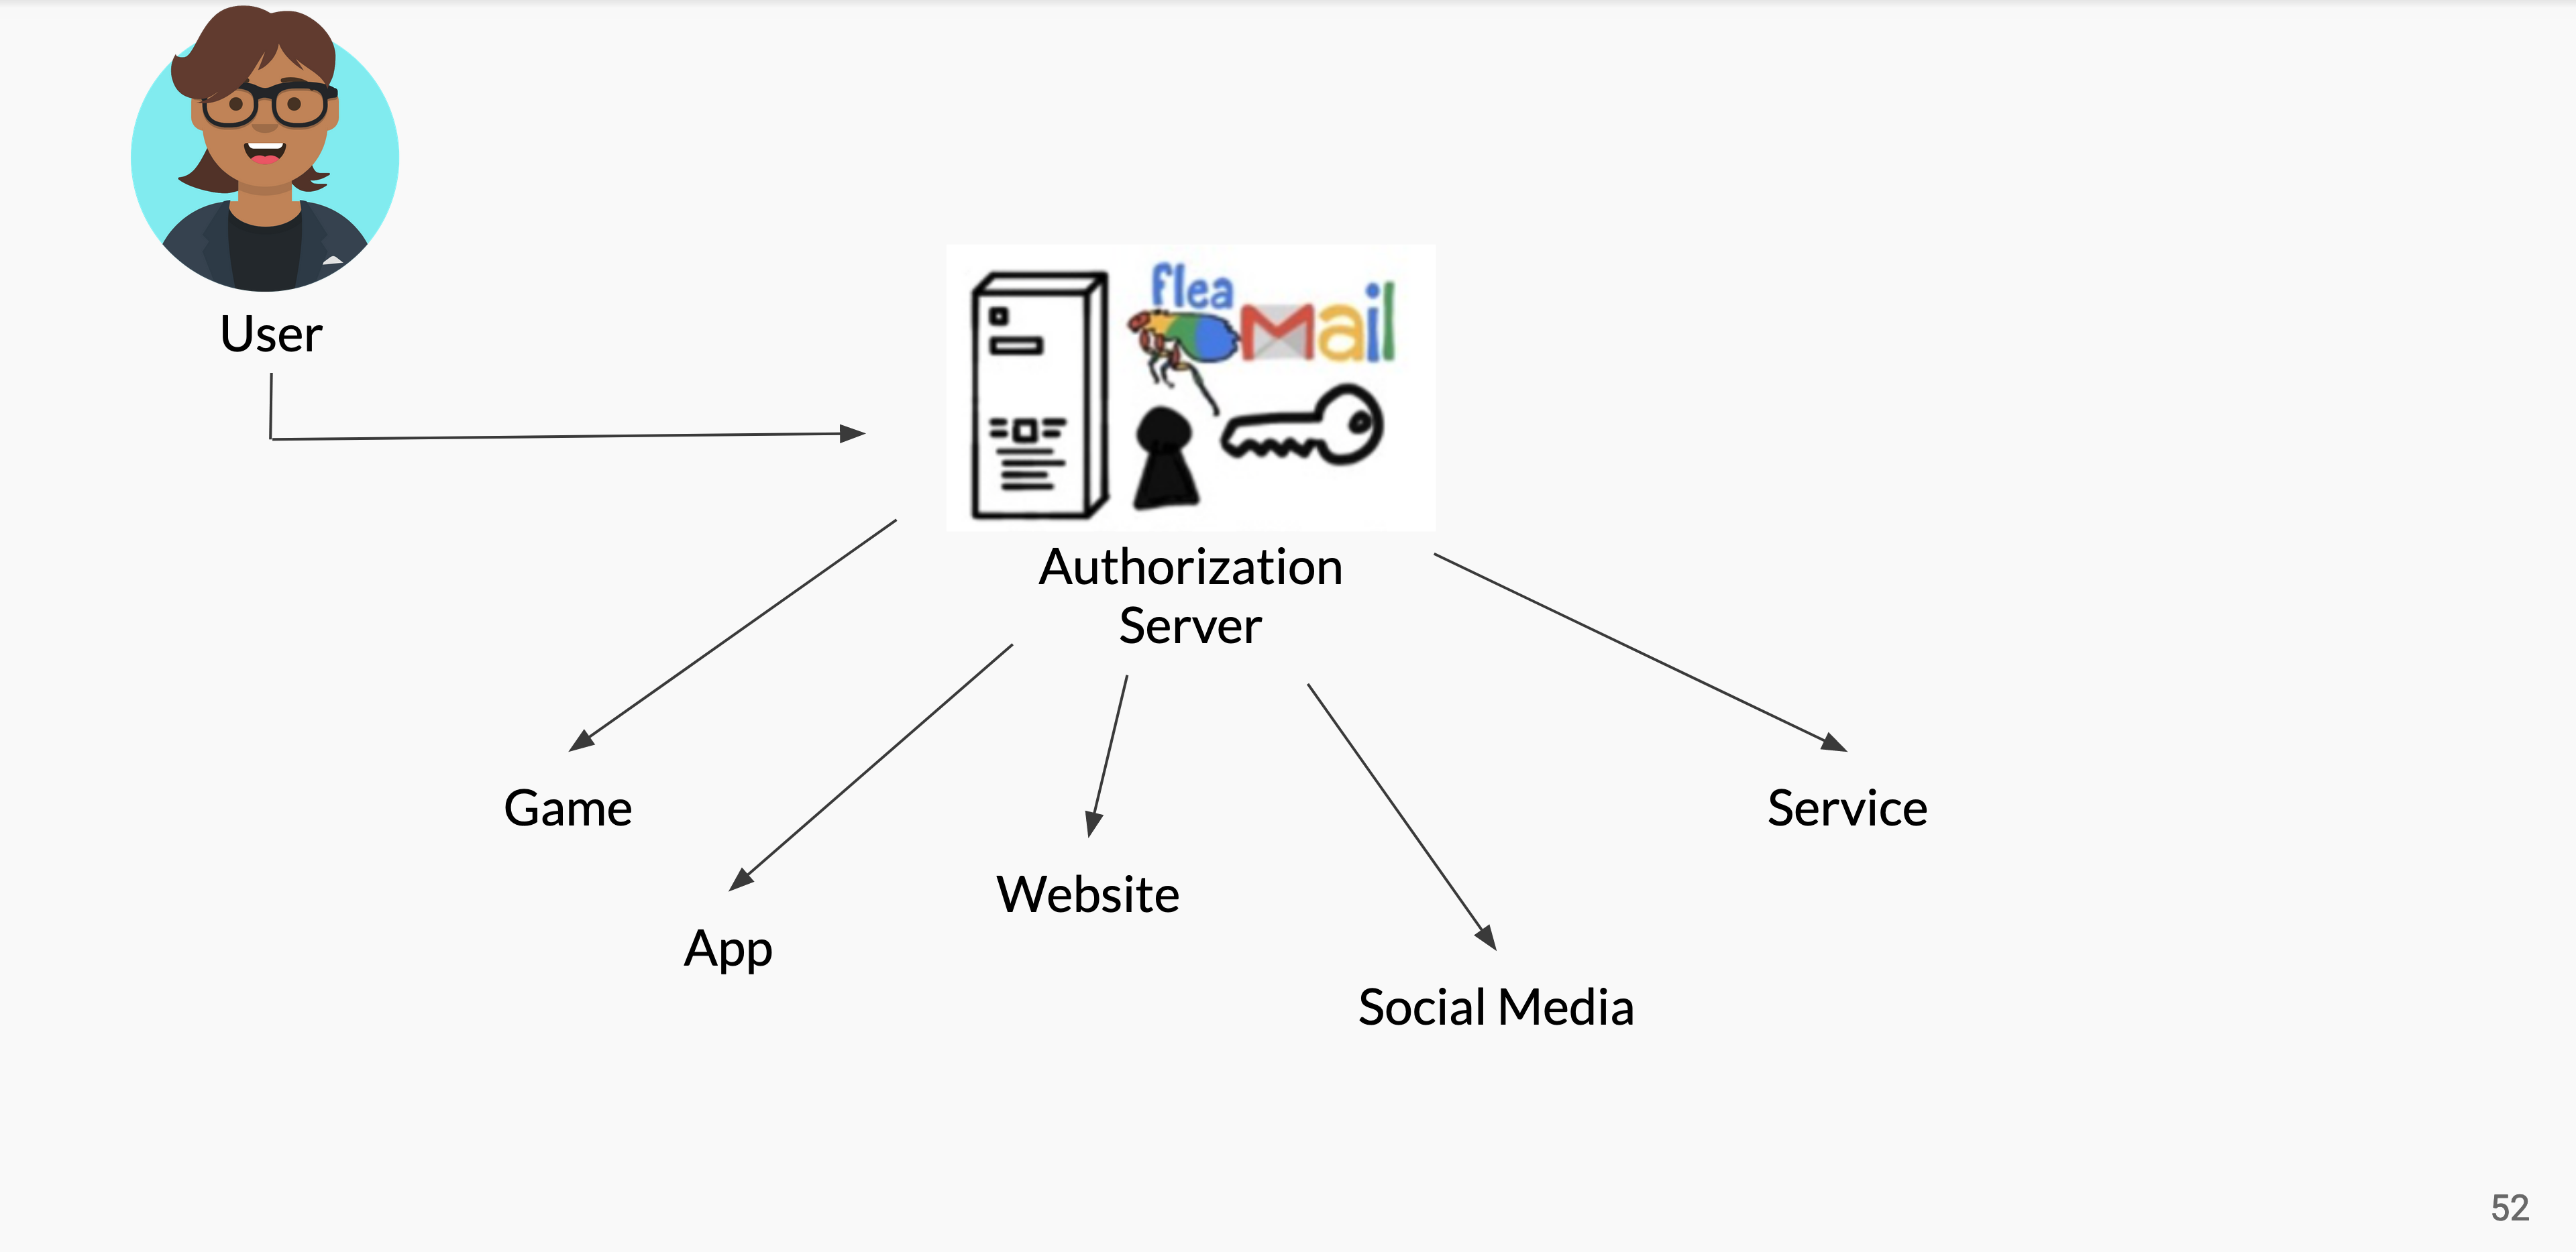
\includegraphics[width=\textwidth]{oauth}
\end{frame}

\begin{frame}{}%TODO3 HOW DO YOU CENTER THIS AAAAAAAA
    \thispagestyle{empty}
    \centering
    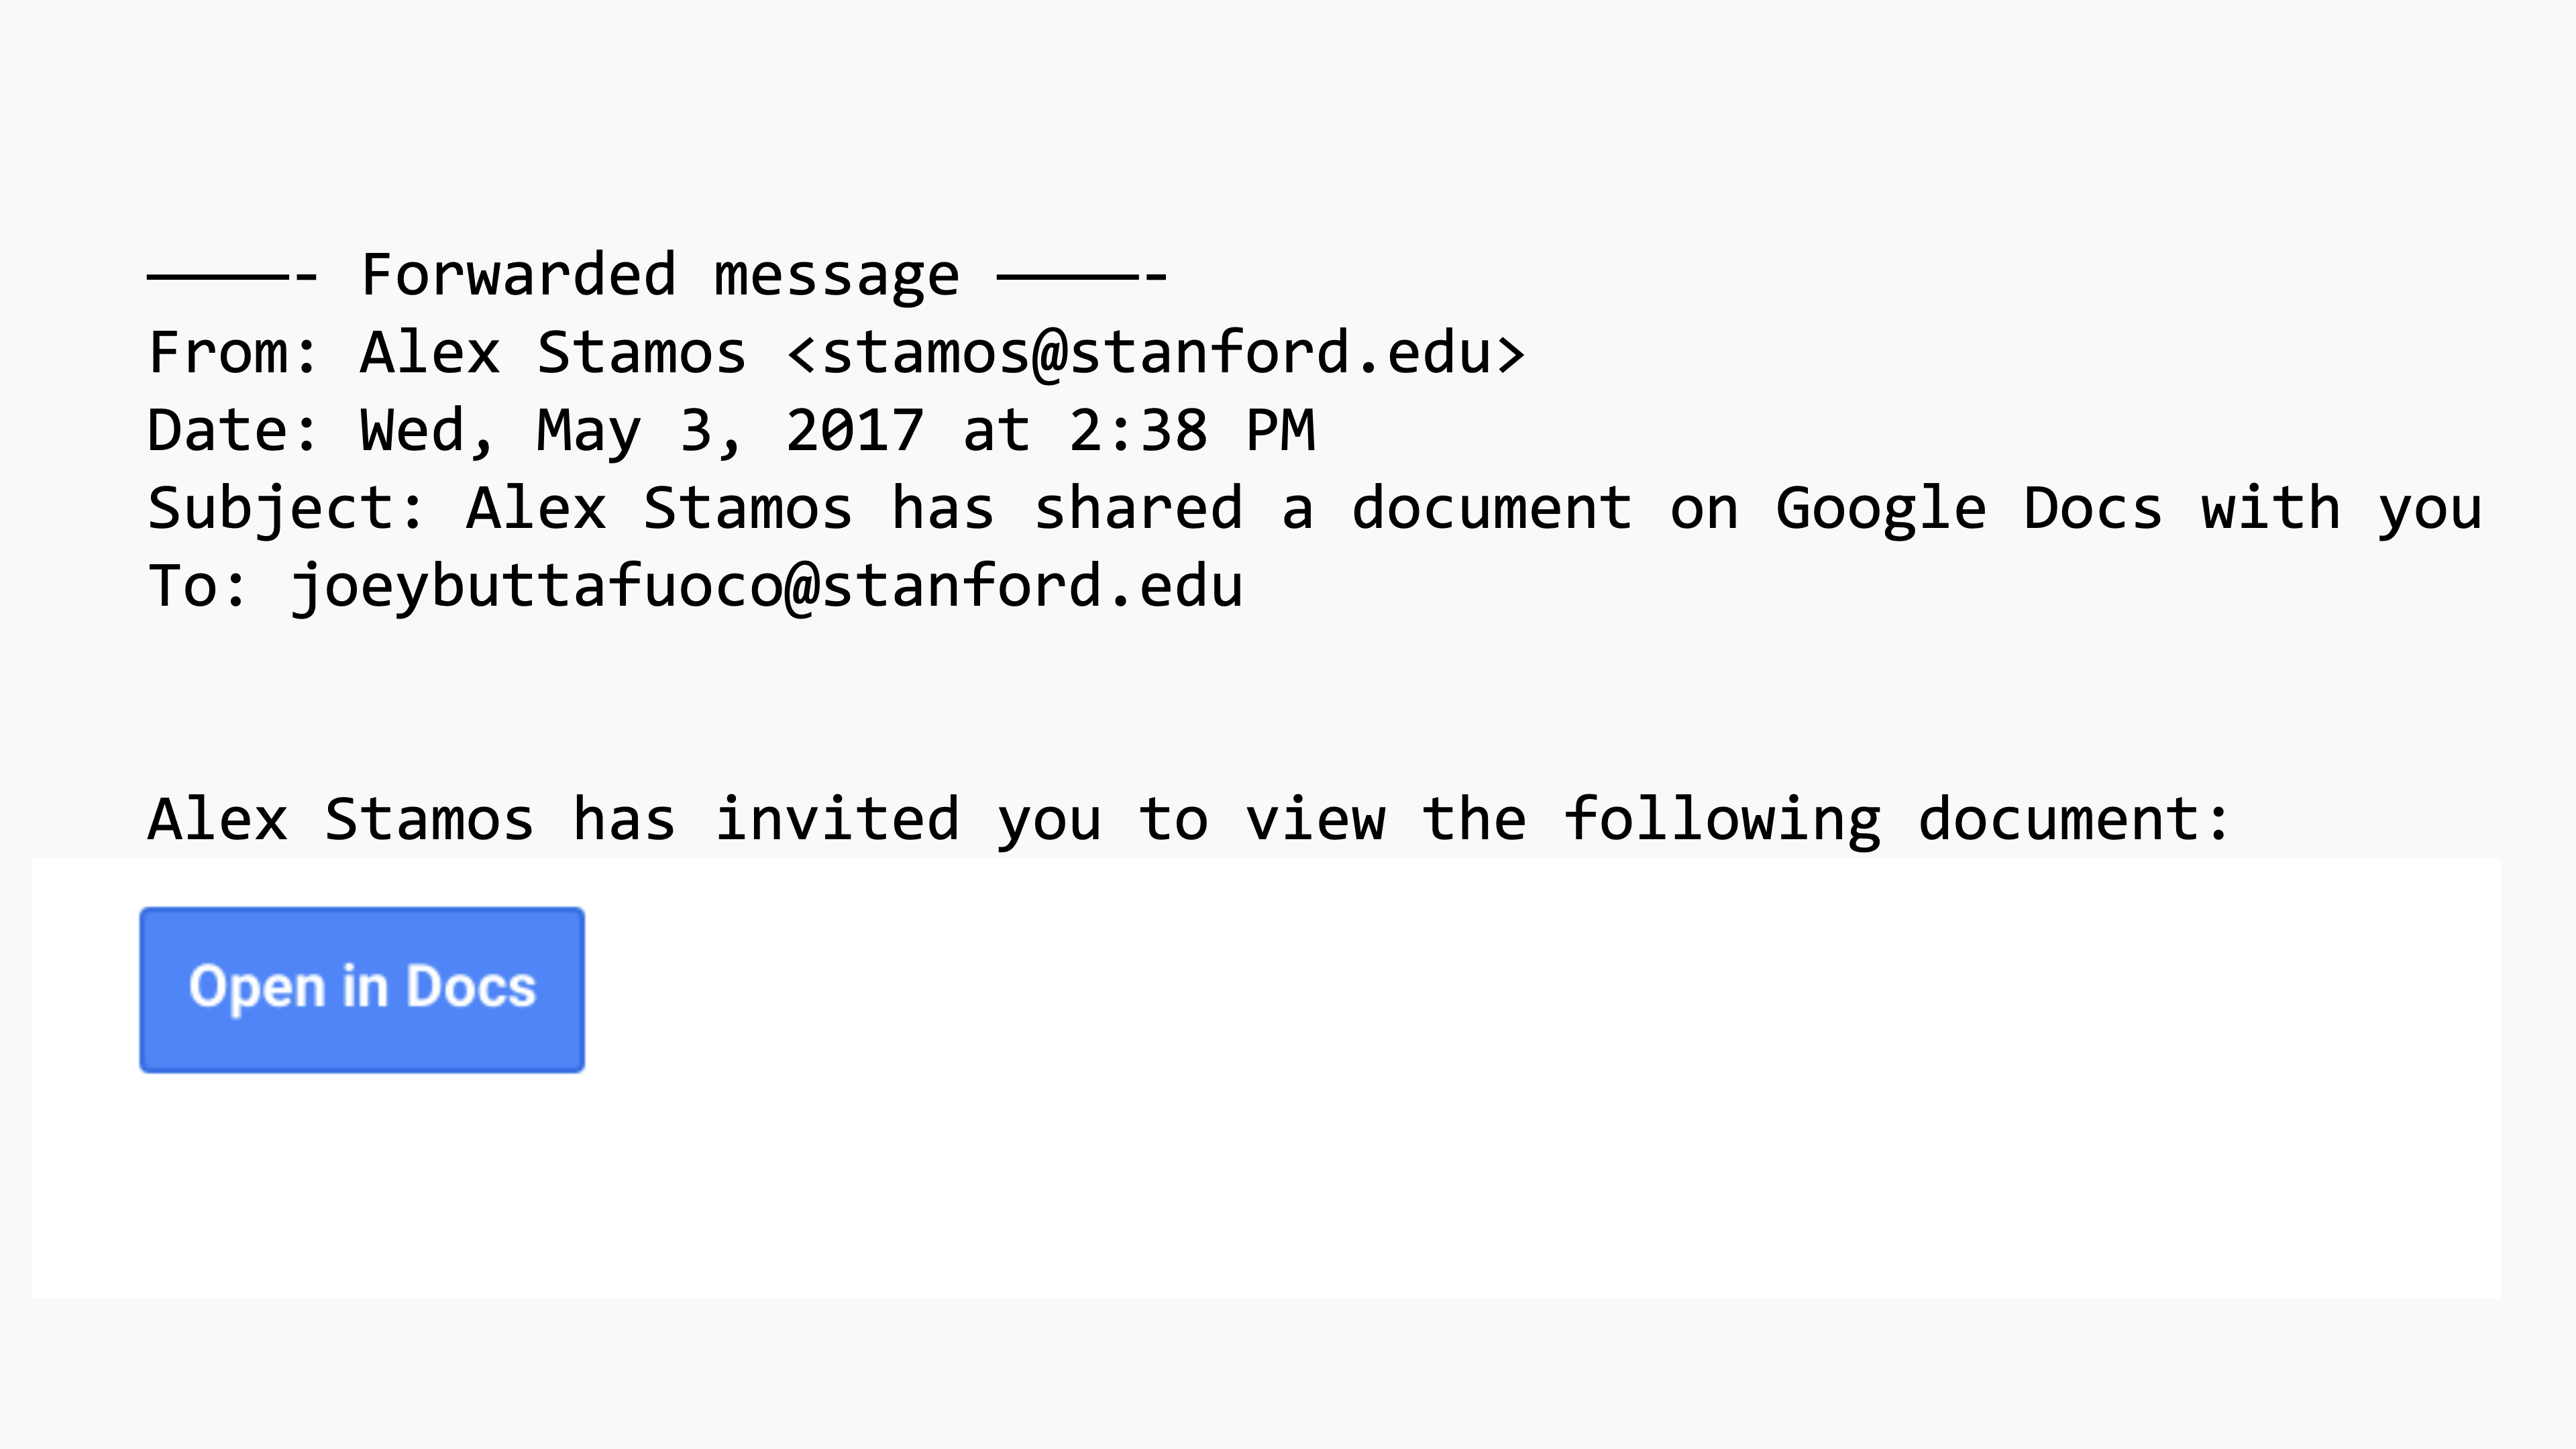
\includegraphics[width=\textwidth]{phishy}
\end{frame}

\begin{frame}{}%TODO3 cursed alignment
    \thispagestyle{empty}
    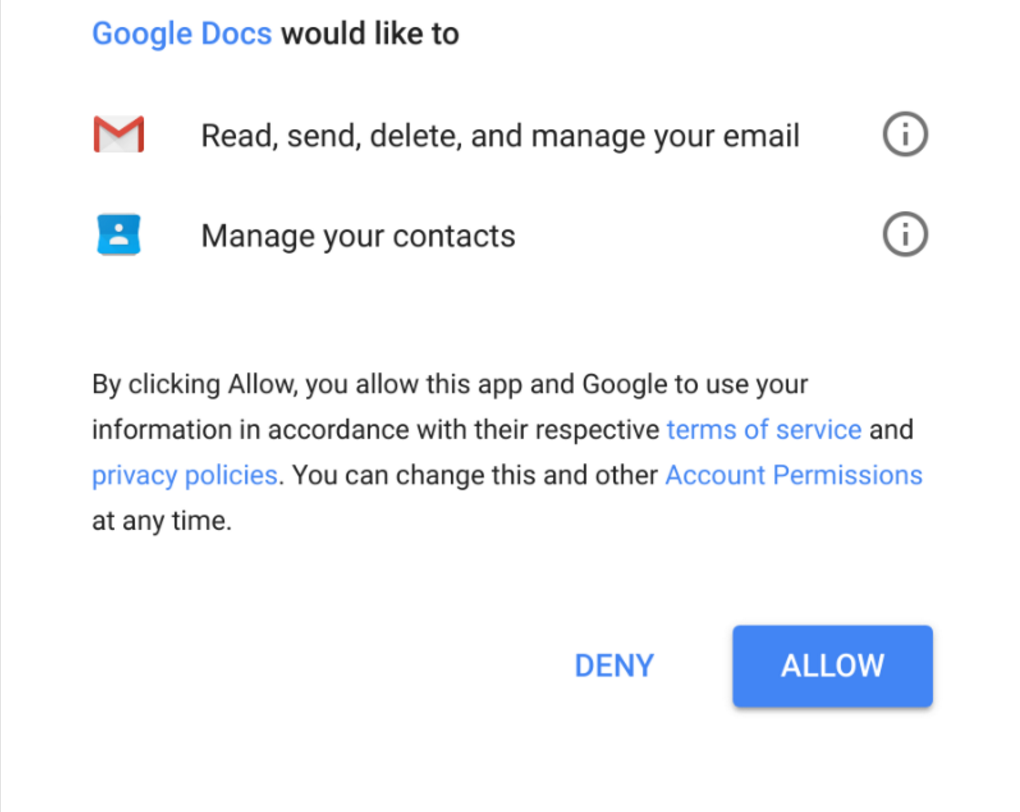
\includegraphics[height=\paperheight]{google-docs-permissions}
\end{frame}

\begin{frame}{Stealing Access Tokens}
    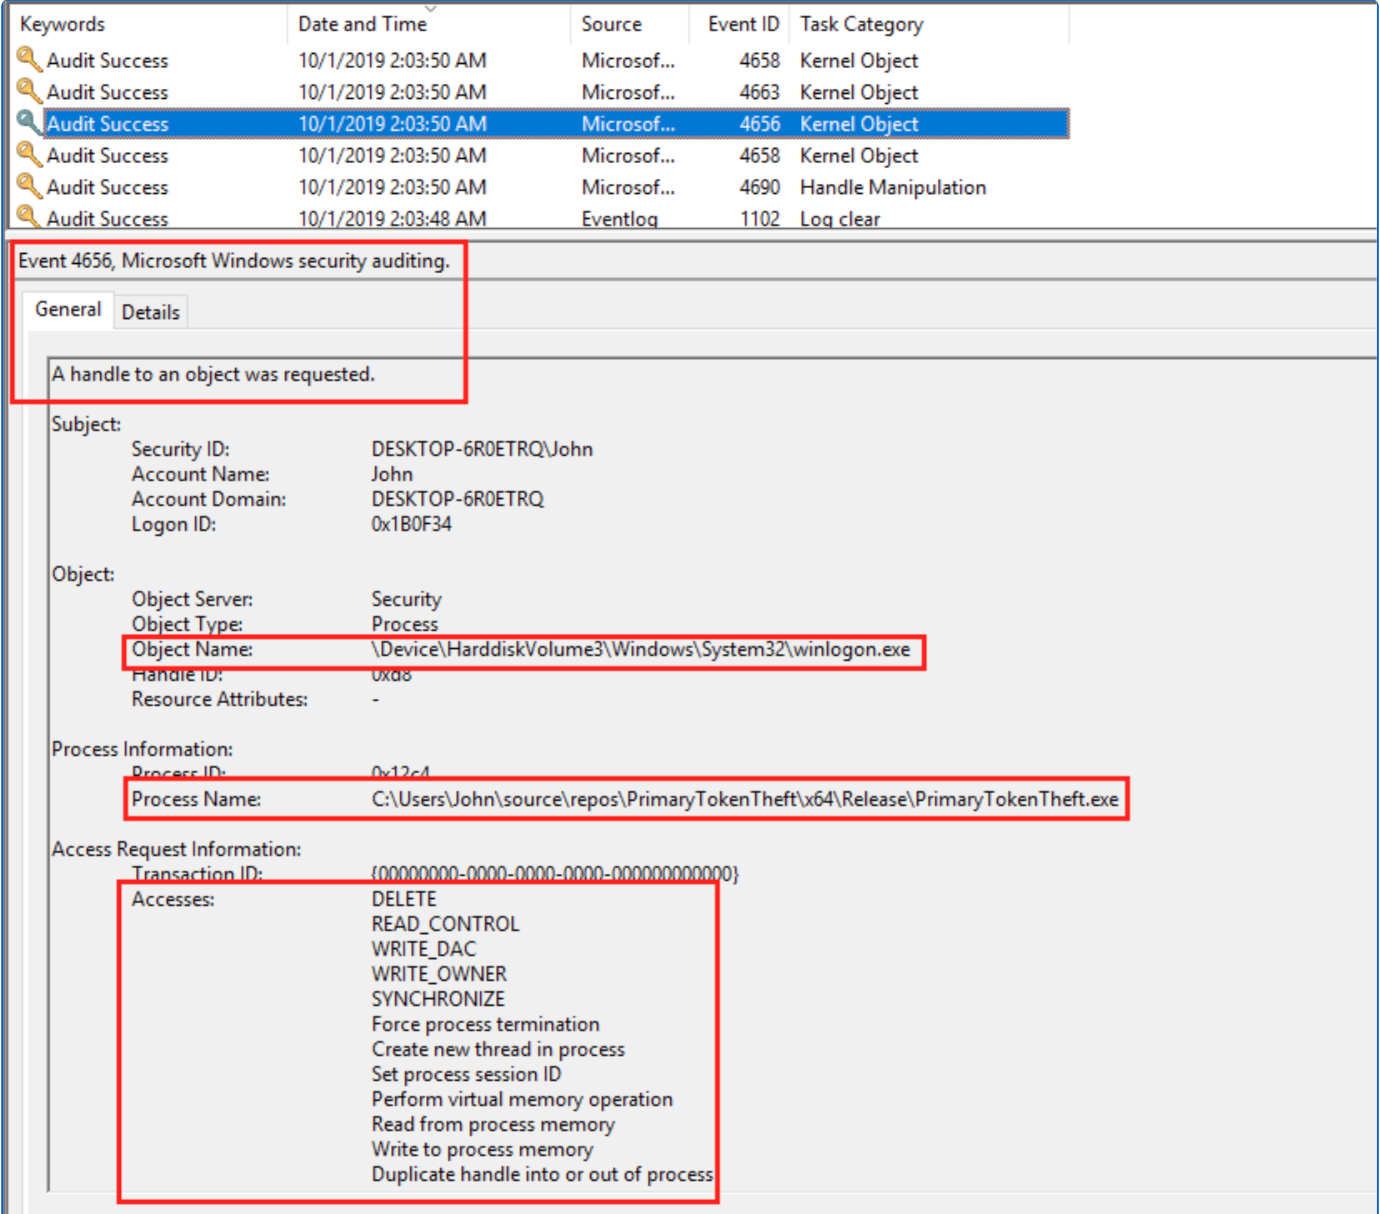
\includegraphics[width=0.95\textwidth]{stealing-access-tokens}
\end{frame}

\begin{frame}{}
    \begin{columns}
        \column{0.6\textwidth}
            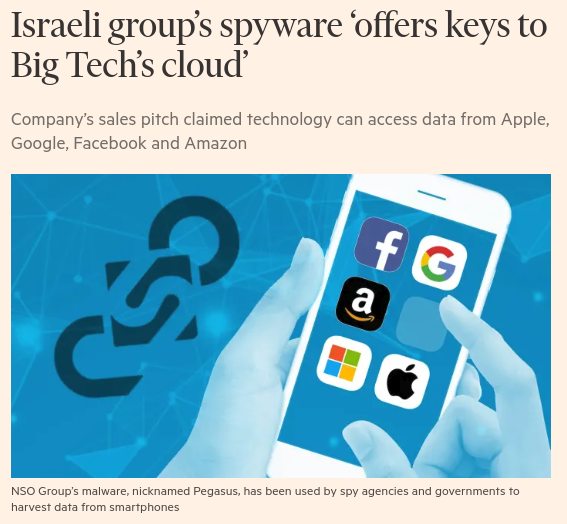
\includegraphics[width=\textwidth]{nso-article}
        \column{0.4\textwidth}
            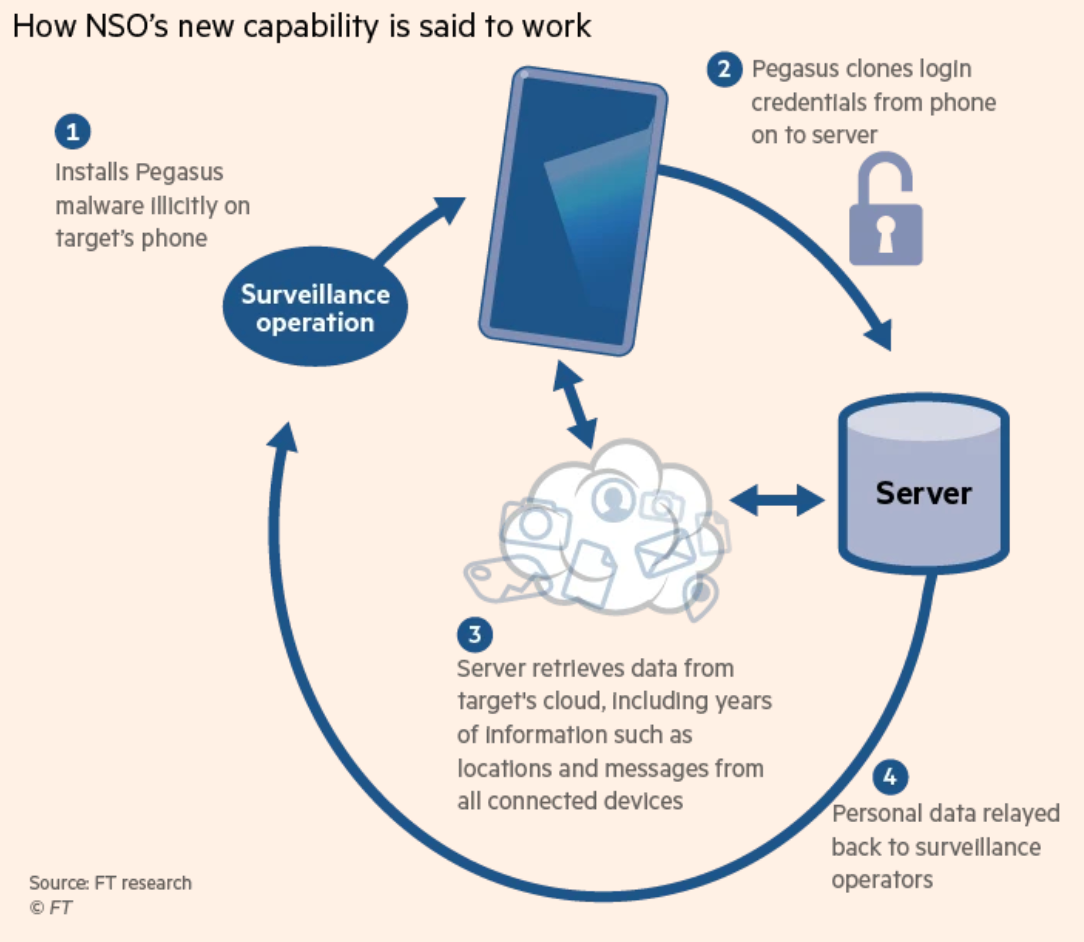
\includegraphics[width=\textwidth]{nso-pegasus-diagram}
    \end{columns}
\end{frame}

\begin{frame}{Risk and Incident Sharing and Coordination}
    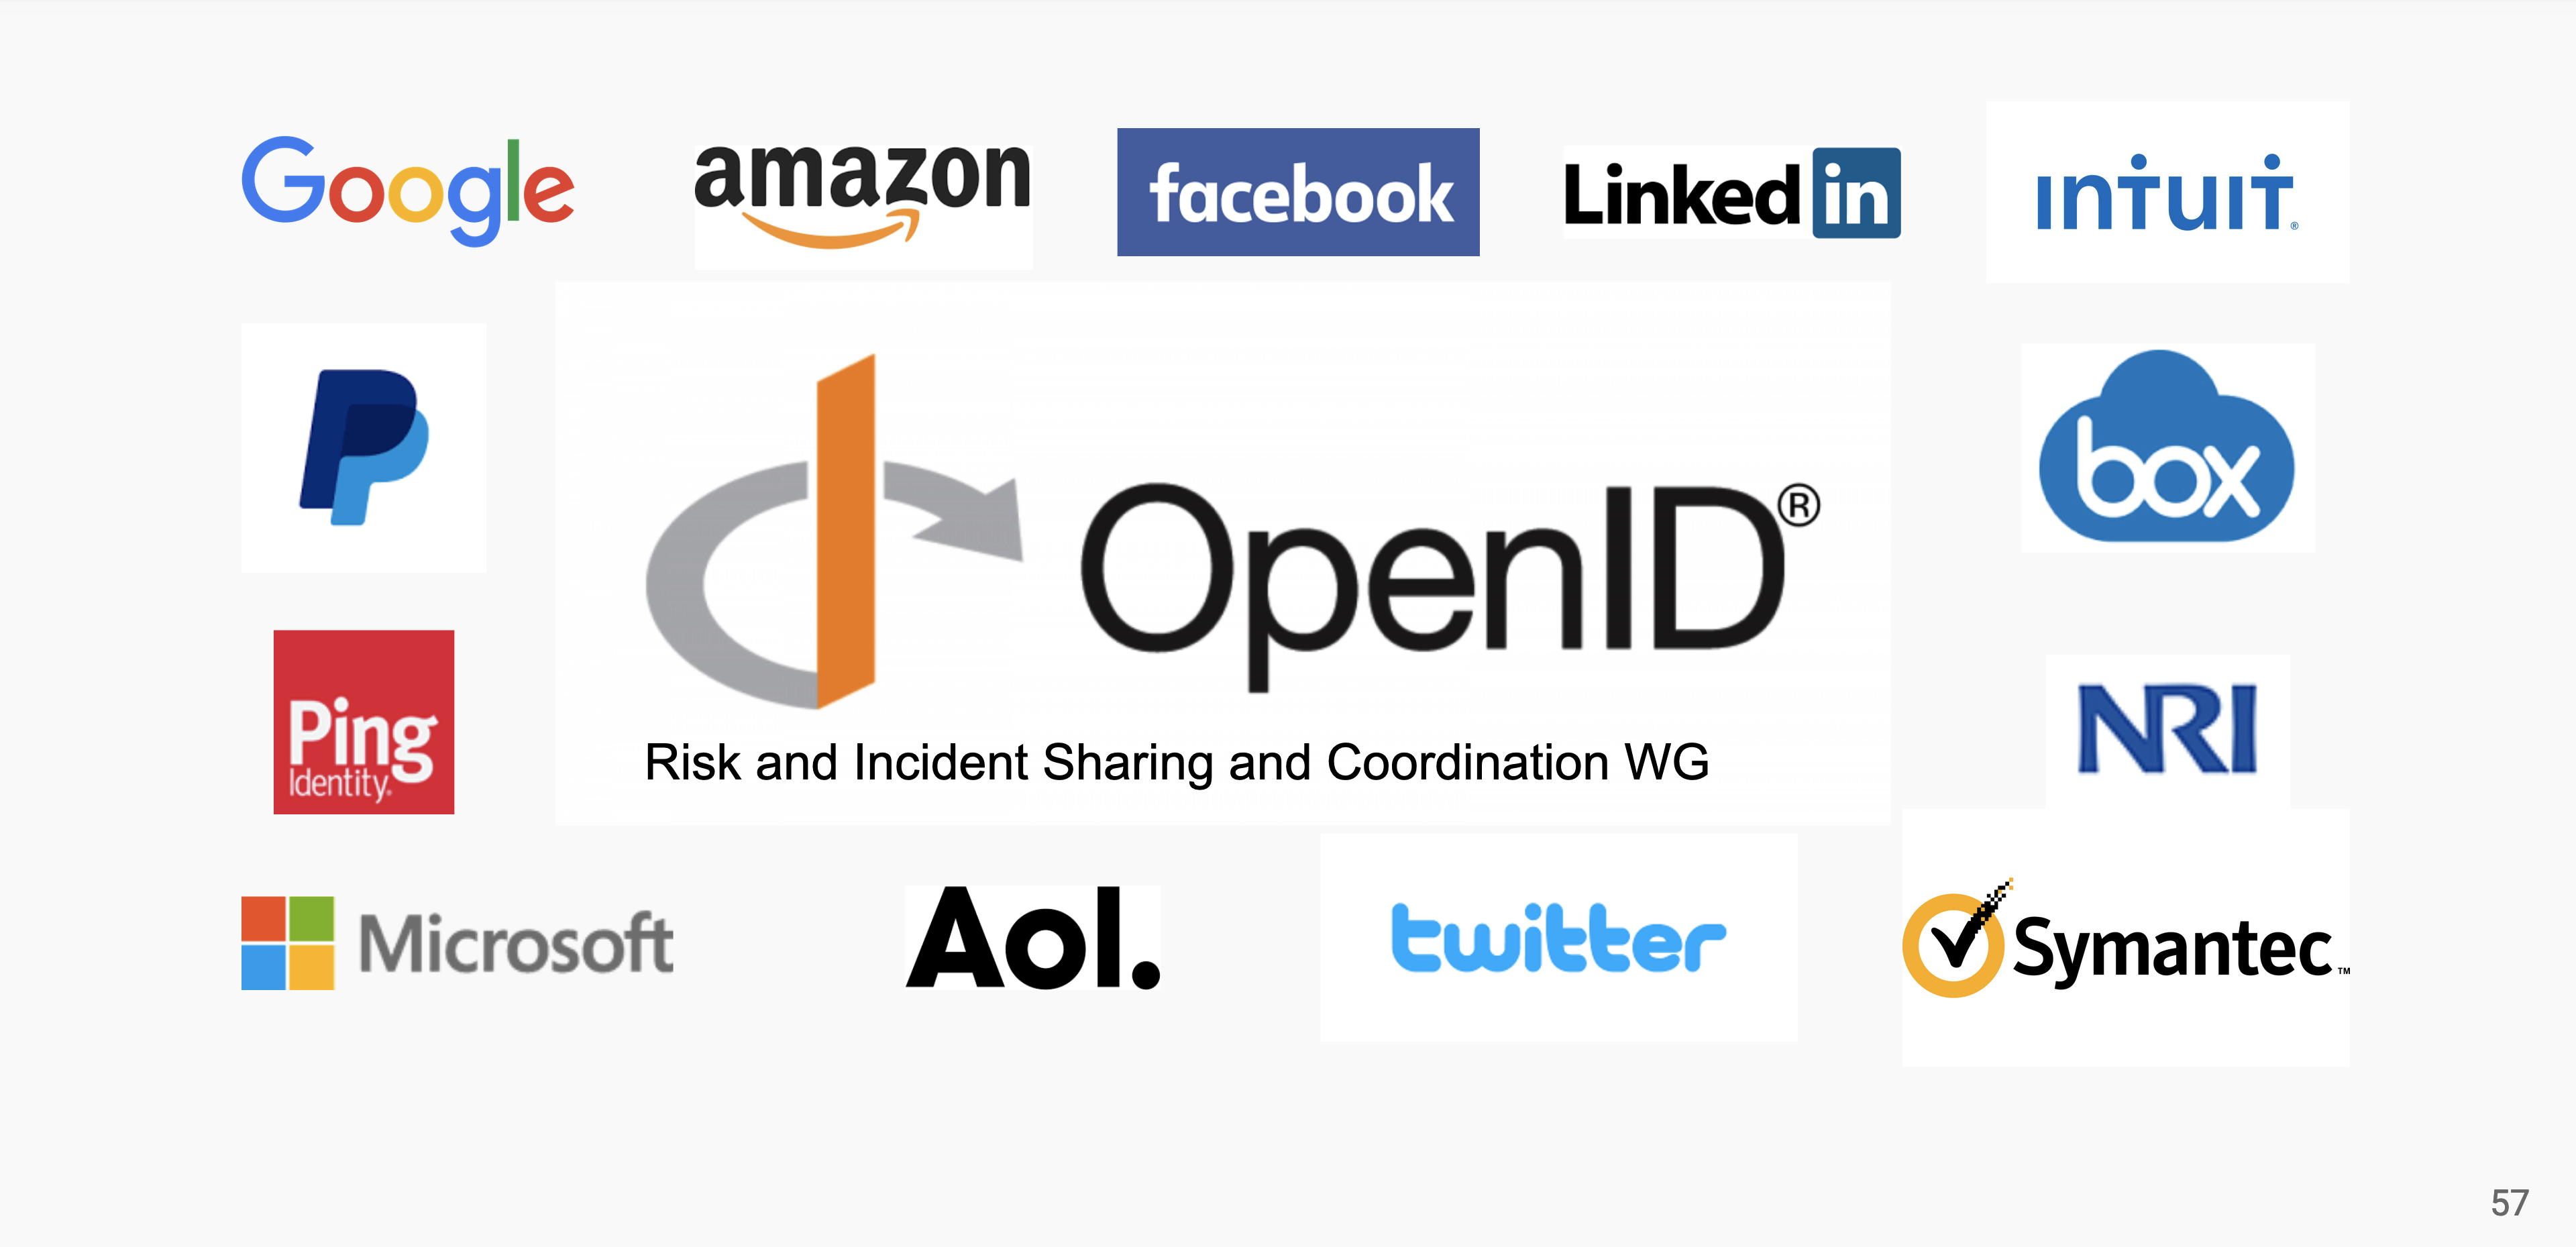
\includegraphics[width=\textwidth]{openid}
\end{frame}

\begin{frame}{Where Is This Going?}
    After taking over an account, what do the attackers do?\\~\\
    Over the next few weeks, we’ll cover the spectrum from simple, commercial monetization, to more nuanced forms of reputation hijacking, to data theft and weaponization
\end{frame}

\backpage

\end{document}